% !TEX TS–program = pdflatexmk

\documentclass[man, floatsintext]{apa6} 
\usepackage[american]{babel}
\usepackage{textcomp}
\usepackage{amsmath}
\usepackage{graphicx}
\usepackage{amssymb}
\usepackage{pifont}
\usepackage{tipa}
\usepackage{color}
\usepackage{bbm}
\usepackage{enumitem}
\usepackage{mathrsfs}  
\usepackage{bbm}
 \usepackage{relsize}
 \usepackage[section]{placeins}




\usepackage[utf8]{inputenc}

\usepackage{csquotes}
\usepackage[style=apa,sortcites=true,sorting=nyt,backend=biber]{biblatex}
\DeclareLanguageMapping{american}{american-apa}
\addbibresource{references.bib}



%tables
\usepackage{tabularx}
\usepackage{array}
\usepackage{booktabs}
\usepackage{multirow}
\newcolumntype{L}[1]{>{\raggedright\let\newline\\\arraybackslash\hspace{0pt}}m{#1}}
\newcolumntype{C}[1]{>{\centering\let\newline\\\arraybackslash\hspace{0pt}}m{#1}}
\newcolumntype{R}[1]{>{\raggedleft\let\newline\\\arraybackslash\hspace{0pt}}m{#1}}
\newcommand{\possessivecite}[1]{\textciteauthor{#1}'s (\textciteyear{#1})}
\renewcommand{\exp}{\text{exp }}
%\renewcommand{\baselinestretch}{1}


\definecolor{PinkyPurple}{RGB}{178,0,178}
\newcommand{\jd}[1]{\textcolor{PinkyPurple}{\textbf{[jd: #1]}}}

\definecolor{CornflowerBlue}{RGB}{100, 149, 237}
\newcommand{\add}[1]{{\color{CornflowerBlue} #1}}


\newcommand{\eref}[1]{(\ref{#1})}
\newcommand{\tableref}[1]{Table~\ref{#1}}
\newcommand{\figref}[1]{Figure~\ref{#1}}
\newcommand{\appref}[1]{Appendix~\ref{#1}}
\newcommand{\sectionref}[1]{Section~\ref{#1}}

\newcommand{\seb}[1]{}
\renewcommand{\seb}[1]{{\bf \color{red} [seb: {#1}]}}


\usepackage{gb4e}
\noautomath

\newcounter{excounter}

%=====================================================================
%========================= preamble material =========================

\title{I know what you're probably going to say:  Listener adaptation to variable use of uncertainty expressions}

\shorttitle{Listener adaptation to uncertainty expressions}

\author{Sebastian Schuster and Judith Degen}
\affiliation{Department of Linguistics, Stanford University}
\keywords{adaptation; language comprehension; experimental pragmatics; Bayesian cognitive modeling; uncertainty expressions}
\authornote{%We are grateful to Eve Clark, Herb Clark, Noah Goodman, Robert Hawkins, Michael Franke, Dan Lassiter, Chris Potts, Michael Henry Tessler, all members of the ALPS lab,
%and audiences at AMLaP 2018, CoMPrag 2018, CaMP 2018, CMCL 2019, Stanford SemFest 2019, and XPRAG 2019 for many discussions that have made this paper better. 
%We further thank our anonymous reviewers and Sarah Brown-Schmidt for invaluable feedback
%leading to many improvements. All remaining errors are our own.
ACKNOWLEDGMENTS REMOVED FOR REVIEWING
\\
Correspondence concerning this article should be addressed to Sebastian Schuster, Department of
Linguistics, Stanford University, 450 Serra Mall, Stanford, CA 94305. E-mail:
sebschu@stanford.edu.\\
Declarations of interest: none \\
All experimental materials, data, analyses, and model implementations are available at \url{http://github.com/sebschu/adaptation}.}
\abstract{Pragmatic theories of utterance interpretation share
the assumption that listeners reason about alternative utterances that a
speaker could have produced, but didn't. For such reasoning to be successful, listeners must have precise expectations about a speaker's production choices. This is at odds with the considerable variability across speakers that 
exists at all levels of linguistic representation. This tension can be reconciled by listeners adapting to the statistics of individual speakers. While linguistic adaptation is increasingly widely attested, semantic/pragmatic adaptation is underexplored. Moreover, what kind
of representations listeners update during semantic/pragmatic adaptation -- estimates of the speaker's lexicon, or estimates of the speaker's utterance preferences -- remains poorly understood.
In this work, we investigate semantic/pragmatic adaptation in the domain of
uncertainty expressions like \textit{might} and \textit{probably}. In a series 
of web-based experiments, we find 1) that listeners vary in their expectations
about a generic speaker's use of uncertainty expressions; 2) that listeners
rapidly update their expectations about the use of uncertainty expressions after
brief exposure to a speaker with a specific usage of uncertainty expressions; 
and 3) that listeners' interpretations of uncertainty expressions
change after being exposed to a specific speaker.  We present
a novel computational model of semantic/pragmatic adaptation based on Bayesian
belief updating and show, through a series of model comparisons, that semantic/pragmatic adaptation is best captured by listeners updating their beliefs both about the
speaker's lexicon and their utterance preferences. This work has implications for both semantic theories of uncertainty expressions and psycholinguistic theories of adaptation: 
it highlights the need for dynamic semantic representations and suggests that listeners integrate their general linguistic knowledge with speaker-specific experiences to arrive at more precise interpretations.}


%=====================================================================

\begin{document}

\maketitle

\setcounter{secnumdepth}{3}

% Section 1: Introduction

\section{Introduction}


One of the key assumptions about pragmatic reasoning is that listeners reason about alternative utterances when interpreting a speaker's utterance \parencite{Grice1975, Horn1984}. For example, consider the following sentences that give rise to scalar implicatures.

\begin{exe}
  \ex 
  \begin{xlist}
    \ex Alex: Bill ate some of the cookies.
    \ex \label{ex:cookie-inf} $\rightsquigarrow$ Bill did not eat all of the cookies.
  \end{xlist}
  \ex 
  \begin{xlist} 
    \ex Tom: The movie was okay.
    \ex \label{ex:movie-inf} $\rightsquigarrow$  The movie was not great.
  \end{xlist}
  \ex 
  \begin{xlist} 
    \ex Sue: It might snow tomorrow.
    \ex \label{ex:snow-inf} $\rightsquigarrow$  It is not certain that it will snow tomorrow.
  \end{xlist}
\end{exe}
According to Gricean pragmatic theories, listeners assume that a speaker is cooperative and arrive at the inference in (\ref{ex:cookie-inf}) through a counterfactual reasoning process: they reason that if Alex had wanted to communicate that Bill ate all of the cookies, Alex would have uttered the more informative statement \textit{Bill ate all of the cookies}. Assuming that Alex knew the truth regarding the more informative sentence, it must be that the more informative statement is not true, which leads the listener to conclude (\ref{ex:cookie-inf}). Analogous reasoning leads to the inferences in (\ref{ex:movie-inf})  and (\ref{ex:snow-inf}).

Accounts of pragmatic reasoning share the implicit assumption that listeners have precise expectations about the speaker's language use -- specifically, which utterance alternatives were available to the speaker that they didn't use -- in different situations. Listeners can only draw correct pragmatic inferences if they know what a speaker would have said to communicate alternative world states. Arguably, this assumption is valid in many contexts -- after all, languages are highly conventional systems \parencite{Lewis1969}. However, language users also exhibit a great deal of variability in their phonetic, lexical, and syntactic choices \parencite[e.g.,][]{Liberman1967,Weiner1983,Harrington2000,Finegan2001,Allen2003}. For instance, while language users generally agree on the ordering of quantifiers such as \textit{some} and \textit{many} and uncertainty expressions such as \textit{might} and \textit{probably} \parencite{Hammerton1976,JaffeKatz1989}, listeners nevertheless have variable expectations of quantifier use \parencite{Yildirim2016} and there exists considerable inter-subject variability in the interpretation of uncertainty expressions \parencite{Wallsten1986}. This raises a puzzle: how can we reconcile the assumption of stable utterance alternatives required for capturing pragmatic inferences with what 
 considerable variability in speakers' actual language use?

Recent work suggests that listeners deal with variability in language use by adapting to it, i.e., by updating their expectations about a speaker's likely productions \parencite[e.g.,][]{Norris2003,Kraljic2005,Kleinschmidt2015,Kamide2012,Fine2016}. In the domain of semantics/pragmatics, this is a process known as \emph{semantic/pragmatic adaptation}. In a series of experiments, \textcite{Yildirim2016} exposed participants to different speakers whose use of the quantifiers \textit{some} and \textit{many} varied in descriptions of quantities of candies of a particular color like \emph{Some of the candies are green}. After exposure to a speaker, they probed participants' expectations about the speakers' likely descriptions of different quantities of green candies and found that participants indeed formed speaker-specific expectations. However, while the results consistently suggest that listeners update \textit{some} type of expectations, the nature of the expectations that listeners update is unknown. 
In particular, it is an open question whether this kind of semantic/pragmatic adaptation is a result of listeners learning speaker-specific utterance \emph{preferences} or whether listeners form speaker-specific \emph{semantic representations}. Answering this question about the nature of adaptation is  the focus of the work reported here.

%Answering this question can provide important insights not only into the processes leading to semantic/pragmatic adaptation but also into properties of the lexicon. For instance, it is possible that listeners only learn different utterance preferences for different speakers but otherwise maintain static semantic representations of uncertainty expressions. On the other hand, listeners might form speaker-specific semantic representations instead of -- or in addition to -- learning speakers' preferences for certain lexical items over others. The latter case would necessitate incorporating \emph{dynamic} semantic representations into our models of language.  Such dynamicity has been found for content words \parencite[e.g.,][]{Clark1983} \jd{be explicit about what you mean -- i'm not sure i know? depending on waht you mean here this paragraph could end in different ways. also, it'll be important to make sure that the assumption of static semantic representations is a different assumption from the one of knowing what the speaker could have said but didn't, which is what the paper starts out with.}. 

%

%TODO?: revisit this again once i've finished the GD about the implications for the lexicon.


As a starting point for this investigation, we consider adaptation in other linguistic domains. Apart from the work on quantifiers, linguistic adaptation has been observed in  phonetics \parencite{Goldinger1998,Norris2003,Kraljic2005,Kraljic2007,Babel2012,Kleinschmidt2015,Clayards2008}, 
syntax \parencite{Kamide2012,Fine2013,Fine2016,Myslin2016,Kroczek2017},\footnote{Note, 
however, that some of these studies failed to replicate and it is still unclear under what 
circumstances syntactic adaptation can be observed \parencite[see][]{Liu2017,HarringtonStack2018}.} intonation and prosody \parencite{Kurumada2012,Roettger2019}, and with phenomena such as referring expressions
\parencite{Clark1986,Brennan1996,Metzing2003,Horton2005,Brennan2009,BrownSchmidt2009,Hawkins2017}, contrastive inferences \parencite{Grodner2011,Pogue2016}, and lexical associations \parencite{DelaneyBusch2019}. 

For most of these phenomena, there is converging evidence regarding the representations that listeners update during adaptation. At the phonetic level, 
listeners update (at least) their expectations about speakers' \textbf{mapping} between acoustic cues and phonemes \parencite[e.g.,][]{Kleinschmidt2015}.
At the syntactic level, listeners update (at least) their expectations about speakers' \textbf{preferences} 
for different syntactic structures. In contrast, at the semantic/pragmatic level the adaptation process and the 
nature of the updated representations is still poorly understood. This is not surprising considering that it is challenging
to directly probe beliefs about semantic representations or beliefs about speaker preferences without 
a model that can quantitatively link behavioral data to these beliefs. 

Recent advances in probabilistic modeling of pragmatic language understanding within the Rational Speech Act (RSA) framework \parencite{Frank2012,Goodman2016,Franke2016} allow us to formally investigate the two likely candidates for representations that are updated during semantic/pragmatic adaptation mentioned above: \emph{utterance preferences} and \emph{semantic representations}. To elaborate,  
listeners might update their beliefs about speakers' preferences
for producing a particular expression (e.g., a preference for \emph{might} over \emph{probably}) -- analogous to syntactic adaptation. Alternatively, listeners might update their beliefs about a speaker's lexicon, i.e. their mapping between 
words and world states (e.g., the range of event probabilities that \emph{probably} is compatible with) -- analogous to phonetic adaptation. Finally, listeners might track both preferences and mappings.

To illustrate how different beliefs about lexica and utterance preferences can lead to different interpretations, consider the interpretation 
of the uncertainty expression \textit{probably} produced by three different hypothetical speakers. For the sake of this example, 
let us assume the only three expressions that a speaker can choose from are \textit{might}, \textit{probably}, and \textit{almost certainly}.
A listener's beliefs about the three speakers' lexica and preferences are schematically illustrated in Figure~\ref{fig:inference-example}.

\begin{figure}
\center
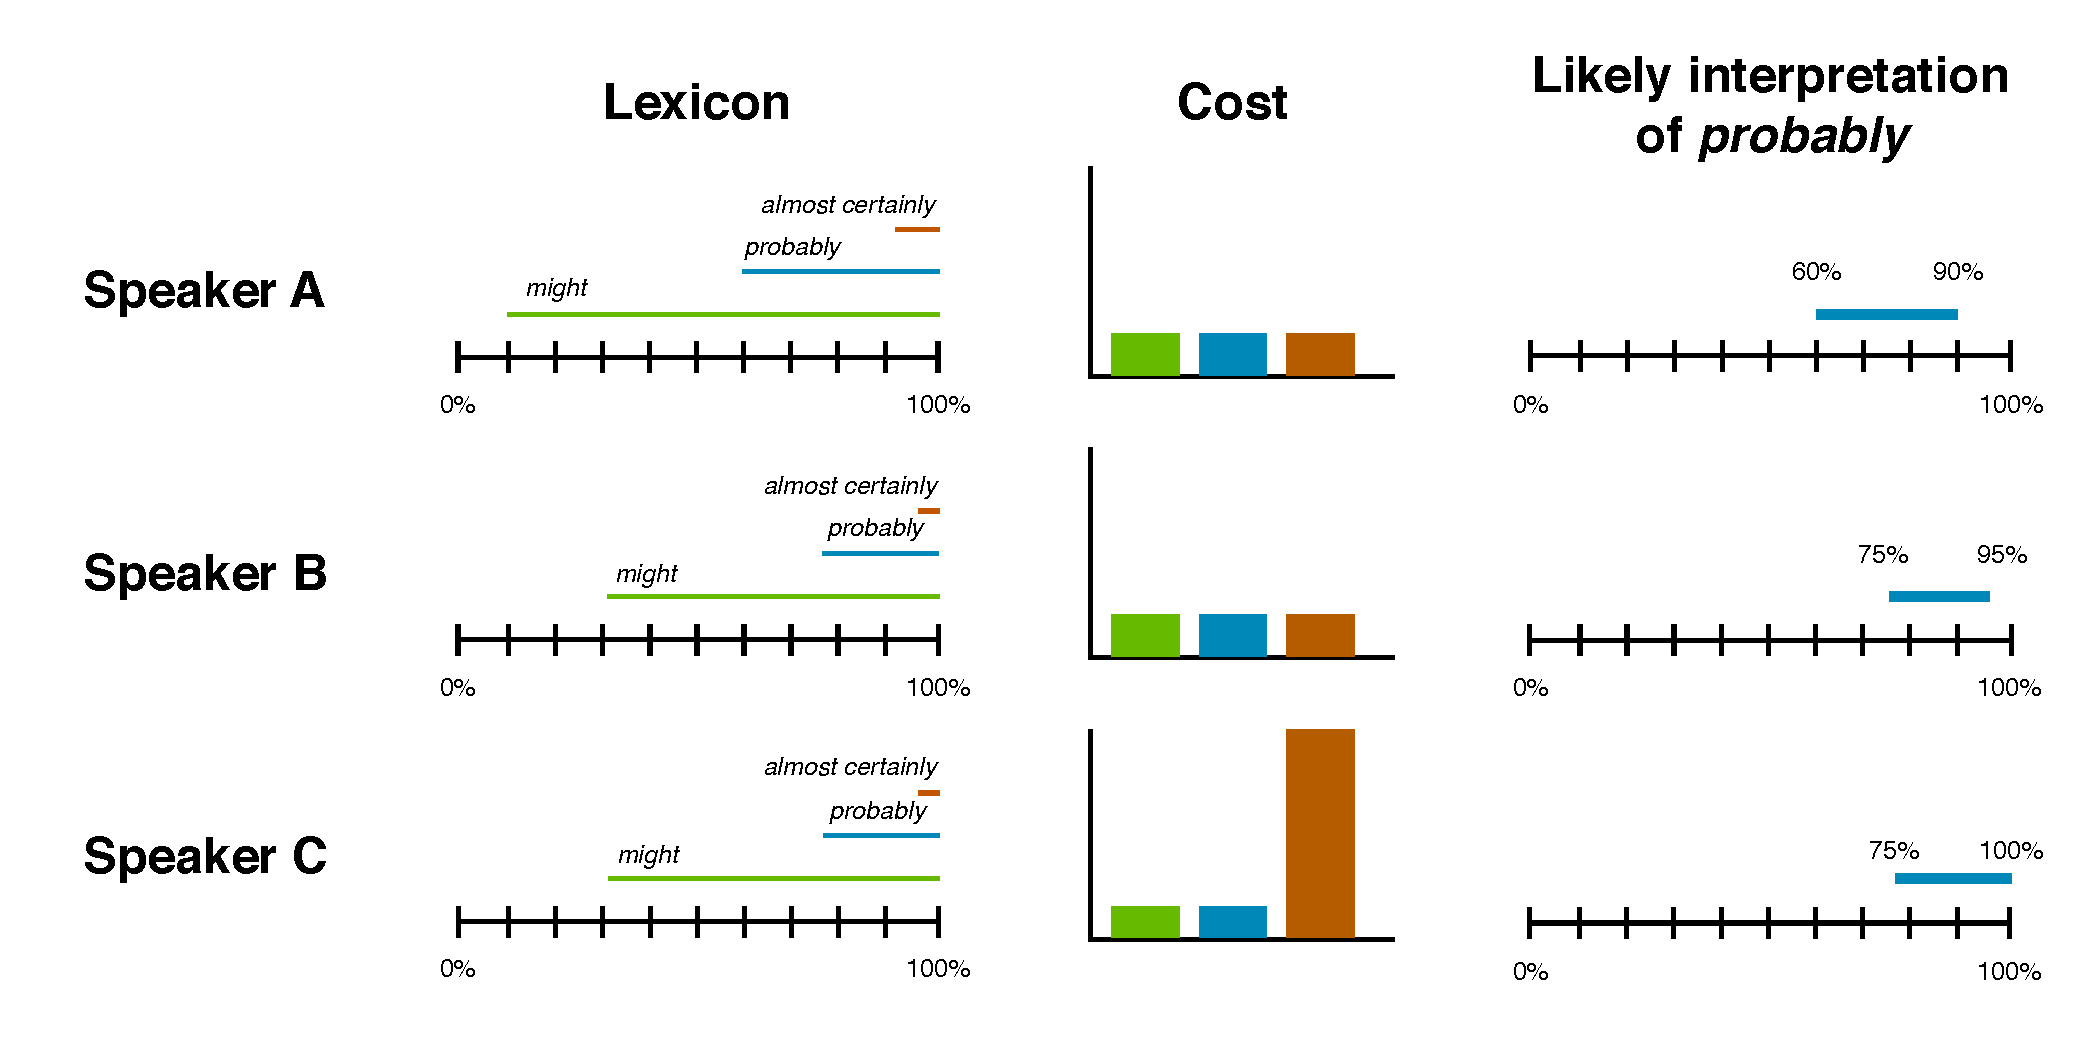
\includegraphics[width=\textwidth]{plots/implicatures.pdf}
\caption{Lexica, utterance preferences and likely interpretation of \textit{probably} for three different hypothetical speakers. The region of the probability scale covered by each line in the Lexicon panel indicates the corresponding expression's literal semantics. Height of bars in the Cost panel indicates the speaker's cost (dispreference) for each expression.}
\label{fig:inference-example}
\end{figure}

First, consider speaker {\bf A}, for whom \textit{might} is true if the described event probability (e.g., of snowing) exceeds 10\%, 
\textit{probably} if the event probability exceeds 60\% and \textit{almost certainly}  if the event probability exceeds 90\%.  If a listener has accurate beliefs about {\bf A}'s mapping between expressions and event probabilities and observes {\bf A}  produce the sentence \emph{It will probably snow}, they will be likely to infer a probability of snowing between 60 and 90\%. As illustrated above, the reasoning follows the schema of a standard scalar implicature \parencite{Grice1975, Horn1984}: if  {\bf A} had intended to communicate a probability above 90\%, they could have said \emph{It will almost certainly snow}, which would have been more informative and equally relevant. Assuming the speaker knows the actual event probability and is cooperative, it is therefore likely that the intended probability is not above 90\%.\footnote{Under a standard Gricean view, the negation of the stronger alternative is inferred categorically. However, we adopt probabilistic language here in keeping with recent results that scalar inferences are more aptly viewed as probabilistic inference under uncertainty \parencite{Goodman2013}.} 

Now, consider speaker {\bf B}, for whom \textit{might} is true if the event probability exceeds 30\%, 
\textit{probably} if the event probability exceeds 75\% and \textit{almost certainly}  if the event probability exceeds 95\%. If a listener has
accurate beliefs about {\bf B}'s mappings, they will be likely to infer, via the same reasoning as above, a chance of snow between 75\% and 95\% when they hear {\bf B} produce the same sentence, \textit{It will probably snow}.

Finally, consider speaker {\bf C}. {\bf C} uses the same mapping between expressions and event probabilities as {\bf B}. However, {\bf C} has a strong preference against 
producing \textit{almost certainly}. If a listener has accurate beliefs about {\bf C}'s lexicon and production preferences, 
they will be likely to infer a chance of snow between 75\% and 100\% when they hear {\bf C} produce \textit{It will probably snow} since they will not
consider  \textit{almost certainly} a likely alternative. That is, the scalar inference will be blocked by the additional knowledge of the speaker's production preferences. 

Thus, a listener who tracks the variability in these hypothetical speakers' lexica and production preferences will draw on average more accurate inferences about the world than one who commits to a particular lexicon without updating it. We investigate the nature of the representations updated during semantic/pragmatic adaptation in the the domain of uncertainty expressions, i.e., words or phrases that can be used to express uncertainty, as used in descriptions of potential future events. These expressions include epistemic modals such as \textit{might}, 
and \textit{could} \parencite[see, for example,][]{Kratzer1991,Hacquard2011}, probability operators such as \textit{probably}, but also phrases such as \textit{it looks like}, which have been primarily investigated in the experimental pragmatics literature (e.g., \cite{Kurumada2014,Pogue2018}).

Uncertainty expressions have several properties that make them a good testing ground for studying semantic and pragmatic
adaptation. First, there is no consistent mapping between uncertainty expressions and event probabilities \parencite[e.g.,][]{Clark1990,Pepper1974}, which suggests that listeners have to rely on additional contextual information (such as speaker identity)
if they want to infer an event probability that a speaker intended to communicate using an uncertainty expression. Second, there is considerable inter-speaker variability 
in the use of these expressions \parencite{Wallsten1986} and therefore it is likely that listeners expect different speakers to use these expressions
differently. Lastly, interpreting uncertainty expressions plays an important role in many everyday situations from the banal -- such as talking about the weather -- to the serious -- such as communicating about health risks \parencite{Berry2004, Lipkus2007, Politi2007} or making financial decisions \parencite{Doupnik2003}. 
Thus, listeners would benefit from tracking  how a given speaker uses these expressions. 

In order to establish the nature of the representations that are updated during adaptation to variable use of uncertainty expressions we proceed through the following steps:
\begin{enumerate}
	\item Quantify the variability in listeners' expectations about a generic speaker's production of uncertainty expressions (Experiment 1, \sectionref{sec:exp-norming}).
	\item Propose a probabilistic computational model of production expectations about uncertainty expressions that functions as proxy for listeners' baseline generative model of a generic speaker. Evaluate the model on the data from Experiment 1 (\sectionref{sec:model-baseline}). The model is formulated within the Rational Speech Act framework, a probabilistic formalization of Gricean pragmatic reasoning   \parencite{Frank2012,Goodman2016,Franke2016}.
	\item Measure whether and to what extent listeners update their expectations when exposed to a speaker who is either more cautious or more confident in their use of uncertainty expressions than expected under the baseline speaker model (Experiment 2, \sectionref{sec:exp-prod-adaptation}).
	\item Extend the baseline model to support adaptation. Create three versions of this model which differ in terms of which model components are updated in response to exposure to simulated cautious and confident speakers: update of only production preferences, only the lexicon, or both. Use model comparison between these three adaptation models as a hypothesis-testing tool to infer which representations undergo adaptation, by evaluating which adaptation model best captures the observed post-exposure expectation data from Experiment 2 (\sectionref{sec:model-adapt}).
	\item To further test the adaptation models, use them to derive predictions about post-exposure interpretation. Measure interpretation and evaluate the model (Experiment 3, \sectionref{sec:exp-model-interpretation}).
\end{enumerate}

We find that listeners indeed update their beliefs about different  speakers' use of uncertainty expressions, and that this adaptation is reflected both in post-exposure measures of production expectations and interpretation. The data are best captured by the adaptation model in which both the lexicon and the speaker's production preferences are updated. We conclude with a discussion of remaining open questions and the implications of our findings for theories
of interactive  \parencite[e.g.,][]{Pickering2004,Pickering2013} and partner-specific language processing \parencite[e.g.,][]{Metzing2003,Horton2005,Horton2016}.

\section{Experiment 1: Pre-exposure ratings}
\label{sec:exp-norming}

We first conducted a norming study, which served the following theoretical and methodological purposes.
First, it served as a methodological check on whether the paradigm is suited for 
manipulating fine-grained event probabilities. 
Second, it addressed the theoretical question of whether listeners vary in their expectations about
a generic speaker's use of uncertainty expressions, by collecting participants' judgments about 
uncertainty expressions they expected speakers to use for varying probabilities of receiving gumballs of a particular color from a gumball machine. 
Third,  the results from this study informed the experimental design of the adaptation experiments 
reported in later sections, by allowing us to both choose which pair of uncertainty expressions to test adaptation on, 
and to determine the particular event probability for which participants had roughly equi-probable expectations 
about which expression of uncertainty a generic speaker would use to report an event with that probability. 
Lastly, we used the data collected in this study to 
estimate population-level prior beliefs for the adaptation model reported in Section 5.

\subsection{Method}

\subsubsection{Participants}
We recruited a total of 420 participants 
(20 per condition) on Amazon Mechanical Turk. 
We required participants to have a US-based IP address and a minimal approval rating of 95\%.
Participants were paid \$1.80 (condition 1), \$1.50 (conditions 2-15),
or \$2.00 (conditions 16-21),
%; condition 6a), 
depending on the number of trials,
which amounted to an hourly wage of approximately \$12--\$15. 

\begin{figure}[th!]
\center
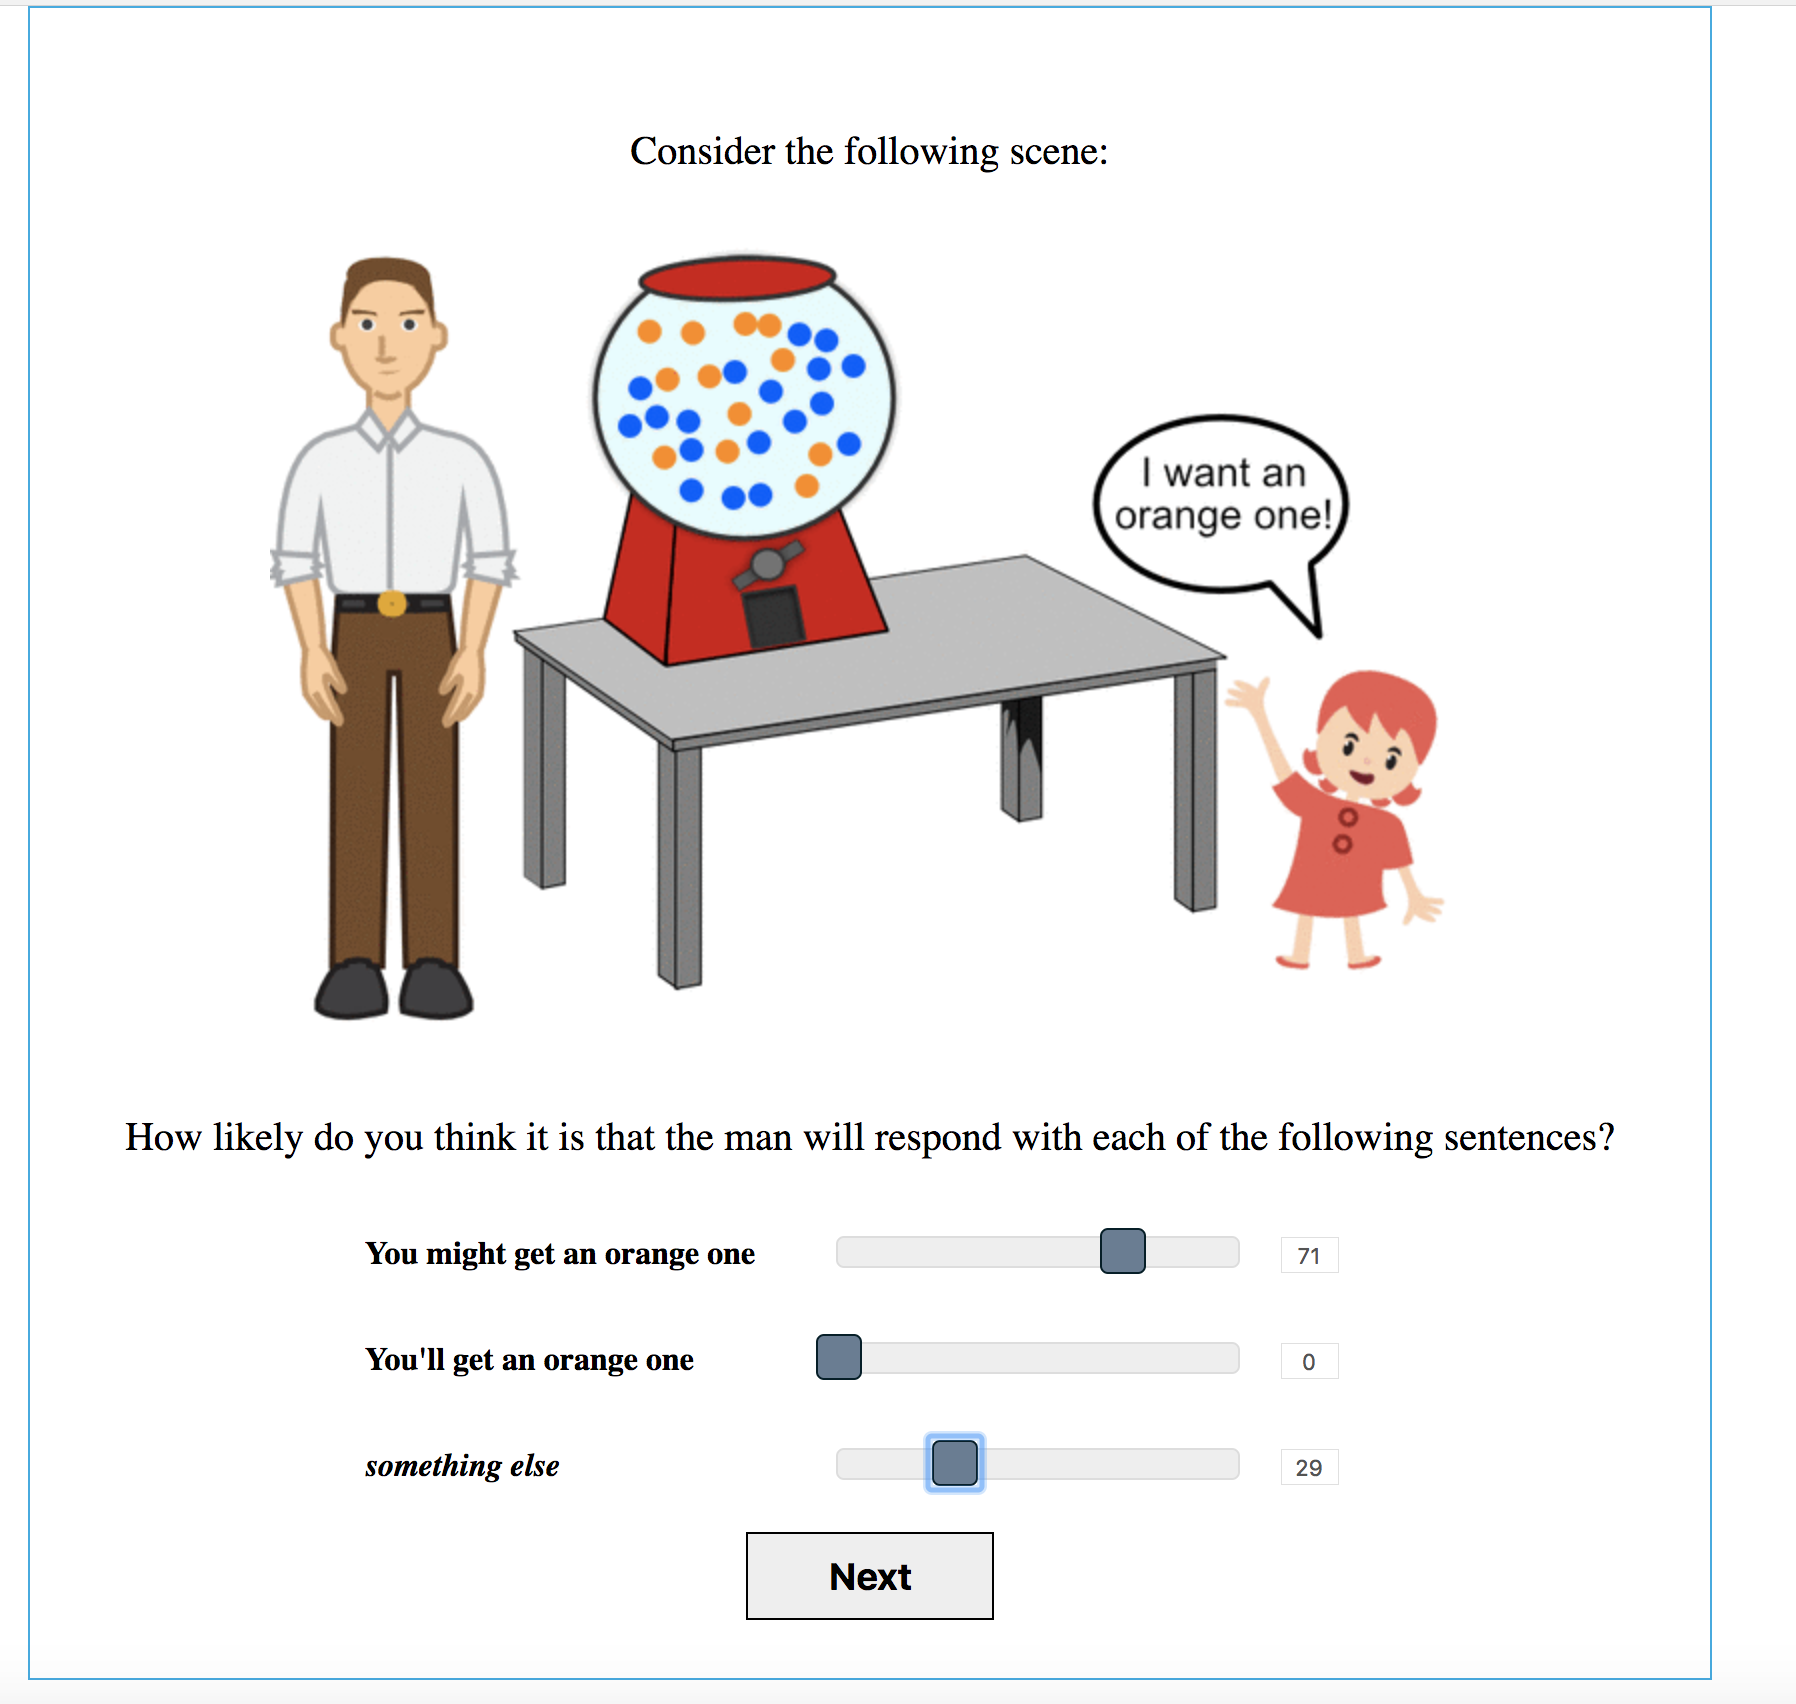
\includegraphics[width=0.7\textwidth, trim={0 0 1.1cm 0},clip]{plots/pre-test-example-trial.png} 
\caption{Example trial in Experiment~1. \label{fig:norming-trial} }
\end{figure}

\subsubsection{Materials and Procedure}
This study was a production expectation experiment intended to probe listeners' expectations about a generic speaker's language use.
Participants were instructed that over the course of the experiment, they would see several scenes with an adult man, 
a young girl, and a gumball machine on a table and 
that the gumball machine is too high up on the table for the girl to see (see Figure~\ref{fig:norming-trial} for an example scene). 
After completing an attention check which asked participants whether 
the girl could see the gumball machine,\footnote{Participants had to go back to the instructions in case they responded incorrectly. This was the case for 41 participants.} 
participants saw a series of scenes  and were asked to rate how likely they thought it was that the 
adult would produce two given responses by distributing 100 points across the two given utterances and the 
blanket \textit{something else} option (\textsc{other}). Sliders automatically jumped back if participants tried to distribute more than 100 points. 
In each scene, the child uttered \textit{``I want a blue one''} (target color: blue) or  \textit{``I want an orange one''} (target color: orange), randomized across participants.\footnote{In condition 1 (\textit{bare-might}), as well as conditions 16-21 (all conditions with \textit{bare not}), the target color was randomized across trials. While randomization of the target color across trials increased the correlation between the ratings for the two colors,  the average ratings for each condition independent of the target color were not affected by this choice. See Appendix A or a detailed discussion of the effect of this manipulation on the ratings.} The gumballs in the machines were tossed around continuously to prevent participants from counting the gumballs
and to make sure that participants did not consider it more likely to get one of the gumballs at the bottom of the machine.
 In each of the 21 conditions, participants saw only  two of the following seven possible adult utterances with different uncertainty expressions:\footnote{In the choice of the investigated expressions, we follow recent work on the interpretation of uncertainty expressions \parencite{Pogue2018} and aim to use naturalistic utterances. We therefore decided against using a frame such as \emph{``It is UNCERTAINTY-ADJ that''} that would have fixed the syntactic structure across items because such a frame would have resulted in less naturalistic expressions like  \emph{``It is possible that''} or  \emph{``It is probable that''}, which are much less common than the expressions we considered (e.g., \textit{might} appears more than 30 times more often than \textit{possible that} in the spoken portion of the Contemporary American English \parencite{Davies2009}). A speaker's use of these rare expressions thus could have triggered additional pragmatic inferences due to violations of the maxim of manner \parencite{Grice1975} that are unrelated to our research questions.}

 \begin{itemize}
\item You'll get a blue/orange one. (\textsc{bare}\footnote{As a notational convention, we refer to utterances with uncertainty expressions in \textsc{small caps} and to the uncertainty expression itself in \textit{italics}. })
\item You might get a blue/orange one. (\textsc{might})
\item You'll probably get a blue/orange one. (\textsc{probably})
\item I think you'll get a blue/orange one. (\textsc{think})
\item It looks like you'll get a blue/orange one. (\textsc{looks like})
\item You could get a blue/orange one. (\textsc{could})
\item You won't get a blue/orange one. (\textsc{bare not})
\end{itemize}


\noindent Within each condition, we manipulated the percentage of target color gumballs across trials, which we take as proxy for the objective probability of receiving a gumball of the target color. 
Each participant saw 3 trials\footnote{In condition 1 (\textit{bare-might}), participants saw each gumball machine 6 times: 3 times when being asked to produce a statement about orange gumballs and 3 times when being asked to produce a statement about blue gumballs. In conditions 15-20 (all conditions with \textit{bare not}), participants saw each machine 4 times: 2 times for each color.} 
for each of the following percentages: 0\%, 10\%, 25\%, 40\%, 50\%, 60\%, 75\%, 90\%, 100\%. We randomized the order of expressions across participants and trials were presented in randomized order.

\subsection{Results and Discussion}

\begin{figure}
\includegraphics[width=\textwidth]{plots/pre\string_test\string_main.pdf} 
\caption{Results from 3 conditions of Experiment~1. Error bars correspond to bootstrapped 95\%-confidence intervals. \label{fig:norming-results-main} }
\end{figure}

Figure~\ref{fig:norming-results-main} shows participants' ratings for different gumball proportions for 3 of the 21 conditions, namely all combinations of the conditions
with the utterances \textsc{bare}, \textsc{probably}, and \textsc{might} (see Appendix~B for the results from the other 18 conditions). 
The results from these three conditions highlight several important properties of participants'
behavior in this experiment that generalize to all conditions.
First, the ratings for individual utterances are influenced by the utterance choices presented to participants.
If we compare the ratings for \textsc{might} in the \textit{bare-might} and the \textit{might-probably} condition, we see that \textsc{might} received high ratings for a larger
range of event probabilities when it is paired with \textsc{bare} than when it is paired with \textsc{probably}. We observe similar effects for the other two utterances.
This suggests that participants are cued towards using the utterances provided in the experiment and that their ratings depend on the presented alternatives -- an effect that
has also been observed for \add{frequency expressions \parencite{Chase1969}} and quantifiers \parencite{Degen2016}.

Second, the results suggest that participants are sensitive to the different event probabilities and that this paradigm is well suited to study 
the mapping between event probabilities and uncertainty expressions. For example, in the \textit{might-probably} condition, participants
provided considerably different ratings when they were presented with a gumball machine with 50\% target color gumballs than when they
were presented with 60\% target color gumballs.

\begin{figure}
\includegraphics[width=\textwidth]{plots/pre\string_test\string_main\string_indiv.pdf}
\caption{Results of three individual participants in the \emph{might-probably} condition of the Experiment~1. \label{fig:norming-results-indiv}}
\end{figure}


Third, in all conditions, the mean ratings are graded and except for the 0\% and 100\% target color gumball trials, the average rating for none of the
utterances is close to 100. There are two potential explanations for this observation. It could be that participants provided categorical ratings, i.e.,
generally assigned 100 points to one of the three options but the category boundaries vary across participants which leads to the graded average ratings.
It could also be that participants' individual ratings are graded which could reflect participants' uncertainty about which utterance a speaker would use 
and that these individual graded ratings drive the  graded average ratings. If we look at individual participants' ratings, it appears to be a combination of both.
Figure~\ref{fig:norming-results-indiv} shows the responses of three individual participants in the \emph{might-probably} condition. These figures show that there 
is a range of gumball proportions for each participant for which they assigned similar ratings to two utterances, which suggests uncertainty about the speaker's 
utterance choice. At the same time, however, this range also differed across participants: Participant \#8, who considered the experimental speaker a 
``\textit{cautious}'' speaker, thought that the speaker would only be likely to use {\sc probably} 
when the objective probability of getting a target color gumball was greater than 0.75, whereas participant \#15, who considered the experimental speaker a ``\textit{confident}'' speaker, thought that  {\sc probably} was a better utterance choice than {\sc might} 
when the objective probability of getting a target color gumball was just greater than 0.5. These observations suggest that for some event probabilities, participants have uncertainty  about a 
speaker's choice of uncertainty expression and that participants have a priori different expectations about how a generic speaker would use these expressions.

This uncertainty and variability seems to be particularly borne out in the \emph{might-probably} condition. For this reason, we chose this pair of expressions
to study listeners' adaptation to variable uses of uncertainty expressions.

\section{Modeling expectations about uncertainty expression productions}
\label{sec:model-baseline}

%Propose a probabilistic computational pragmatics model of the production of uncertainty expressions that functions as proxy for listeners' baseline generative model of a generic speaker. Evaluate the model on the data from Experiment 1. (\sectionref{sec:model-baseline}).

In this section we propose a computational model of expectations about uncertainty expression production that is informed by the data from Experiment 1. This model will serve as proxy for listeners' baseline generative model of a generic speaker and will be used as the basis for investigating adaptation processes in \sectionref{sec:model-adapt}. Experiment~1 confirmed previous findings that participants' expectations 
about how a generic speaker would use uncertainty expressions 
depend on the set of utterances that participants can choose from.
We further found that ratings were graded in part because participants had uncertainty about how a generic speaker would use uncertainty expressions. 
Hence, a model that accounts for participants' beliefs about a speaker's production of uncertainty expressions
 should  (a) be able to capture differences in ratings depending on the availability of alternative utterances;
(b) provide graded predictions about utterance probabilities; 
and (c) be able to capture within-participant uncertainty about probability of use.

Computational game-theoretic models such as the Rational Speech Act 
framework (RSA; \cite{Goodman2016})  are uniquely suited to satisfy the above desiderata.
RSA models are a probabilistic formalization of Gricean pragmatics which model comprehension as Bayesian probabilistic inference. 
They consist of \textit{listener} and \textit{speaker} agents which recursively reason about each other to derive interpretations and choose utterances. 
For our purposes of modeling production expectations, we focus on a model of listener beliefs about a speaker's production model.
  According to  RSA, a {speaker} that wants to
 convey some information to a {listener}
chooses an utterance based on the utterance's utility compared to the utility of alternative utterances. 
The {speaker}'s utterance utility is determined by trading off the informativity of the utterance to a \textit{literal listener} on the one hand and the cost of the utterance on the other.

In defining the informativity of an utterance, we follow previous RSA models of uncertainty expressions (\cite{Herbstritt2019}) 
and assume that uncertainty expressions have a threshold semantics \parencite{Swanson2006,Yalcin2010,Lassiter2016}. That is, for each uncertainty expression $e$ there exists some threshold $\theta_e \in [0,1]$ 
such that an utterance $u_e$ with $e$ is true if the probability $\phi$ 
of the proposition embedded under $e$ exceeds $\theta_e$. 
For example, if we assume the threshold for \textit{might}, $\theta_{might}$, is 0.1, then the statement 
``It might rain this afternoon'' is semantically available to a {speaker} who believes that the probability of rain in the afternoon exceeds $0.1$.
Formally, we base the computation of informativity on a probability distribution from utterances to event probabilities $\phi$, 
which is usually referred to as the \textit{literal listener} $L_0$ in the RSA framework. 

$$L_0\left(\phi \mid u_e, \theta_e\right) \propto P(\phi) \times 
\begin{cases}
1 & \mbox{if } \phi > \theta_e\\
0 & \mbox{otherwise} 
\end{cases} \qquad \mbox{(for positive embedded propositions)}$$
$$L_0\left(\phi \mid u_e, \theta_e^{'}\right) \propto P(\phi) \times 
\begin{cases}
1 & \mbox{if } \phi < \theta_e^{'} \\
0 & \mbox{otherwise} 
\end{cases} \qquad \mbox{(for negated embedded propositions)}$$

According to this formalization, the {literal listener}  randomly draws an event probability $\phi$ from all values above  the threshold $\theta_e$ associated with the uncertainty expression $e$ (or, in the case of negated propositions, from all values below the threshold $\theta_e^{'}$). $P(\phi)$ is a prior distribution over event probabilities, which is independent of the observed utterance.

A \textit{pragmatic speaker} $S_1$ that intends to communicate an event probability $\phi$ then chooses an utterance $u_e$ with uncertainty expression $e$ from a set of utterances $U$ according to a soft-max choice rule \parencite{Luce1959,Sutton1998} such that $u$ is chosen with a probability proportional to the utility for the speaker:
$$S_1\left(u_e \mid \phi, \theta, c\right) \propto exp \left( \lambda \left( \log L_0\left(\phi \mid u_e, \theta_e\right)  - c(u_e)\right)\right)$$
$\lambda$ is a rationality parameter which governs how likely the {speaker} is to choose the utterance that maximizes utility. As $\lambda$ approaches infinity, the {speaker} is more likely to always choose the optimal utterance. As it approaches 0, the {speaker} produces true utterances at random.\footnote{
The absolute value of this parameter is influenced by the literal listener distributions and the cost function. It is therefore complex to determine a reasonable range for $\lambda$ a priori, except that the value should be greater than 0 for the agent to not behave irrationally.} %However, \textcite{Herbstritt2019} inferred $\lambda$ from data for a similar model and found it to be likely in the interval $[4.5;5;2]$, which suggests that we should also expect a similarly large value for $\lambda$ in our setup.} 


\begin{figure}[th!]
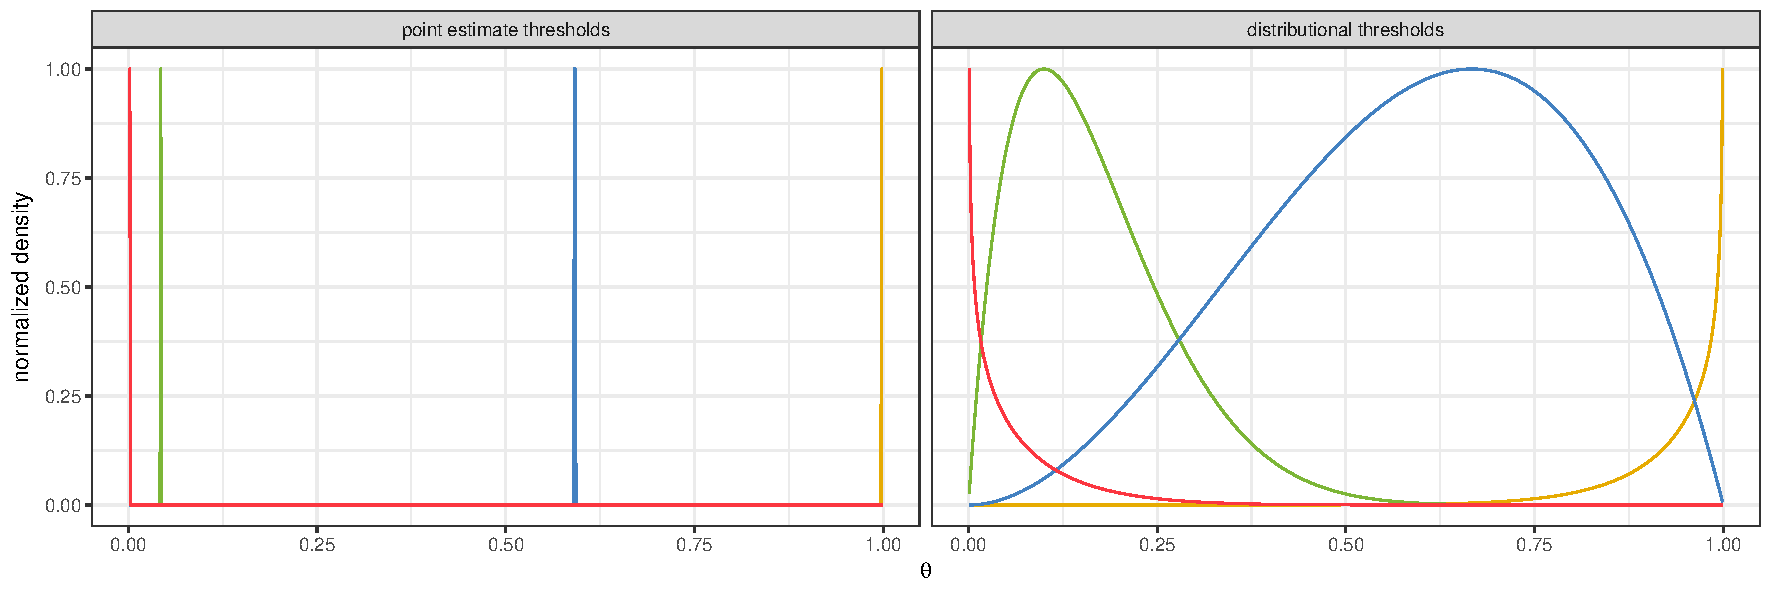
\includegraphics[width=\textwidth]{plots/model-visualization-distributions.pdf}

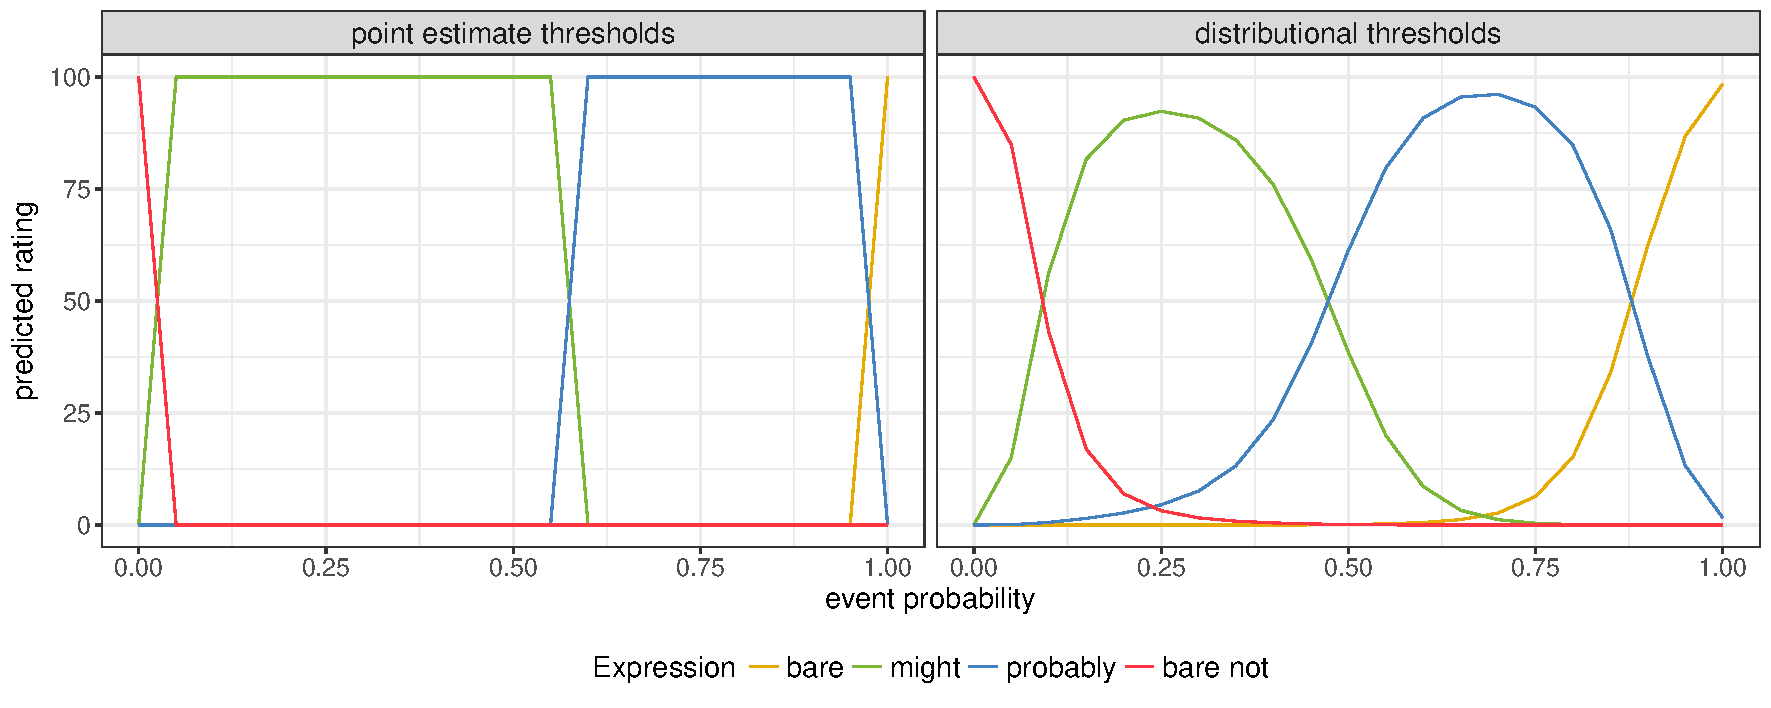
\includegraphics[width=\textwidth]{plots/model-visualization-predictions.pdf}

\caption{Example threshold distributions (upper panels) and corresponding model predictions for the \textit{expected pragmatic speaker} model (lower panels). In this example, the set of possible utterances is $U=\{$\textsc{bare}, \textsc{might}, \textsc{probably}, \textsc{bare not}$\}$, all utterances have equal costs, the rationality parameter $\lambda$ is set to 10, and the prior probability over event probabilities $P(\phi)$ is a uniform distribution. As the panels on the left show, point estimates of thresholds lead to sharp categorical boundaries in the model predictions, whereas distributions over thresholds, as in the panels on the right, lead to gradually increasing and decreasing predicted utterance ratings. \label{fig:model-visualization}}
\end{figure}



$S_1$ crucially depends on a vector of thresholds $\theta$ which contains a threshold for each uncertainty expression in the utterances in $U$, 
as well as a cost function $c(u)$. The values that participants expect a \textit{pragmatic speaker} to assign 
to these variables are unknown a priori; we infer these values from the data collected in the above reported experiment. 
In Experiment~1, we found that both at the population level and at the individual level, 
participants' ratings of the different expressions gradually increased and decreased with changing event probabilities 
(as, for example, shown in Figure~\ref{fig:norming-results-indiv}). This is expected if participants
have probabilistic beliefs about thresholds $\theta$ (as illustrated in the right panels of Figure~\ref{fig:model-visualization}) but not if they reason based on point estimates of $\theta$ (as illustrated in the left panels of Figure~\ref{fig:model-visualization}).
Considering these observations,  we assume that listeners hold beliefs about a speaker's thresholds in the form of a distribution $P\left(\theta_e\right)$.\footnote{We leave it open 
whether a {speaker} samples from a distribution over thresholds when producing utterances (as suggested by \textcite{Qing2015}) 
or always uses the same values for thresholds. In the former case, listeners could have higher-order beliefs  $P(\eta)$ 
about different {speakers}' threshold distributions instead of having direct beliefs about the thresholds that different 
{speakers} use. For our purposes, this distinction does not matter since we assume that listeners would marginalize over higher-order beliefs $P(\eta)$ such that  $P\left(\theta_e\right) = \int P\left(\eta\right) P\left(\theta_e \mid \eta\right) d\eta$ and we therefore take the simplest approach and directly model $P\left(\theta_e\right)$. } Analogously, we assume that  listeners also have beliefs $P(c)$ about the speaker model's cost function.
Using these two distributions, we can define the \textit{expected pragmatic speaker} model $ES_1\left(u_e \mid \phi \right)$ as follows:

$$ES_1\left(u_e \mid \phi \right) = \int P(c) \int_0^1 P(\theta) S_1\left(u _e\mid \phi, \theta, c\right) d\theta \  d c$$

This model predicts which utterance listeners with uncertainty about a speaker's thresholds and cost function would expect that {speaker} to use to describe different event probabilities. 
Intuitively, this model can be seen as a weighted average of different \textit{pragmatic speaker} models, where individual models differ in terms of thresholds and cost functions.  The weights of this average are determined by listeners' belief distributions over thresholds and costs. For example, if listeners believe that it is likely that a speaker uses a threshold $\theta_{probably}$ of 0.5, they will assign higher weight to speaker models
using this threshold than models using other thresholds. 

%$P(\theta)$ serves two purposes here: On the one hand, it captures the variability in expectations across participants and on the other hand, it captures individual participants' uncertainty. 
%In theory one could separate these two distributions by having one distribution modeling the variability across participants and then having a separate distribution for each listener capturing
%their uncertainty. Since we are primarily concerned with modeling population-level expectations in this work, we decided to conflate these two source of variability.


%\textbf{TODO:} walk through example model and show how this model is capable of pragmatic inferences and different preferences

\subsection{Linking function}

We assume that in Experiment~1, participants, when asked to provide ratings for utterances, reasoned about a generic speaker's 
likely descriptions of varying event probabilities. 
We assume that this reasoning was guided by participants' beliefs about the speaker's thresholds and costs, and 
that participants averaged over their uncertainty. For this reason, we assume that the population-level 
average ratings of what participants expect the speaker to say in different situations 
correspond to the probabilities predicted by the \textit{expected pragmatic speaker} model (with the \textit{something else}
option being predicted by the sum of the probabilities of all utterances not present in a condition; see below for more details).
Further, given the forced choice nature of the experiment and that we estimate model 
parameters from limited and potentially noisy data, we make the following additional linking assumptions
for which we provide a rationale and an assessment of their importance in turn.

\begin{itemize}
\item \textbf{Set of utterances}: Across all conditions, we assume that the set of utterances that participants are 
considering is the set of all utterances that we used in Experiment~1, i.e., $U= \{$ \textsc{bare}, \textsc{might}, 
\textsc{probably}, \textsc{think}, \textsc{looks like}, \textsc{could}, \textsc{bare not}$\}$. We include all utterances 
instead of only the utterances that are presented in a given condition since we assume that participants' general 
knowledge of English uncertainty expressions also influences their ratings. Ideally, we would include even more 
utterances in this set of alternatives but since we can only estimate parameters for uncertainty expressions for 
which we collected ratings, we are limited to the utterances in $U$. 

The exact set of utterances is not that important for fitting the data as long as the set includes the \textsc{bare}
and \textsc{bare not} utterances as well as at least one utterance with a weaker 
(e.g., \textit{might}) and one with a stronger (e.g., \textit{probably})
uncertainty expression.

\item \textbf{\textit{something else} option}: Participants in condition $\mathscr{C} = \{u_a, u_b\}$ 
could only choose between the three utterances $U' = \{u_a, u_b,$ \textit{something else}$\}$.
For modeling data from condition $\mathscr{C}$, we therefore need a function to predict the ratings 
for the utterances in $U'$. For $u_a$ and $u_b$, this is straightforward: We assume the probability 
of a participant choosing $u_a$ or $u_b$
is proportional to $ES_1(u_a \mid \phi)$ and $ES_1(u_b \mid \phi)$, respectively. 
We model the probability of a participant choosing the \textit{something else} option as the sum 
of the probability of all utterances that were not part of the condition as well as a constant $O$, 
which accounts for probability mass assigned to utterances that participants might be 
considering but which are not contained in $U$. This gives us the following condition-specific 
function $ES_1^{(\mathscr{C})}$ for predicting participants' ratings.

$$
ES_1^{(\mathscr{C})}(u \mid \phi) \propto 
    \begin{cases}
      ES_1(u \mid \phi) & \quad\mbox{if } u  \in \mathscr{C}\\
       O + \sum_{u \not \in \mathscr{C}} ES_1(u \mid \phi) & \quad \mbox{if $u$ is \textit{something else}} \\
   \end{cases}
$$

This summation over alternative utterances is crucial for fitting the data since we need to
capture the ratings for \textit{something else}. The only viable alternative would be
to fit individual curves for \textit{something else} for each condition, which would require
the estimation of considerably more parameters and would not explain the ratings for the
\textit{something else} option. The inclusion of the constant $O$ is less important but it
still improves model fit.


\item \textbf{Cost function}: We assume that the cost function represents participants' beliefs about the speaker's 
preferences for different utterances. Lower costs of an utterance indicate higher speaker preferences. We further 
assume that we are cueing participants to believe that the speaker would be likely to use the two utterances, $u_a$ 
and $u_b$, that are provided in condition $\mathscr{C}=\{u_a, u_b\}$ and that participants therefore primarily use the 
\textit{something else} option when both of the two utterances are semantically infelicitous or otherwise highly unexpected. 
We model this cueing effect in our choice of the cost function $c(u)$, which depends on the condition. For the two utterances 
that are presented to the participants, we set the cost to $1$ and for all the other utterances, we set the cost to a constant $\gamma > 1$:
$$
c(u, \mathscr{C}) = 
     \begin{cases}
       1 &\quad\text{if } u  \in \mathscr{C}\\
       \gamma &\quad\text{otherwise} \\
     \end{cases}
$$

Theoretically, we could have also used a different constant $\gamma_u$ for each utterance. The data from
Experiment~1, however, suggests that participants generally did not prefer one utterance over 
the other. To limit the number of free model parameters and to prevent overfitting, we therefore use a single
constant $\gamma$ for all utterances. We will, however, relax this assumption in our adaptation model in \sectionref{sec:model-adapt}, which
we use to investigate whether listeners update their beliefs about preferences during adaptation.

This condition-specific cost function is important for the model fit. If we didn't use such a cost function, 
the model would assign much higher ratings to the \textit{something else} option than participants did.

\item \textbf{Noise}: Finally, to account for participants not paying attention or making mistakes, 
we also include a noise term that models participants providing random ratings.
The amount of noise is captured by the noise strength parameter $\delta$. This parameter
indicates the proportion of random responses, that is, the proportion of responses drawn from a uniform distribution
over the three condition-specific responses $U'$. 

The inclusion of the noise term is not crucial for fitting the data but it does improve model fit and
is common practice in RSA models whose parameters are estimated from experimental data \parencite[see][]{Herbstritt2019,Tessler2019}.

\end{itemize}

\noindent Incorporating all of these assumptions, we end up with the following noisy, condition-specific expected pragmatic speaker 
model $ES_1^{(\mathscr{C})'}(u \mid \phi)$, which we use to predict participants' ratings:

$$ES_1^{(\mathscr{C})'}(u \mid \phi) = \delta \times \frac{1}{|U'|} +  (1 - \delta) \times ES_1^{(\mathscr{C})}(u \mid \phi)$$

For the prior distribution over event probabilities $P(\phi)$, which is used in the literal listener model $L_0$, 
we use a uniform distribution over the interval $[0,1]$.\footnote{To 
verify the assumption that the prior on event probabilities is uniform, we conducted a separate norming study in which participants rated 
how likely they thought it was that a speaker described different gumball machines containing different 
proportions of blue and orange gumballs after hearing an unintelligible utterance. We found that on average 
participants rated all gumball machines equally likely which suggests that the prior over event probabilities is 
indeed uniform.} For the distributions over thresholds $P(\theta_e)$, we use a Beta distribution parametrized by 
$\alpha_e$ and $\beta_e$. The choice of Beta distributions is motivated by two of its properties. First, the support of a Beta distribution 
is the interval $[0,1]$ which corresponds to the exact range of possible values for $\theta_e$.

The second reason for using Beta distributions is that, depending on the parameterization, 
Beta distributions can take on very different shapes. This property is important because we are making
the simplifying assumption that all utterances in our experiments have a threshold semantics.
Such a semantics is commonly assumed for uncertainty expressions such as \textit{probably} \parencite[e.g.,][]{Yalcin2010,Lassiter2016}, 
but it is unconventional for bare assertions such as \textit{``You'll get a blue one''}, which are generally assumed to be  
true only if the event is certain to happen, i.e., it has an event probability of 1. However, since Beta distributions can have a shape 
like the distribution for \textsc{bare} in the upper right panel in Figure~\ref{fig:model-visualization}, the model has the capability to infer
a semantics for the bare form that is almost equivalent to a traditional semantics of bare assertions. In this parameterization of the
Beta distribution, most probability mass is assigned to values of $\theta$ close to 1, which is mathematically almost equivalent to
a traditional semantics.\footnote{Alternatively, one can also see the threshold distribution for the bare form as a distribution over a verification parameter $\eta$ that governs 
how certain a speaker has to be to utter a bare assertion \parencite[see, e.g.,][]{Moss2018}. Mathematically, our assumption of bare forms having a threshold
semantics is equivalent to assuming that bare assertions are only true when a speaker's credence of the proposition exceeds the verification threshold $\eta$.}
Therefore, using Beta distributions for the threshold distributions has the desirable effect of allowing us a unified treatment of all expressions included in the model. 

\subsection{Parameter estimation}

Given all the assumptions outlined above, the model has  $18$ parameters in total: A cost parameter $\gamma$, a rationality parameter $\lambda$, a noise strength parameter $\delta$, a constant corresponding to other utterances $O$, and for each utterance, Beta distribution parameters $\alpha_e$ and $\beta_e$. We estimated these parameters jointly from all 21 conditions of Experiment~1 using Bayesian data analysis \parencite[BDA; see, e.g.,][]{Kruschke2015}. To construct the dataset, we treated the ratings by each participant as a probability distribution from which we sampled 10 utterances. We used highly uninformative
uniform priors over the interval $[0,15]$ for the Beta distribution and cost parameters, uniform priors over the interval $[0,7]$ for the rationality parameter, and uniform priors over the interval $[0,0.5]$ for $O$ and the noise strength parameter. We estimated the vector of parameters $\Theta$ using MCMC with a Metropolis Hastings sampler. To decrease autocorrelation of the chain, we collected a sample only at every 10th iteration (i.e., we use thinning of 10). We discarded the first 10,000 burn-in samples and then collected 50,000 samples.  We ran four MCMC chains and confirmed convergence by computing the $\hat{R}$-statistic \parencite{Gelman2003}. More details on the implementation of the model can be found in Appendix C.

\subsection{Model evaluation}



\begin{figure}[th!]
\includegraphics[width=\textwidth]{plots/pre\string_test\string_model\string_main.pdf}
\caption{Model predictions and results from Experiment~1. Error bars correspond to 95\% high density intervals (model predictions) and bootstrapped 95\%-confidence intervals (observed results). \label{fig:norming-results-model-main}}

\end{figure}


The result of the parameter estimation procedure is a posterior distribution over parameters given the observed data $P(\Theta \mid D_{obs})$. We evaluated
 model fit by performing a posterior predictive check \parencite[PPC;][]{Kruschke2015}. To this end, we took 10,000 samples of parameters $\Theta$ from the posterior distribution. For each sample, we computed the model predictions $ES_1^{(\mathscr{C})'}(u \mid \phi)$ parameterized by $\Theta$. We then compared the average model predictions to the
mean ratings that participants had provided in the pre-exposure experiments. We further computed the 95\% high density interval  \parencite[HDI;][]{Kruschke2015} which reflects the ctertainty of the model
about its predictions.

Figure~\ref{fig:norming-results-model-main} shows the model predictions and the experimental data for three conditions 
(see Table~\ref{tbl:correlations} and Appendix~D for modeling results for all 21 conditions). As these plots show, the model
is able to capture almost the entire variance in participants' average ratings. Further, the 95\% HDIs are very small, which suggests
that the model is certain about its predictions. Both of these observations are also true for the model's predictions for all the other
conditions. For 19 of the 21 conditions, the $R^2$ value between the model predictions and the experimental data exceeds 0.9,
and for the remaining 2 conditions, the $R^2$ value exceeds 0.88. 

Most cases in which the model predictions and the experimental data deviate concern the ratings at the two extremes of the event probability space.
The model often underpredicts ratings for the \textit{something else} option when there is either a 0\% or a 100\% chance of 
getting a target color gumball. In these situations, participants presumably thought that {\sc bare} and {\sc bare not} are the most appropriate
utterances and therefore rate \textit{something else} highly unless we provide them with the {\sc bare} or {\sc bare not} options. The model predicts
this behavior to some extent but seems to assume that participants were cued more heavily towards the presented utterance options than they actually were.
This could be an indicator that we should revisit our unconventional approach of treating the bare forms like uncertainty expressions with a threshold semantics,
since the model would predict higher ratings for \textit{something else} at both ends of the scale if we assumed that the bare form and its negation were only true
in the cases of 100\% and 0\% event probabilities, respectively. 
However, for our purposes in this paper, the exact predictions about production choices for objectively certain events are not as important and hence
we decided against revising the assumption that all utterances in the model have a threshold semantics.

The comparably low $R^2$ for the \textit{probably-think} condition ($R^2=0.88$) stems
from the fact that participants disagreed on the ordering of these two expressions. This  
led to a bimodal distribution of average ratings (see the figure in Appendix~B) for \textsc{think}, which our population-level 
model cannot fully capture. This suggests that if we wanted to perfectly model participants' production expectations, we should
additionally model participant-level differences. However, since the ordering of \textit{probably} and \textit{think} is not of great relevance
for our investigation of adaptation to different uses of \textit{might} and \textit{probably}, we did not attempt to fit a more complex model
that can account for individual listener differences. 

One potential concern given the flexibility of the model is that it could be overfitting the data. 
This is unlikely considering that all parameters are shared across all conditions and thus we are estimating only 18 parameters to predict in total 567 data points 
(27 data points for each one of the 21 conditions). To nevertheless rule out the possibility of overfitting, we performed a leave-one-out cross-validation of
the model. For each condition $x$, we estimated a distribution over parameters $\Theta_x$ using the data from all conditions but $x$. We then
compared the model predictions of the model parametrized by $\Theta_x$ to participants' ratings in condition $x$. This way, the model has to predict
participant behavior which it has not observed during parameter estimation. Table~\ref{tbl:correlations} shows the $R^2$ values for participants's
ratings and model predictions for the model estimated from all conditions and the leave-one-out models.

\begin{table}[ht!]
\center
\begin{tabular}{l | c | c}
      Condition & $R^2$ (all data) & $R^2$ (leave-one-out) \\
      \midrule
          bare-might  &  0.992  & 0.988 \\
       bare-probably  &  0.978  & 0.976 \\
          bare-could  &  0.978  & 0.976 \\
     bare-looks like  &  0.927  & 0.896 \\
          bare-think  &  0.968  & 0.964 \\
      might-probably  &  0.964  & 0.954 \\
         might-could  &  0.921  & 0.910 \\
    might-looks like  &  0.934  & 0.918 \\
         might-think  &  0.946  & 0.934 \\
      probably-could  &  0.961  & 0.959 \\
 probably-looks like  &  0.944  & 0.931 \\
      probably-think  &  0.888  & 0.860 \\
    could-looks like  &  0.924  & 0.910 \\
         could-think  &  0.931  & 0.920 \\
    looks like-think  &  0.970  & 0.960 \\
       bare not-bare  &  0.894  & 0.848 \\
      bare not-might  &  0.968  & 0.958 \\
   bare not-probably  &  0.910  & 0.893 \\
      bare not-could  &  0.910  & 0.840 \\
 bare not-looks like  &  0.927  & 0.903 \\
      bare not-think  &  0.933  & 0.920 \\
\end{tabular}
\caption{$R^2$ values for experimental data and model predictions for model estimated from all data and for models estimated from all conditions except the predicted condition. \label{tbl:correlations}}
\end{table}


As this table shows, the $R^2$ values remain high\footnote{\add{We only observed slightly bigger drops in correlations for the \textit{bare not-bare} and the \textit{bare not-could} conditions. In these conditions, we paired expressions that are a poor description for a large range of event likelihoods: \textsc{bare not} and \textsc{bare} are only expected to be good descriptions if the event probability is very low or very high, respectively, and the \textit{bare not-could} condition  includes expressions of which neither are well suited to describe high event probabilities. As a result, participants in these conditions seemed to be more uncertain what to do which was reflected in several participants commenting in a post-experiment survey that they would have answered differently had there been better response options. Participants' ratings were therefore presumably more idiosyncratic, which made it harder for the model to predict ratings without having access to the data from these conditions.}} even if we exclude the data on which the model is evaluated from the model's training data, 
which suggests that our proposed model indeed explains
participants' expectations of a generic speaker's uncertainty expressions. 

\begin{figure}[th!]
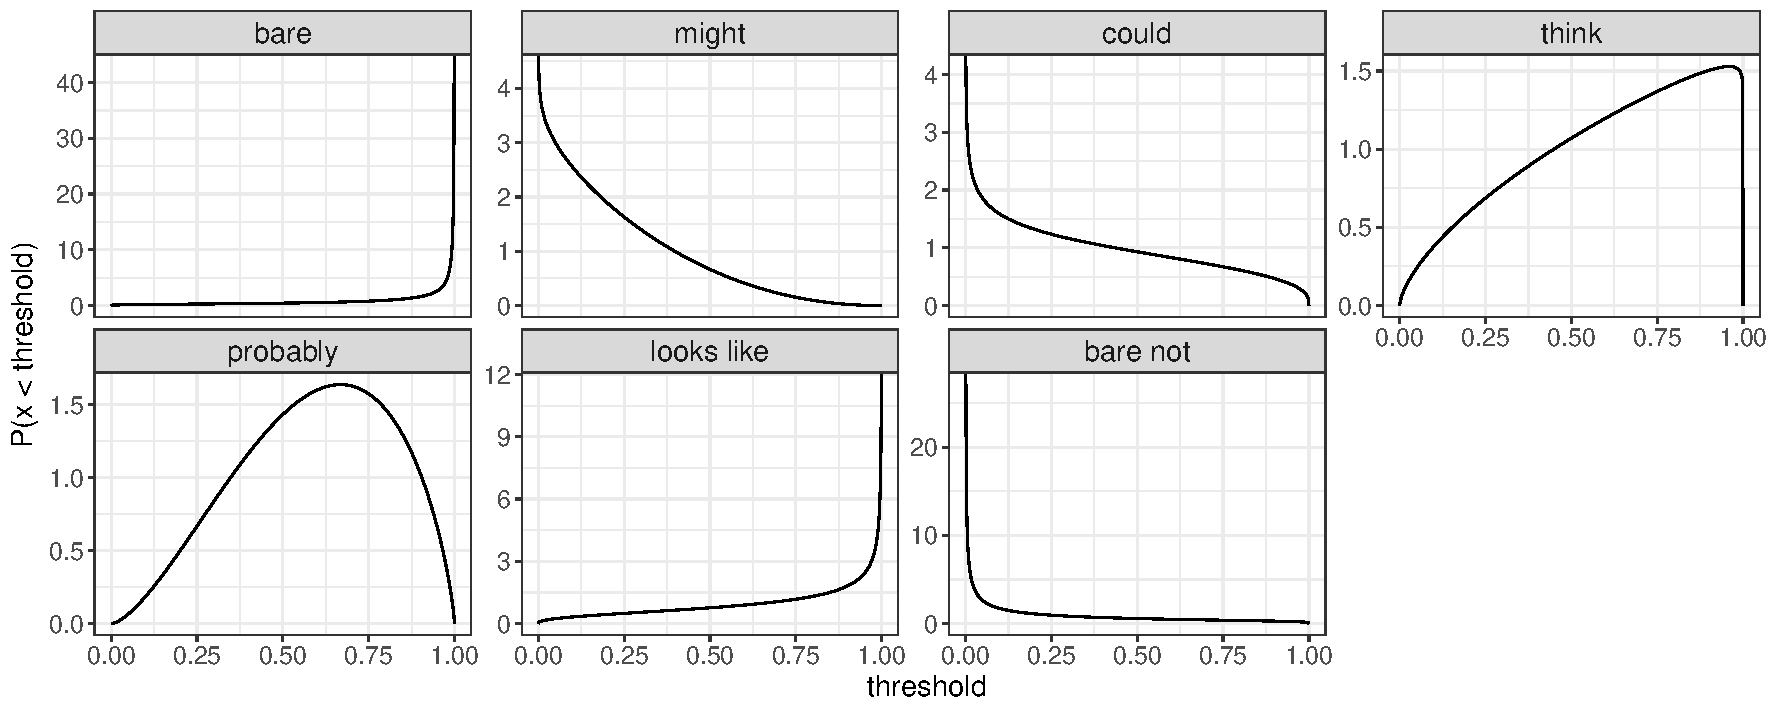
\includegraphics[width=\textwidth]{plots/threshold-distributions-prior.pdf}
\caption{Inferred threshold distributions. For the negative bare utterance (\textsc{bare not}), the distribution is over an upper threshold, i.e., a bare statement embedded under negation is true if the probability of the event is lower than the threshold. For all other utterances, the distribution is over a lower threshold. 
\label{fig:threshold-distributions}}
\end{figure}

Lastly, one of the advantages of Bayesian cognitive models is that their parameters are interpretable. Figure~\ref{fig:threshold-distributions} shows the 
maximum likelihood estimates of the inferred threshold distributions $P(\theta)$ for the seven uncertainty expressions that we included in our experiments.
The first observation is that most threshold distributions have considerable variance rather than being peaked at a particular value. This suggests that
listeners have probabilistic beliefs -- i.e., uncertainty -- about the semantic threshold for each utterance.

Further, the inferred threshold distributions are broadly in line with qualitative accounts of the meaning of uncertainty expressions.
As discussed above, for the bare form and its negation, we expected the model to infer threshold distributions whose probability mass is concentrated 
around $\theta=1$ and $\theta=0$, respectively.\footnote{Note that since the negation of the bare form is a negative form, $\theta$ is an upper threshold. For the bare form as well as
all the other utterances that we are are considering in this paper, $\theta$ is a lower threshold.} As  Figure~\ref{fig:threshold-distributions} shows, this is indeed what
the inferred threshold distributions look like. 

The probability mass of the threshold distribution for \textit{might} is  concentrated at values slightly above 0. This, too, 
is in line with non-probabilistic accounts of the interpretation of epistemic modals. These accounts generally assume that \textit{might} $p$ is true 
if there exists a world $w$ in a set of (contextually restricted) epistemically accessible worlds $E$ such that $p$ is true in $w$ 
\parencite[e.g.,][]{Kratzer1991,Swanson2008,Hacquard2011}. One way to translate this logical condition into our probabilistic framework is to assume that 
in our gumball machine context, there exists an epistemically accessible world $w$ for each gumball $g$ and that in world $w$, one gets gumball $g$. 
Under this assumption, \textit{``You might get a blue gumball''} is true if there exists an epistemically accessible world $w$  in which one gets a
gumball $g$ that is blue. At the same time, if such a world exists, then $P(\mbox{blue gumball})$ is greater than 0, which approximately corresponds
to the threshold semantics with the inferred threshold distribution of the model. The inferred threshold distribution for \textit{could} is very similar, 
but not identical, to the one of \textit{might}. This also largely reflects the prediction by non-probabilistic accounts, which generally assume that \textit{might} and epistemic 
\textit{could} are semantically equivalent \parencite{Kratzer1991,Hacquard2011}, but it also suggests that there are differences between these two expressions. 

The threshold distribution for \textit{probably} has most of its probability mass concentrated at thresholds above 0.5. This again largely reflects the predictions of 
existing accounts that assume that \textit{probably} $p$ is true if $p$ is more likely than the negation of $p$ \parencite[e.g.,][]{Kratzer1991}. However, it is also noteworthy that the inferred
distribution has some probability mass below 0.5, which potentially provides evidence for theoretical arguments by \textcite{Yalcin2010} that \textit{probably} $p$ can
sometimes also be true if $p$ is less likely than the negation of $p$.\footnote{Since we did not investigate whether participants always 
correctly perceived the event likelihood to be less than 0.5 for gumball machines with less than 50\% target color gumballs, an alternative explanation for this observation would be that participants sometimes overestimated the event likelihood and for this reason, they expected the generic speaker to use \textit{probably} despite an objective event likelihood of less than 0.5.}

The threshold distributions for the remaining expressions, \textit{looks like} and \textit{think} also match intuitions. The distribution for 
\textit{looks like} has most of its probability mass near threshold values of 1 but is overall slightly weaker, i.e., assigns higher probabilities to lower thresholds,
than the bare form. The distribution for \textit{think} assigns most probability mass to high thresholds, which is compatible with the intuition
that speakers use \textit{think} when they strongly believe the embedded proposition but are not entirely certain that it is true.
 
 
 \begin{table}[ht!]
\center
\begin{tabular}{l | c | c | c | c }
     & $\lambda$ (rationality) & $\gamma$ (cost) & $\delta$ (noise) & $O$ (other utterances) \\
      \midrule
      MAP & 2.21 & 3.03 & 0.074 & $3.64 \times 10^{-5}$ \\
      CI & [2.16, 2.26] & [2.98, 3.08] &  [0.069, 0.079] &[$2.89 \times 10^{-5}$, $4.50  \times 10^{-5}$] \\
      
         \end{tabular}
\caption{Estimated maximum a posteriori estimates (MAP) and 95\% credible intervals (CI) for model parameters. \label{tbl:model-params}}
\end{table}

  \tableref{tbl:model-params} shows the MAP values and credible intervals for the remaining parameters. The model inferred that speakers
  are relatively likely to choose an optimal utterance (reflected in the $\lambda$ parameter being
  greater than 1); that utterances that are not included in the experiment incur a considerable cost  (reflected in the $\gamma$ parameter being greater than 1); that about 7.4\%
  of the data should be treated as noise (reflected in the $\delta$ parameter); and that the production probability of utterances not included in our set of utterances is low. 

 
 \subsection{Interim summary}
 
 In this section, we described a computational model of production expectations of uncertainty expressions. This model
 is couched within the RSA framework and assumes that listeners hold beliefs about a speaker's lexicon (in the form
 of utterance-specific threshold distributions) and about speaker preferences (in the form of utterance-specific costs). We estimated 
 the free parameters of this model from the results of Experiment~1, which resulted in a model that is able to accurately predict
 participants' utterance ratings -- i.e., their expectations of use --  in Experiment~1 across all conditions with a shared set of parameters.
 
 In the following sections of this paper, we will use this model as the basis for modeling adaptation. Since this model
 is able to capture different beliefs about thresholds and preferences, it provides us with the opportunity to simulate 
 the adaptation process as a result of updating beliefs about these model parameters. Further, in order to answer
 our primary research question of whether listeners update their beliefs about lexica or preferences, we compare
 different adaptation simulations in which we allow different types of parameters to be updated.





\section{Experiment 2: Adaptation of speaker expectations}
\label{sec:exp-prod-adaptation}

We now turn to our main research questions of whether and how listeners adapt to variable uses of uncertainty expressions.
In Experiment~1, we found that participants show uncertainty in their expectations about a generic speaker's 
use of \textit{might} and \textit{probably}. Based on these results, we investigate whether participants
form speaker-specific expectations about the use of \textit{might} and \textit{probably} after observing a specific speaker's use of 
uncertainty expressions for a short period of time. The procedure, materials and analyses were pre-registered at \url{https://osf.io/w926x/}.\footnote{This experiment is a follow-up to a previous experiment with a potential confound due to different number of exposures across conditions. See Appendix~E for a discussion of the previous experiment. The qualitative results of both experiments are identical.}


\subsection{Method}

\subsubsection{Participants}
We recruited a total of 80 participants (40 per condition) on Amazon Mechanical Turk. 
We required participants to have a US-based IP address and a minimal approval rating 
of 95\%. Participants were paid \$2.20 which amounted to an hourly wage of approximately 
\$12--\$15. None of the participants participated in Experiment~1.

\subsubsection{Materials and procedure}

\paragraph{Exposure trials:} In the first part of the experiment, participants saw 25 exposure trials. 
These trials had a similar setup as the trials in Experiment~1: 
they also showed a child requesting a blue or orange gumball and a gumball machine with blue and orange gumballs. 
However, instead of the cartoon adult, they showed a video of an adult male or female speaker (counterbalanced across participants) producing one of the following six utterances:

\begin{itemize}
\item You'll get a blue/orange one (\textsc{bare})
\item You might get a blue/orange one (\textsc{might})
\item You'll probably get a blue/orange one (\textsc{probably})
\end{itemize}

\begin{table}
\centering
\begin{tabular}{l c c c c c c}
\toprule
& \multicolumn{2}{c}{\sc might} & \multicolumn{2}{c}{\sc probably} & \multicolumn{2}{c }{\sc bare}  \\
& $n$ & $\phi$ & $n$ & $\phi$ & $n$ & $\phi$ \\
\midrule
\emph{cautious} & {\bf 10} & {\bf 60\%} & 10 & 90\% & 5 & 100\%  \\
\emph{confident} & 10 & 25\% & {\bf 10}  & {\bf 60\%} & 5  & 100\%  \\  
\bottomrule
\end{tabular}

\caption{Number of exposure trials ($n$) per utterance ({\sc might}, {\sc probably}, {\sc bare}) 
and associated proportion of target color gumballs ($\phi$) in the \emph{cautious} vs.~\emph{confident} 
speaker conditions in Experiment 2. Critical trials bolded. \label{tbl:materials}}

\end{table}

The number of trials with each of these utterances as well as the gumball proportions varied across two conditions (see Table \ref{tbl:materials} for an overview). In the {\it confident speaker} condition, participants saw 10 critical trials with 60\% target color gumballs and the speaker producing an utterance with \emph{probably} (target color was randomized across trials), 5 filler trials with 100\% target color gumballs and the speaker producing {\sc bare}, and 10 filler trials with 25\% target color gumballs and the speaker producing {\sc might}. In the {\it cautious speaker} condition, participants saw 10 critical trials with 60\% target color gumballs and the speaker producing an utterance with \emph{might}, 5 filler trials with 100\% target color gumballs and the speaker producing {\sc bare}, and 10 filler trials with 90\% target color gumballs and the speaker producing {\sc probably}. The filler trials contained utterance-event probability pairs that were rated very highly in the \textit{might-probably} condition of Experiment~1 (see \figref{fig:norming-results-main}) and were intended to boost confidence in the speaker.

Participants were instructed to watch what the speaker had to say to the child. The video started automatically after a 400ms delay and participants had the option to replay the video as often as they wanted. To advance to the next scene, participants had to press a button which was disabled until the video clip had finished.

\paragraph{Test trials:} The test phase was almost identical to the  \textit{might-probably} condition of Experiment~1 except that the cartoon figure of the man was replaced with a picture of the speaker that participants saw on the exposure trials. Participants were presented with scenes containing gumball machines with 9 different proportions of blue and orange gumballs  (identical as in Experiment~1) and they were asked to provide ratings for the utterances {\sc might} and {\sc probably} by distributing 100 points across these two utterances and the blanket {\it something else} option. Participants provided two ratings for each of the 18 color-gumball machine combinations resulting in a total of 36 trials. 

Both speakers were from the East Coast and Native Speakers of North American English.
%\footnote{The first author compensated each of the speakers for their help with the recordings with two slices of marble Guglhupf.} 
They were instructed to produce the utterances in a normal voice without any special prosody. The speakers were
na\"ive to the purpose of the experiment.


\paragraph{Attention checks:}  In order to verify that participants were paying attention to the video and the scenes, we included 15 attention checks (6 during exposure and 9 during test trials), which were randomly positioned within the two experimental phases. Trials that contained an attention check either displayed or did not display (pseudo-randomized) a small grey X somewhere around the gumball machine. After completing a trial with an attention check, participants were asked whether they had seen a grey X in the previous scenes or not.

\subsubsection{Exclusions} We excluded participants who provided incorrect responses to more than 3 of the attention checks. Based on this criterion, we excluded 8 participants in the \textit{cautious speaker} condition, and 7 participants in the \textit{confident speaker} condition. None of the results reported below depend on these exclusions.


\subsubsection{Analysis and predictions}  

Intuitively, we expect a more confident speaker to use lower thresholds for {\it probably} and {\it might} than a more cautious speaker.
Therefore, if participants track these different uses, we expect their ratings to depend on how the speaker used uncertainty expressions during the exposure phase. 
Concretely,  in our forced choice production paradigm, we expect participants in the \textit{confident speaker} condition to rate {\sc probably} highly for a larger range of event probabilities than participants
in the \textit{cautious speaker} condition. 
Following \cite{Yildirim2016}, we quantified this prediction by fitting a spline with four knots for each expression and each participant and computing the area 
under the curve (AUC) for the splines corresponding to each expression and participant. The area under the curve is proportional to how highly and for how large 
of event probabilities participants rate an utterance. If an utterance is rated highly for a larger range of event probabilities, the AUC will also be larger. 
We therefore tested whether listeners updated their expectations according to these intuitions by computing the difference between the AUC of the spline for 
{\sc might} and of the spline for {\sc probably} for each participant. We predicted that the mean AUC difference would be larger in the 
\emph{cautious speaker} condition than in the \emph{confident speaker} condition.

\subsection{Results and discussion}

\begin{figure}
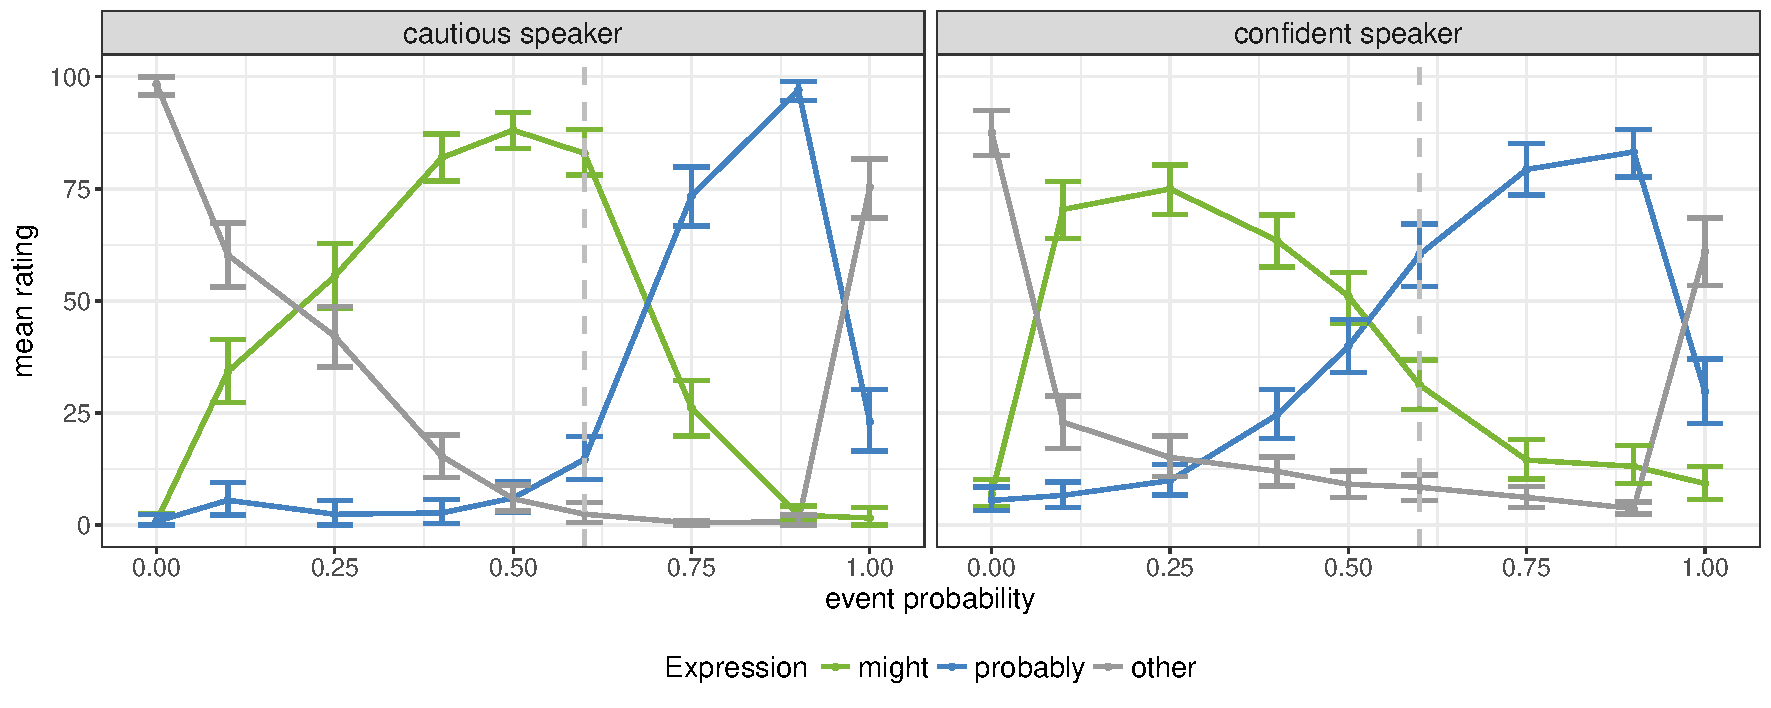
\includegraphics[width=\textwidth]{plots/exp-1-replication-ratings.pdf}
\caption{Mean ratings for the \textit{might-probably} condition from Experiment 1 (repeated from \figref{fig:norming-results-main}) and mean post-exposure ratings from Experiment~2. Error bars correspond to bootstrapped 95\%-confidence intervals.  The grey dotted line highlights the ratings for the 60\% event probability ratings.  \label{fig:adaptation-results-prod}}
\end{figure}

\begin{figure}
\center
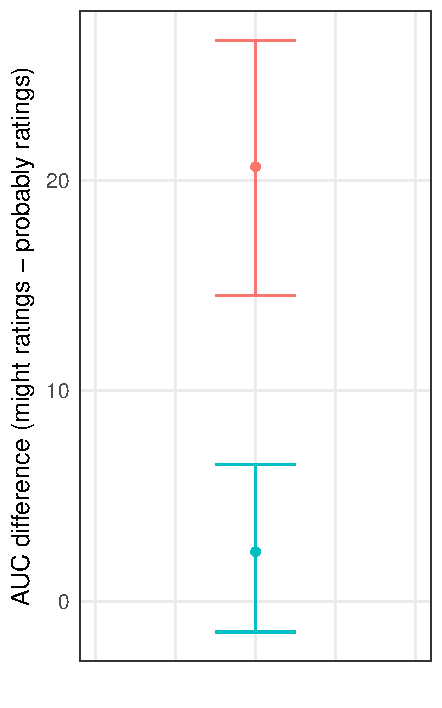
\includegraphics[width=.4\textwidth]{plots/exp-1-auc.pdf}
\caption{Area under the curve (AUC) differences from Experiment~2. Error bars correspond to bootstrapped 95\%-confidence intervals.  \label{fig:adaptation-auc-prod}}
\end{figure}

The center and right panels of Figure~\ref{fig:adaptation-results-prod} show the mean ratings for the three options in the two conditions. As these plots show, participants updated their expectations about the speaker's language use, and therefore made different predictions about how the speaker would use uncertainty expressions as compared to prior expectations elicited in Experiment~1 (left panel). In the \emph{cautious speaker} condition, participants gave high ratings for {\sc might} for a larger range of event probabilities than in the \emph{confident speaker} condition. On the other hand, participants gave high ratings for {\sc probably} for a larger range of gumball proportions in the \emph{confident speaker} condition than in the \emph{cautious speaker} condition. These differences result in a significantly larger AUC difference in the \emph{cautious speaker} condition than in the \emph{confident speaker} condition ($t(63) = 2.99$, $p < 0.01$, see also Figure~\ref{fig:adaptation-auc-prod}).

As Figure~\ref{fig:adaptation-results-prod} shows, participants also differed in their ratings of the two utterances when they were presented with a scene with 60\% target color gumballs. In Experiment~1, participants assigned approximately equal ratings to both expressions; in the \emph{cautious speaker} condition, participants rated {\sc might} higher than {\sc probably}; in the \emph{confident speaker} condition, the pattern was reversed and participants rated {\sc probably} higher than {\sc might}. These expectations mirror the speaker behavior during the exposure phase and provide additional evidence that participants tracked the speaker's usage of uncertainty expressions. 

%Our results also seem to rule out an alternative explanation according to which participants were inferring higher-level speaker goals rather than forming expectations about the speaker's language use. For example, prima facie, it could be that participants inferred that the  \textit{confident speaker} wanted to appear encouraging towards the child. However, if participants inferred such a higher-level goal, then we would expect participants to belief that the speaker would use utterances that are even more encouraging when there is a high probability of getting a target color gumball, resulting in higher ratings of the \textit{something else} option for high event probabilities. We did not observe such an effect, and  in fact, numerically, the rating of \emph{something else} was higher in the \emph{cautious speaker} condition than in the \textit{confident speaker} condition.

The results further suggest that participants updated their mappings between uncertainty expressions and event probabilities: In the {\it confident speaker} condition, {\sc might} and {\sc probably} were rated highly for lower event probabilities than in the {\it cautious speaker} condition. This experiment further provides evidence against an account according to which participants only learn that the \emph{cautious speaker} prefers to use {\sc might} and the {\it confident speaker} prefers {\sc probably}. Since the frequency of both expressions was the same in this experiment, participants could not have inferred a preference for one of these two utterances. 

%That we nevertheless observed different ratings in the two speaker conditions suggests that participants updated their beliefs about the mapping between expression and event probabilities.

In sum, the results from this experiment provide evidence for listener adaptation to a specific speaker's use of uncertainty expressions after a brief exposure phase. Further, the results 
suggest that listeners' expectations about a speaker's language use are at least not exclusively driven by tracking speakers' preferences for different utterances. We investigate the nature of the updated expectations
in the next section.


%However, one potential confound in this experiment is that the number of utterances with \textit{might} and \textit{probably} differed across the two conditions (see left part of Table~\ref{tbl:materials}). It is possible that participants only learned that the {\it cautious speaker} overall prefers to use {\sc might} and the {\it confident speaker} prefers {\sc probably}. To address this confound, we conducted another experiment in which we balanced the number of exposures to {\sc might} and {\sc probably}.

\section{Adaptation model}
\label{sec:model-adapt}



The experimental results presented in the previous section suggest that listeners update
\textit{some} expectations about language use when they interact with a speaker. 
However, the nature of the updated representations is unclear. As mentioned in the introduction, there are three likely candidates:
first, it is possible that listeners update their expectations about the speaker's lexicon 
(i.e., the mapping between event probabilities and uncertainty expressions);  second, listeners
 might  update their expectations about the speaker's preferences; 
and third, they might update both their expectations about the speaker's lexicon 
and about the speaker's preferences. The experimental results above suggest that it is unlikely that listeners track only speaker preferences, but considering
that beliefs about preferences and beliefs about the lexicon can interact in complex ways (as illustrated in \figref{fig:inference-example}), we investigate all three options.

The production expectation model in \sectionref{sec:model-baseline} provides us with the opportunity to formally evaluate these three hypotheses.
Through a series of simulations of the adaptation process, we can compare models in which different types of parameters are
 updated during adaptation. Following work in modeling adaptation in other linguistic domains \parencite[e.g.,][]{Kleinschmidt2012,Kleinschmidt2015,Qing2014,Hawkins2017,Roettger2019}, 
we assume that in interaction, listeners form beliefs about a set of speaker-specific parameters $\Theta_S$.\footnote{Since the manipulation in our experiments was between subjects, our results do not provide direct evidence that listeners are indeed adapting to speakers (as compared, for example, to the general experimental situation). For now, we assume that listeners are adapting to specific speakers and we return to this issue in the general discussion.
Further, the speaker-specific parameters might be correlated and  listeners might form beliefs about bundles of correlated parameters instead of forming beliefs about individual parameters. For simplicity, we assume here that individual parameters are independent but it would be interesting to investigate whether, for example, listeners who expect a speaker to use lower thresholds for \textit{probably} also expect the same speaker to have lower thresholds for \textit{might} (see also Section~\ref{subsec:adaptation-model-evaluation}).}
We further assume that the formation of these beliefs is an instance of Bayesian belief updating:
listeners start off with prior beliefs about $\Theta_S$ based on their general knowledge about 
language and subsequently update their beliefs about $\Theta_S$ with every utterance they hear. 
That is, after observing a series of productions $D={d_1, ..., d_n}$ where each $d_i$ is an 
utterance-event probability pair $d_i = (u_i, \phi_i)$, listeners' beliefs about $\Theta_S$ are the result
of performing Bayesian inference:
$$P(\Theta_S \mid D) \propto P(\Theta_S) P(D \mid \Theta_S) = P(\Theta_S) \prod_{i=1}^nP(d_i \mid \Theta_S) $$

\noindent We assume that the likelihood function is the \textit{expected pragmatic speaker} $ES_1$ parameterized by $\Theta_S$:

$$P(\Theta_S \mid D) \propto P(\Theta_S)  \prod_{i=1}^n ES_1(u_i \mid \phi_i, \Theta_S) $$



\subsection{Simulations}

In order to investigate which parameters are updated during adaptation, we ran simulations
with varying prior structures, which correspond to different assumptions about which parameters may be updated.
The adaptation model crucially relies on a prior over speaker-specific parameters $P(\Theta_S)$
which reflects listeners' prior beliefs about the use of uncertainty expressions. For our simulations,
we assumed that the means of this prior are given by the estimates of the model parameters that 
we obtained from fitting the model to the norming data. The variances reflect whether or not the parameter can be updated in response to exposure. In particular, we used delta distributions, i.e., distributions with zero variance, to model a parameter that cannot be updated. We ran simulations on models with the following three prior structures:


\begin{itemize}
\item \textbf{\textit{Costs}}: The first prior structure corresponds to an adaptation process according to which participants only learn speaker preferences during adaptation. 
We modeled the prior over cost parameters  as a log-normal distribution centered at the mean value inferred from the norming data. Because we were interested in whether listeners update their beliefs about speaker preferences, we relaxed the assumption from the norming data model that all utterances have the same cost and assumed that each expression has its own cost parameter indicating beliefs about the speaker's preferences.\footnote{Note that since all updates of parameters happen as part of the belief updating simulations and we are not fitting model parameters to post-exposure ratings, we do not have to be concerned about overfitting due to too many parameters.} Use of the log-normal distribution was motivated by two reasons: First, cost must be greater than zero, and the support of log-normal distributions is limited to numbers greater than 0. Second, since the cost term is part of an exponent in the expected pragmatic speaker model, differences on a logarithmic scale correspond to linear differences in the model's utterance probabilities. For the priors over all other parameters, we used a delta distribution.
\item \textbf{\textit{Threshold distributions}}:  This prior structure corresponds to an adaptation process according to which participants only learn speaker-specific threshold distributions during adaptation. We parameterized threshold Beta distributions $P(\theta_e)$ with their mean $\mu_e$ and population parameter $\nu_e$ \parencite{Kruschke2015}. Since the threshold and therefore also the mean of the threshold distribution have to lie within the interval [0,1], we used a truncated normal distribution $\mathscr{N}_{[0,1]}$, which we centered at the mean value from the norming data. For the population parameters $\nu_e$, which indicate how peaked a threshold distribution is, we assumed that distributions can only become more peaked when listeners are exposed to a speaker with very consistent language use and therefore modeled the prior as an exponential distribution shifted to the mean population parameter that we estimated from the norming data. We used a delta distribution for the priors over all other parameters.
\item  \textbf{\textit{Threshold distributions and costs}}:   This prior structure corresponds to an adaptation process according to which participants learn both speaker-specific threshold distributions and speaker preferences during adaptation.  We used the log-normal distributions as priors over the cost parameters and the truncated normal and exponential distributions as priors over the threshold distribution parameters, as described above. This means that both the threshold distributions and the cost parameters could be updated during the adaptation simulations.
\end{itemize}

Each of these prior structures corresponds to a different hypothesis about which expectations listeners update during adaptation. For comparison, we also considered a baseline in which none of the parameters are updated during adaptation (the {\it fixed} prior structure). To adjudicate between these three hypotheses, we ran simulations of the adaptation process for both (\textit{cautious speaker} and \textit{confident speaker}) conditions with different prior structures and compared the models in terms of their likelihood of generating the experimental data. During each simulation, we performed Bayesian inference to infer the posterior parameter distribution after observing the 25 data points that participants observed in the exposure phase (see Table~\ref{tbl:materials} for an overview of the 25 utterances in the two conditions). We performed inference using MCMC with a Metropolis-Hastings sampler. We used thinning of 10, discarded the first 2,000 burn-in samples and collected 10,000 samples from each of the two chains.

\begin{table}
\center
\begin{tabular}{l | c | c | c  }
 & Range &  Step size & MAP value  \\ \midrule
Variance for $\mu$ & [0.025,0.25] & 0.025 & 0.175  \\
Scale for $\nu$  & [0.5,4.5]  & 0.5   & 3.5  \\
Variance for cost & [0.1,1.5] & 0.2 & 0.7  \\
\end{tabular}
\caption{Explored hyperparameter ranges for variance parameters, and inferred MAP values, which were used in the adaptation simulations.  \label{tbl:hyperparams}}
\end{table}


The prior distributions over the different parameters that may be updated during the adaptation simulations are all parameterized by two constants which govern their mean and their variance. The first set of parameters (the mean of the log-normal and truncated normal distributions; the location parameter of the exponential distributions) was given by the estimates from fitting the model to the norming data. The second set of parameters (the variance of the log-normal and truncated normal distributions; the scale parameter of the exponential distributions) was treated as hyperparameters of the simulations. To keep the model as simple as possible, we only used three hyperparameters in total: a variance parameter for the cost for all expressions; a variance parameter for the mean of the threshold distributions for all utterances; and a scale parameter for the prior over population parameters for all utterances. We optimized these three parameters through a Bayesian hyperparameter search on the adaptation data, which provided us with a distribution over hyperparameter values. Considering that each simulation is computationally expensive, we could only test a few hundred hyperparameter combinations, which are listed in Table~\ref{tbl:hyperparams}. We found that the resulting distributions were highly peaked and therefore, we used only the maximum a posteriori estimates of the hyperparameters (also shown in Table~\ref{tbl:hyperparams}) for the model comparisons below.


\subsection{Model comparisons}

We compared model fits via the likelihood of the model generating the post-exposure data. To compute this metric, we constructed a dataset $D_{obs}$ of utterance-event probability pairs by treating each post-exposure rating as a probability distribution and sampling 10 utterances from it. We then computed the posterior likelihood odds between Model 1 with posterior distribution over parameters $P(\Theta_{S}^{(1)})$ and Model 2 with posterior distribution $P(\Theta_{S}^{(2)})$.

$$\mbox{posterior likelihood odds} = \frac{\mathlarger{\int_{0}^{1}} {P\left(\Theta_{S}^{(1)}\right) P\left(D_{obs} \mid \Theta_{S}^{(1)} \right) d   \Theta_{S}^{(1)}}}{\mathlarger{\int_0^1} P\left(\Theta_{S}^{(2)}\right) P\left(D_{obs} \mid \Theta_{S}^{(2)}\right)d   \Theta_{S}^{(2)} }$$
 
\noindent The posterior likelihood odds indicate how much more likely it is that the data was generated by Model 1 than by Model 2. Note that we are marginalizing over distributions over parameter values (the integrals in the above formula) and the more parameters we allow to update, the more dispersed the distributions over parameters  $P\left(\Theta_{S}^{(1)}\right)$ and $P\left(\Theta_{S}^{(2)}\right)$ will be. At the same time, the likelihood terms $P\left(D_{obs} \mid \Theta_{S}^{(1)}\right)$ and $P\left(D_{obs} \mid \Theta_{S}^{(2)}\right)$ will only be high for a small range of parameter assignments. Taken together, this means that the posterior odds metric will naturally favor simpler models, because the more dispersed the distributions over parameters are, the less weight is assigned to parameter configurations that yield a high likelihood of generating the data \parencite[a property often referred to as Bayesian Occam's razor; see, e.g., ][]{MacKay1992,Neal1995}. 

To evaluate how well the different models predict the empirical post-exposure ratings, we also compute the $R^2$ value between participants' average 
post-exposure ratings and the maximum a posteriori predictions of the post-exposure model. However, while $R^2$ values close to 1 always indicate 
that model predictions closely match empirical ratings, it is important to note that there are multiple caveats with using $R^2$ in our setup. 
First, $R^2$ is based on the assumption that all predictions are independent and that the residual error follows a normal distribution. 
These assumptions generally hold for regression models but they are violated for our model predictions since the model predicts a 
probability distribution over utterances for each event likelihood and therefore predicted utterance ratings are not independent and the 
residual errors do not follow a normal distribution. Further, unlike the posterior odds,
$R^2$ does not take uncertainty of the model predictions into account but instead compares the mean participant behavior to the mean 
model predictions, and therefore is not a well-suited measure for comparing models exhibiting uncertainty.\footnote{If the assumptions of independence and normally distributed 
residual errors were met, we could address the issue of uncertain model predictions by using a recently proposed Bayesian $R^2$ metric \parencite{Gelman2019}, 
which takes uncertainty of model predictions into account and returns a distribution over $R^2$ values. 
However, the computation of this metric crucially relies on estimates of the variance of the residual error $\sigma^2$, and it neither 
makes sense nor is possible in our current framework to estimate this quantity. Hence, we also cannot compute a meaningful Bayesian $R^2$ distribution.} 
For these reasons, we present $R^2$ values only to provide intuitions about how well the model predictions match the empirical ratings. For the formal model comparisons we 
rely on the posterior odds.\footnote{For all simulations discussed in this and following sections, we find that the $R^2$ and the posterior odds lead to the same conclusions but in an additional simulation experiment, reported in Appendix~F, we encountered a case where the two metrics disagreed.} 

%\begin{table}
%\center
%\begin{tabular}{r | c | c  }
%Model & $R^2$ &   odds  \\ \midrule
%fixed & 0.746 & $10^{-1200}$    \\
%cost & 0.770 &  $10^{-448}$    \\
%threshold distributions & 0.862 &  $10^{-284}$   \\
%cost \& threshold distributions & 0.815 & 1 \\
%\end{tabular}
%\caption{Model evaluation results on data from Experiment~2a. $R$\textsuperscript{$2$} are computed between  the mean post-exposure ratings and the mean model predictions. \textit{odds} are the posterior likelihood odds of the models compared to the \textit{cost and threshold distributions} model. \label{tbl:model-comparison}}
%\end{table}

\begin{table}
\center
\begin{tabular}{r | c | c }
Model &   odds  &  $R^2$ \\ \midrule
fixed & $10^{-1265}$ &  0.673       \\
cost & $10^{-478}$ & 0.817     \\
threshold distributions & $10^{-187}$ &  0.885 \\
cost \& threshold distributions & 1 &  0.901 \\
\end{tabular}
\caption{Model evaluation results on data from Experiment~2.   \textit{odds} are the posterior likelihood odds of the models compared to the \textit{cost and threshold distributions} model.  $R$\textsuperscript{$2$} are computed between  the mean post-exposure ratings and the mean model predictions. \label{tbl:model-comparison-replication}}
\end{table}

Table~\ref{tbl:model-comparison-replication} shows 
 the posterior likelihood odds and the $R^2$ values between the the models and the experimental data from Experiment 2. 
 As the values in this table show, the model in which the cost as well as the threshold 
 distributions are updated during adaptation is much more likely to generate the experimental data than the other two adaptation models
 as well as the prior model. Further, this model closely predicts participants post-exposure behavior, as indicated by the high $R^2$ value. 
 
 
 
 %However, this is not entirely reflected in the $R^2$ values between the mean model predictions
% and the empirical means. Similarly to the posterior odds, the $R^2$ values suggest that the \textit{fixed} model
 %and the \textit{cost} model make worse predictions than the other two models. At the same time, the two metrics disagree on the 
 %ranking of the \textit{threshold distributions} and \textit{cost and threshold distributions} models -- the $R^2$ values suggest
 %that the model according to which only the threshold distributions are updated during adaptation predicts 
% participants' post-exposure behavior best.
 
 %To assess the stability of these results, we conducted another series of simulations to predict the post-adaptation
 %ratings from Experiment~2b. For these simulations, we used identical prior structures and parameterizations as in
 %the previous simulations, i.e., we did not optimize any hyperparameters of the model. However, 
 %since participants saw additional 5 filler utterances during the exposure phase, we also exposed the model to 5 additional utterances. 
 %The model 
%evaluation results for these simulations are shown in Table~\ref{tbl:model-comparison-replication}. As the likelihood odds
%in this table show, the model in which both the costs and the threshold distributions can be updated is again much more
%likely to generate the experimental data than the other two models. This replicates the findings from the previous simulations.
%According to the $R^2$ metric, the \textit{threshold distributions} and \textit{cost and threshold distributions} models predict
%the data approximately equally well.

What do these modeling results tell us about the semantic/pragmatic adaptation process? 
We assumed that each of these simulations
correspond to an adaptation process in which different types of expectations are  updated.
The modeling results corroborate the experimental results from Experiment~2:
the models according to which no expectations are updated during adaptation (the \textit{fixed} model) 
or according to which only preferences are updated (the \textit{cost} model) provide poor predictions for the post-adaptation
ratings. The results further clearly indicate that listeners update expectations about the threshold distributions: The two models according to 
which listeners update threshold distributions were best at predicting post-adaptation behavior. Overall, however, the model that allows updating
of preferences and threshold distributions (the \textit{cost \& threshold distributions} model) provides the best predictions of post-adaptation ratings, which
provides evidence that listeners update expectations about both {threshold distributions} and {preferences}. 


\subsection{Model evaluation}
\label{subsec:adaptation-model-evaluation}

\begin{figure}
  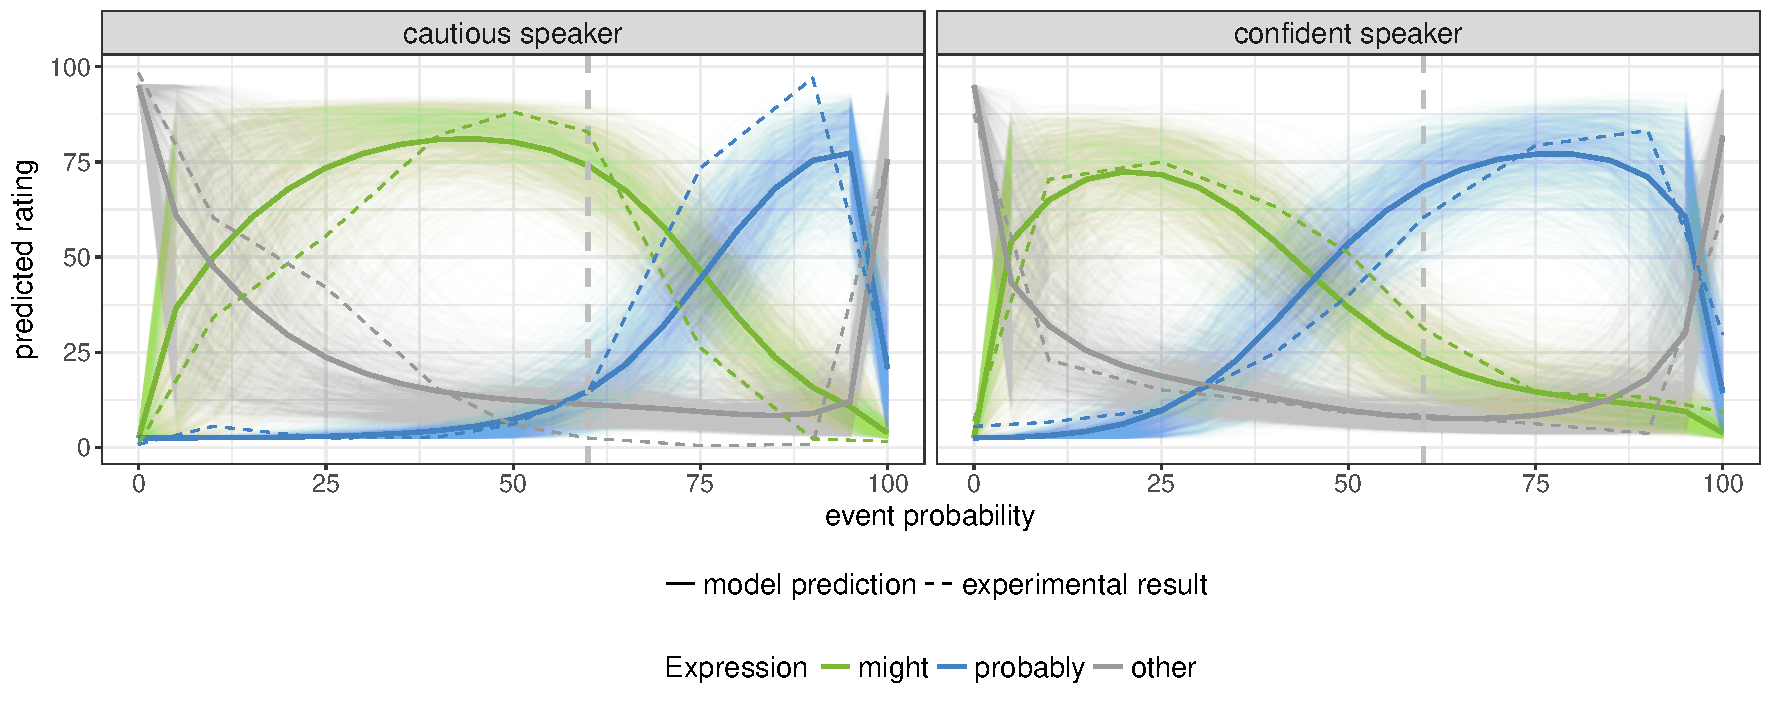
\includegraphics[width=\textwidth]{plots/adaptation-posterior-predictions-replication.pdf}
  \caption{Post-adaptation model predictions from simulations for Experiment~2 and experimental results. 
  The solid lines shows the mean model predictions and the thin lines around the mean show the distribution of model predictions. \label{fig:post-exposure-model}}
\end{figure}

Apart from quantitatively assessing the fit of the model, it is informative to visually inspect the predictions of the model to verify that the model makes correct qualitative predictions. 
Figure~\ref{fig:post-exposure-model} shows the post-exposure predictions of the \textit{cost \& threshold distributions} model compared to the average participant ratings for the two conditions from Experiment~2.
%\footnote{
%We only discuss the simulations for Experiment~2a in this section. See Appendix~E for the same plots for the simulations for Experiment~2b.} 
Qualitatively, 
the model captures several important patterns in the post-adaptation behavior. The model correctly predicts that in the \textit{cautious speaker} condition, ratings for \textsc{might} are 
higher than ratings for \textsc{probably} when there is an objective probability of 0.6. For the \textit{confident speaker} condition, the model correctly predicts the
opposite pattern. The model also predicts that in the \textit{cautious speaker} condition, participants rate \textsc{might} highly for a larger range of event probabilities than
in the \textit{confident speaker} condition and the model predicts the  reverse pattern for the \textsc{probably} ratings. Further, the model predicts that high ratings for \textsc{might} 
and \textsc{probably} are not limited to the utterance-event probability combinations that participants observed during the exposure phase. For example, the model correctly predicts
high ratings of \textsc{might} for low event probabilities in the \textit{cautious speaker} condition despite the fact that it never observed utterances for low event probabilities. Similarly,
the model predicts high rating of \textsc{probably} for high event probabilities in the \textit{confident speaker} condition -- a combination which was again not part of the exposure trials
of this condition.

Quantitatively, there are some differences between the model predictions and participant behavior. This is not surprising considering that the model predictions are a result of simulations
and, with the exception of the three variance parameters of the prior distributions, we did not fit any model parameters to the behavioral data. One difference is that the model underpredicts 
the ratings of one of the  \textsc{probably} utterances in the \textit{cautious speaker} condition.
 One reason for this deviation could be the relatively simple prior structure. For the priors, we made the assumption that all model parameters are independent of each other and 
that the variance for the different parameter types is the same for all utterances. However, it could be that listeners have more structured prior beliefs such that priors over different parameters are correlated or
variances of prior distributions differ. For example, it could be that listeners expect the thresholds for \textit{might} and \textit{probably} to be correlated such that higher thresholds for \textit{might} are correlated 
with higher thresholds for \textit{probably}. Or it could be that listeners expect more between-speaker variation for some expressions than for others. Considering that we only have data from two experiments to test
model predictions and therefore would likely overfit to the data if we tried to fit more complex prior structures with more parameters, we leave the investigation of the exact structure of listeners' prior beliefs to future work.

\begin{figure}
  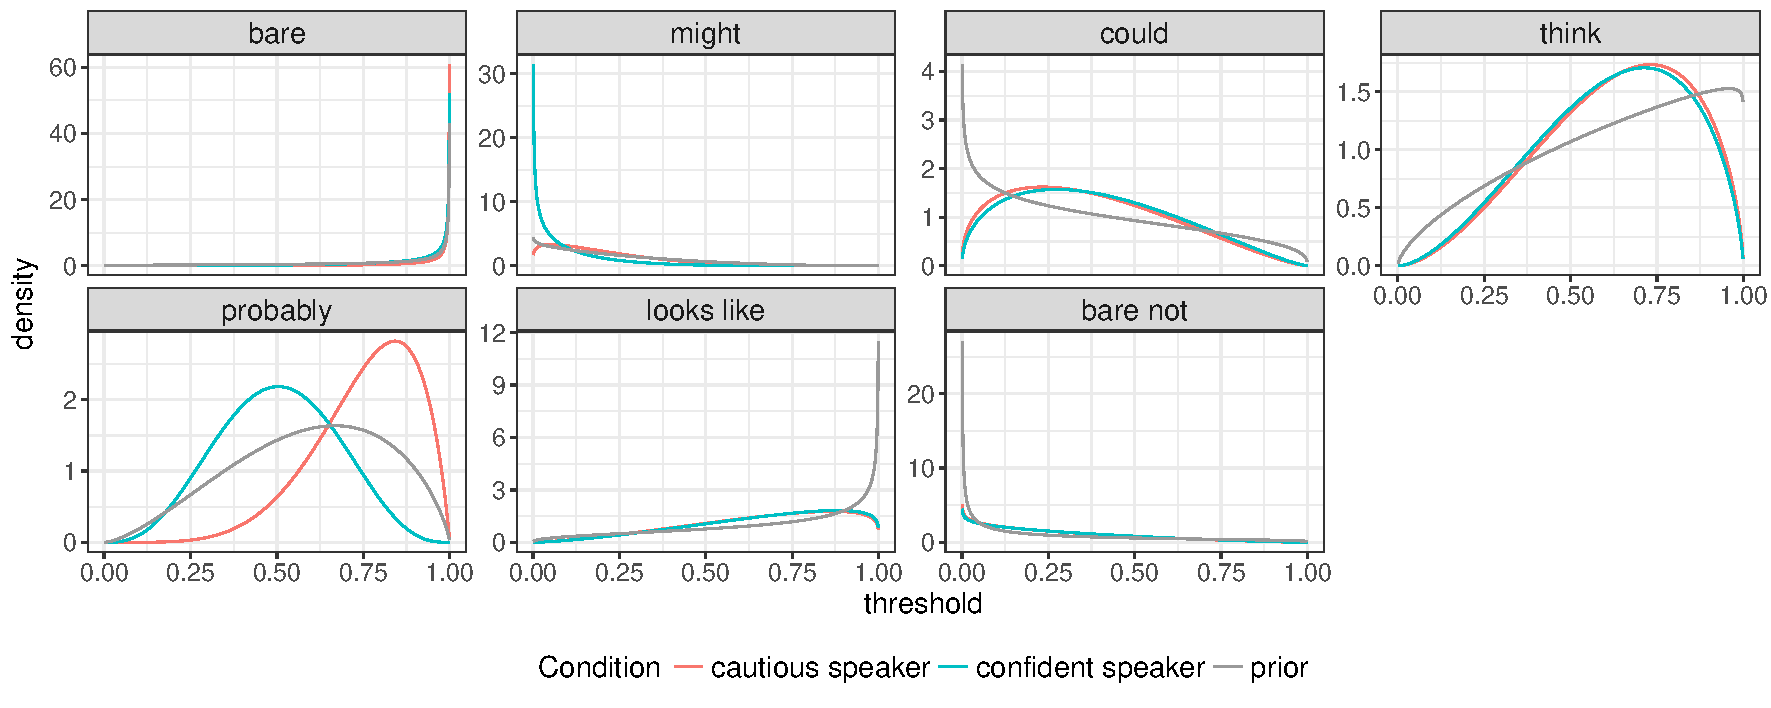
\includegraphics[width=\textwidth]{plots/adaptation-posterior-thresholds-replication.pdf}
  \caption{Post-adaptation threshold distributions from the simulations for Experiment~2. \label{fig:post-exposure-thresholds}}
\end{figure}




The second noticeable deviation is that in the \textit{confident speaker} condition, the model overpredicts the ratings of the \textsc{other} utterance for event probabilities of 1 . This prediction is primarily driven by high values for the predicted ratings of \textsc{bare}. However, we argue that the model predictions in this case are reasonable, and that the lower participant ratings are likely an artifact of the experimental task. After completing the experiment, 
several participants indicated in a feedback form that they were confused by the lack of an option to rate the \textsc{bare} utterance, 
which they had heard during the exposure phase. In light of this confusion, almost all individual participants chose among two strategies when there was an event probability of 1: they either provided a rating of 100 for \textsc{other} 
or they provided a rating of 100 for \textsc{probably}, which on average leads to the ratings shown in \figref{fig:post-exposure-model}.

With the exception of these two deviations, the model makes not only correct qualitative, but also accurate quantitative predictions for the post-exposure ratings.

Lastly, we can also inspect how the model arrived at its predictions by looking at the inferred model parameters.  
Figures~\ref{fig:post-exposure-thresholds} and \ref{fig:post-exposure-costs} show the inferred
post-exposure threshold distributions and costs for the two conditions as well as the distributions inferred from the norming data.
Figure~\ref{fig:post-exposure-thresholds} shows that the threshold distribution for \textit{probably}
changed considerably depending on the exposure phase: in the \textit{cautious speaker} condition,
its mean shifted to a higher value than  inferred from the norming data; in the \textit{confident speaker} condition the mean 
shifted to a lower value. To a lesser extent, we observe similar shifts in the mean of the threshold
distributions for \textit{might}. We further observe that for all expressions, the variance of the threshold
distributions decreased as a result of adaptation. In the case of the expressions that were part of the exposure
phase, this is expected, since the exposure speaker used these expressions very consistently; in the case of the
other expressions, this decrease in variance is a result of the exponential prior over the population parameter,
which biased the model towards lower variance. For some of the thresholds, this resulted in differently shaped distributions.
However, note that the area under the curve of all threshold distributions except for \textit{probably} is still very similar to the 
area under the curve of the norming data threshold distributions. And overall, except for the distributions
for \textit{might} and \textit{probably}, the post-exposure threshold distributions are almost identical in both conditions.
This suggests that the post-adaptation expectations 
are in part a result of updated threshold distributions for \textit{might} and \textit{probably}.

\begin{figure}
\center
  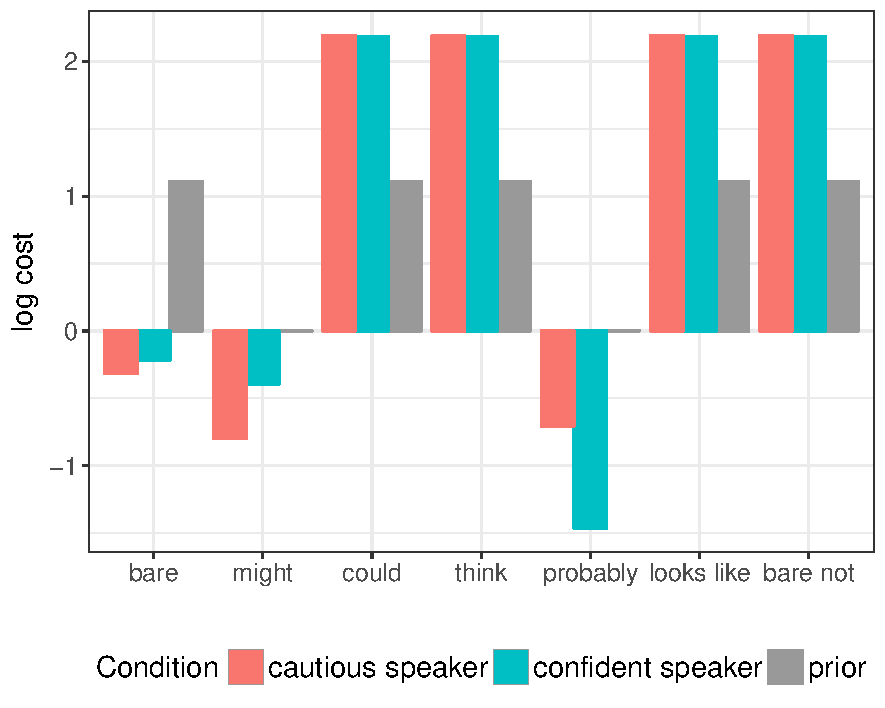
\includegraphics[width=0.5\textwidth]{plots/adaptation-posterior-costs-replication.pdf}
  \caption{Post-adaptation $log$ cost values from simulations for Experiment~2. Note that the cost of \textsc{might} and \textsc{probably} 
  in the norming data model was 1 and therefore the $log$ cost for these utterances is 0. \label{fig:post-exposure-costs}}
\end{figure}

Figure~\ref{fig:post-exposure-costs} shows that the costs of the \textsc{might}, \textsc{probably} and
\textsc{bare} utterances, i.e., the three utterances that participants observed during the exposure phase,
all decreased while the costs of the other four utterances increased compared to the costs inferred from the norming
data. Further, the post-exposure cost of \textit{might} is lower than the cost of \textit{probably} in the \textit{cautious speaker} condition
and the opposite relation between these costs holds in the \textit{confident speaker} condition, which suggests that
that the post-adaptation expectations are in part also a result of updated beliefs about preferences of \textsc{might} and \textsc{probably}. 
\add{This finding also highlights the complex interplay between threshold distributions and preferences: The number of exposure trials 
with \textsc{might} and \textsc{probably} was identical in both conditions, so participants could not have inferred a preference
based on exposure frequencies. Instead, participants seemed to indirectly infer that the \textit{cautious speaker} prefers to use \textsc{might} from the speaker's uses of \textsc{might} to describe a
larger range of event probabilities and that the \textit{confident speaker} prefers to use \textsc{probably} from the speaker's uses of \textsc{probably} for a
larger range of event probabilities. However, frequency nevertheless has an effect on inferred preferences. As shown in Appendix~F, the difference in inferred preferences 
was larger when participants in the \textit{cautious speaker} condition were exposed to more trials with \textsc{might} than in the \textit{confident speaker} condition and participants in the \textit{confident speaker} condition were exposed to more trials with \textsc{probably} than in the \textit{cautious speaker} condition.}


% These cost differences
%are expected considering that the number of exposure trials across the two conditions differed (in the \textit{cautious speaker} condition in Experiment~2a there were more trials
%with \textsc{might}; in \textit{confident speaker} condition more trials with \textsc{probably}). More surprisingly, this pattern
%persisted in the simulations for Experiment~2b in which the exposures of these two utterances were balanced across conditions 
%(see Appendix~E for cost plot for balanced simulations).
%These persistent differences suggest that the post-adaptation expectations 
%are in part also a result of updated beliefs about preferences of \textsc{might} and \textsc{probably}. 

%Further, the observation that this difference persisted even if the frequency of exposure utterances
%was matched across conditions, provides some evidence that uncertainty expression preferences
%are not only determined by observed utterance frequencies but instead are also influenced 
%by the contexts in which the the expressions are used. 
%

\subsection{Interim summary}

In the previous two sections, we presented the results from an experiment that provides strong evidence for
listeners updating expectations about a speaker's use of uncertainty expressions after brief
exposure to that speaker. We further presented a computational adaptation model which models the adaptation
process as an instance of Bayesian belief updating. Using different implementations
of that model to investigate which kind of expectations listeners update during adaptation, we found strong evidence that listeners update beliefs both about  threshold distributions and 
 about speaker preferences.

\section{Experiment 3: Effect of adaptation on interpretation}
\label{sec:exp-model-interpretation}


Up to this point, we focused on listeners' expectations about a speaker's use of uncertainty expressions. As we discussed
in the introduction, we expect updated expectations to also have an effect on the \emph{interpretation} of uncertainty expressions. This
effect is also predicted by RSA models,  which assume that a pragmatic listener $L_1$ tries to infer the state of the world (in our case, the event probability $\phi$) by reasoning
about their prior beliefs about the world state and their expectations about a speaker's language use (in our case, the expected pragmatic speaker $ES_{1}$) via Bayes' rule:

$$ L_1(\phi \mid u_e) \propto P(\phi) ES_1(u_e \mid \phi).$$

According to such a model of interpretation, the shifts in expectations that we observed in the previous experiment should also lead to a shift in interpretations. 
If we assume a uniform prior over event probabilities,\footnote{To reiterate, this assumption was motivated by the study reported in Footnote 9, which suggested that participants on average assign equal probability to each gumball machine a priori. In this special case, we expect interpretations to be an exact mirror image of production expectations but in many other scenarios, listeners will have skewed prior beliefs about the event likelihood (e.g., consider beliefs about the likelihood of rain on a specific summer day in California, which will be highly skewed towards low values) and in such scenarios, listeners integrate prior beliefs and  production expectations to arrive at interpretations.} then the model predicts that listeners who were exposed to a \textit{cautious} speaker should infer 
higher event probabilities when hearing {\sc might} or {\sc probably} than listeners who were exposed to a \textit{confident} speaker. Figure~\ref{fig:post-exposure-comp}
shows the distribution over event probabilities after hearing three different utterances as predicted by $L_1$ parameterized by the inferred parameters from our
adaptation simulations in the previous section. As these plots show, in the \textit{cautious speaker} condition, the distribution over event probabilities after hearing \textit{might} 
and \textit{probably} is shifted towards higher values as compared to the distributions in the \textit{confident speaker} condition. 

\begin{figure}
  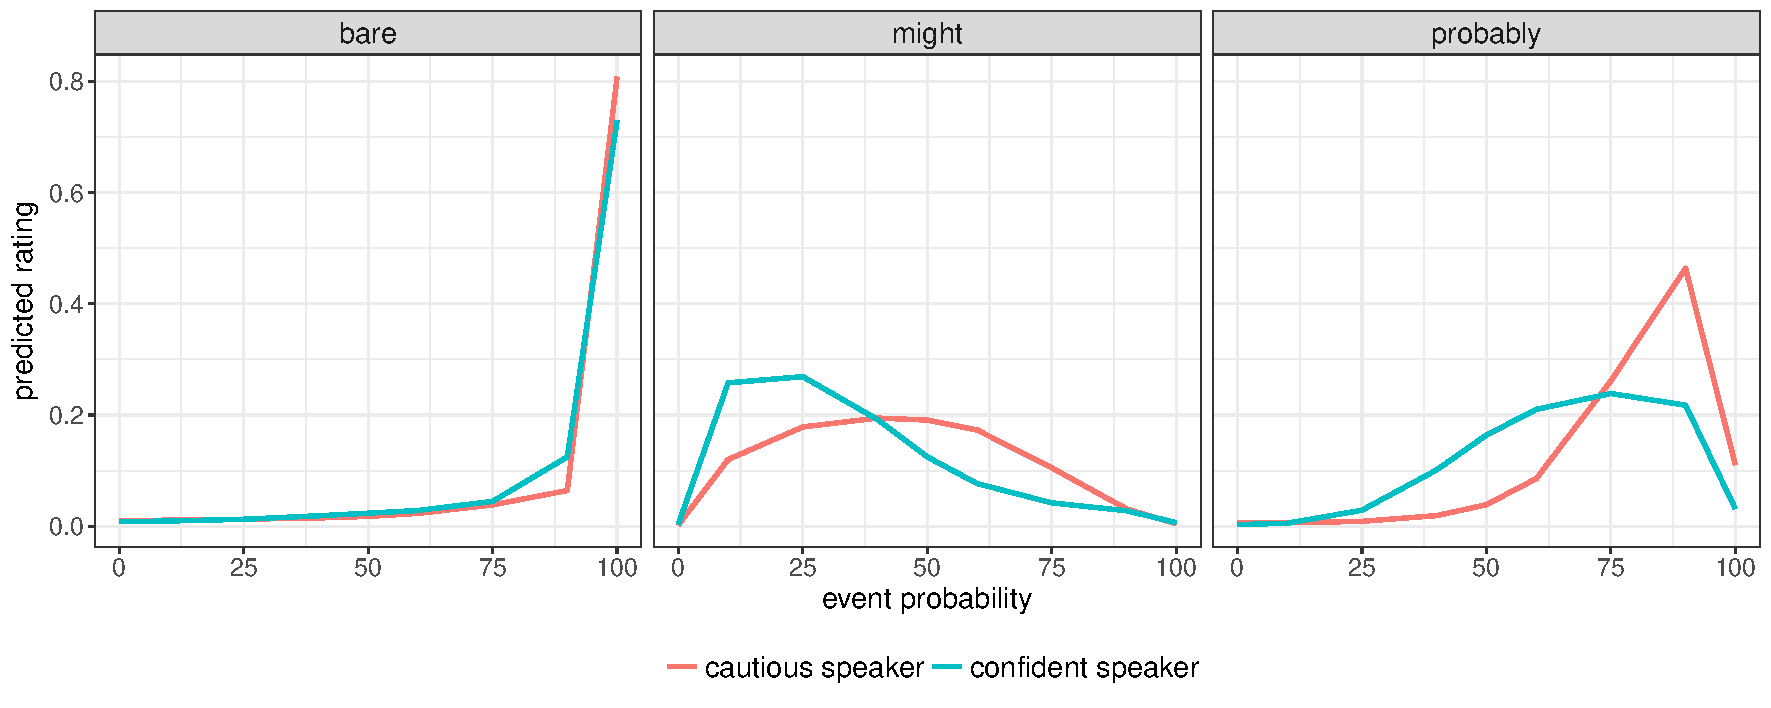
\includegraphics[width=\textwidth]{plots/adaptation-posterior-comp.pdf}
  \caption{Post-adaptation interpretation distributions for the utterances  \textsc{bare}, \textsc{might}, and \textsc{probably} as predicted by the pragmatic listener $L$\textsubscript{$1$}. \label{fig:post-exposure-comp}}
\end{figure}

In this experiment, we tested whether this prediction is correct and whether listeners' change in expectations transfers to a change in interpretations. 
The procedure, materials and analyses were pre-registered at \url{https://osf.io/ghnc3}.\footnote{This experiment is a modified version of a previous experiment, which qualitatively yielded the same results but seemed to confuse some participants. See Appendix~G for a discussion of the original experiment.}

\subsection{Method}

\subsubsection{Participants}

We recruited a total of 80 participants (40 per condition) on Amazon Mechanical Turk. We required participants to have a US-based IP address and a minimal approval rating of 95\%. Participants were paid \$1.5 which amounted to an hourly wage of approximately \$15. None of the participants had participated in any of the previous experiments. 

\subsubsection{Materials and Procedure}

Participants completed a set of exposure trials followed by a set of test trials. The exposure trials were identical to the exposure trials in Experiment~2. The test trials probed participants' interpretations of the utterances {\sc might}, {\sc probably} and {\sc bare}. On each test trial, participants listened to a recording of the speaker from the exposure phase producing {\sc might}, {\sc probably} and {\sc bare} and then participants were asked to rate for 9 gumball machines with the same proportions of blue and orange gumballs as in the previous experiments how likely they thought it was that the speaker saw each of these gumball machines by distributing coins.  Participants distributed 10 coins per trial and completed 6 trials in total  -- one for each expression-color pair. The exposure phase again contained  6 attention check as in the previous experiment. However, given the low attention check performance in the previous experiments, we modified the attention checks. Instead of asking participants whether they saw an X on the previous trial, we asked participants to choose the gumball machine that they had seen on the previous trial among two machines displayed in random order.

\subsubsection{Exclusions}

We excluded participants who failed more than 2 attention checks, which led to 1 exclusion in the \emph{cautious speaker} condition and 1 exclusion in the \emph{confident speaker} condition.


\subsubsection{Analysis and Predictions}

If participants update their expectations of a specific speaker's use of uncertainty expressions,  we expect them to interpret a more confident speaker's utterance 
to communicate a lower event probability than a more cautious speaker's utterance. We tested this prediction by treating participant's distributions of coins 
of gumball machines as a probability distribution over gumball proportions (and consequently event probabilities).  For each utterance, we 
normalized participants' coin distributions such that they summed up to 1, so that we could interpret the normalized scores 
as a categorical probability distribution over gumball machines given an utterance. We then compared the resulting distributions
over target color gumball proportions for each utterance in terms of their expected value, using a $t$-test.
 We predicted that the expected values of 
{\sc might} and {\sc probably} would be larger in the \emph{cautious speaker} condition than in the \emph{confident speaker} condition.

\subsection{Results and Discussion}

\begin{figure}
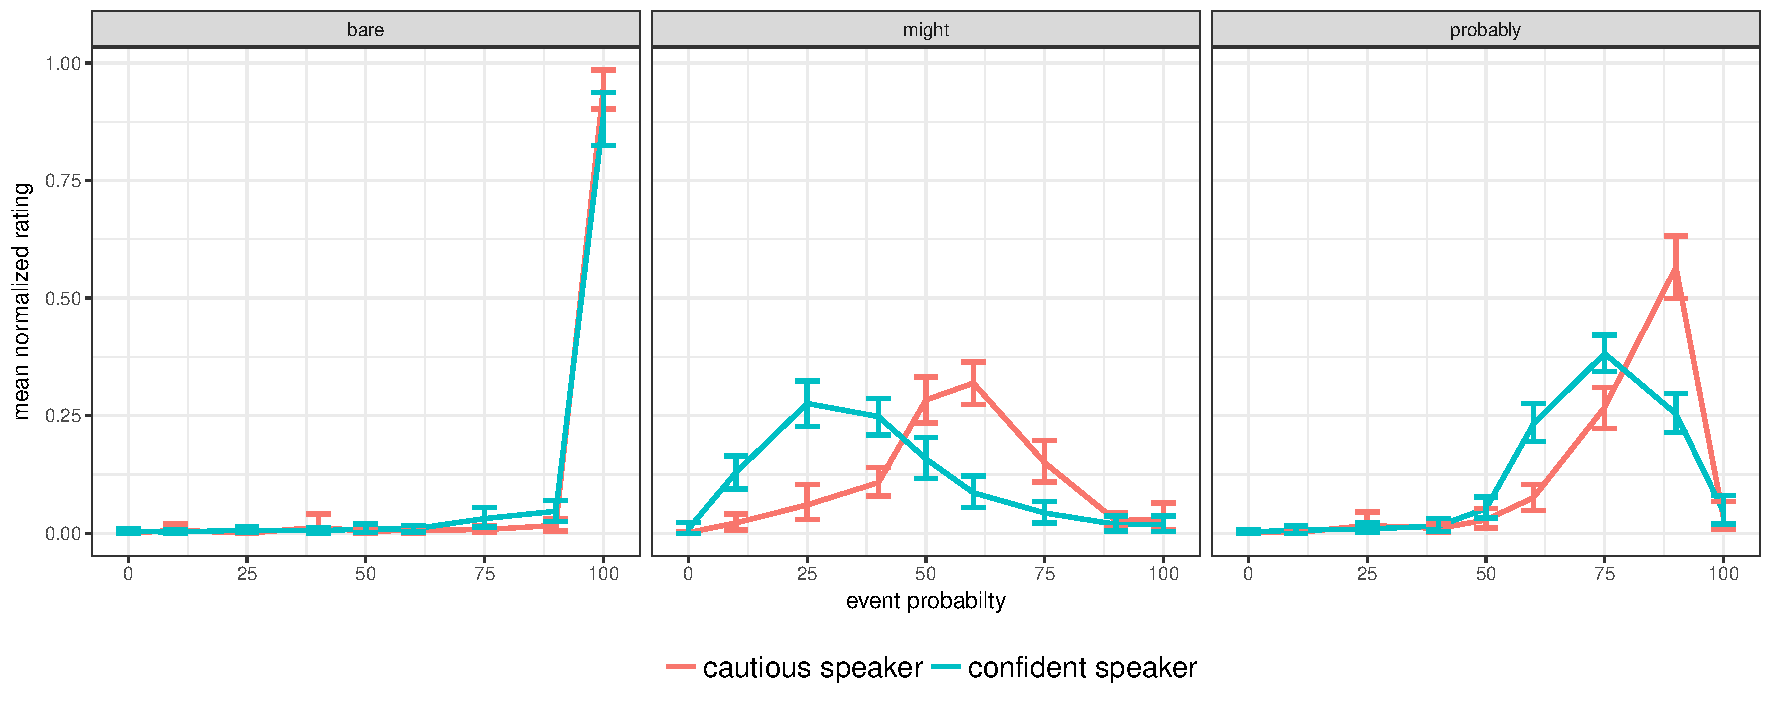
\includegraphics[width=\textwidth]{plots/exp-2-ratings.pdf}
\caption{Aggregated post-exposure ratings from Experiment~3. Error bars correspond to bootstrapped 95\%-confidence intervals.  \label{fig:adaptation-results-comp}}
\end{figure}

Figure~\ref{fig:adaptation-results-comp} shows the aggregated and normalized ratings for the two conditions.  As predicted, participants provided higher ratings for gumball machines with higher target color percentages after hearing {\sc might} and {\sc probably} in the \emph{cautious speaker} condition than in the \emph{confident speaker} condition. This also led to a significantly higher expected value for {\sc might} ($t(76)=5.84$, $p<0.001$) and {\sc probably} ($t(76)=3.92$, $p<0.001$) in the \emph{cautious speaker} condition as compared to the \emph{confident speaker} condition.

These results suggest that listeners not only update their expectations about a speaker's use of uncertainty expressions, but also use those updated expectations in interpretation. 
Here, we made the implicit linking assumption that the distribution of coins reflects participants'  beliefs about event likelihoods after hearing an utterance.
The choice for this paradigm, which is very similar to betting paradigms that have been used to study utterance interpretation in reference games \parencite{Frank2012,Goodman2013} as well as for probing subjective probabilities \parencite[e.g.,][]{Hampton1973}, was motivated by the assumption that listeners will have uncertainty about the exact event likelihood after hearing \textsc{might} or \textsc{probably}. Allowing
participants to assign multiple coins to gumball machines with different proportions provided them with the ability to convey this uncertainty. The results from this experiment suggest that
participants behaved as expected: they assigned almost all coins to the gumball machine with 100\% target color gumballs after hearing \textsc{bare}, 
an utterance about whose interpretation participants likely have very little uncertainty, whereas they assigned coins to multiple machines after hearing \textsc{might} or \textsc{probably}. 


\subsection{Model comparison}

\begin{table}
\center
\begin{tabular}{r | c | c }
Model &   odds & $R^2$   \\ \midrule
fixed  & $10^{-452}$ & 0.827     \\
cost  &  $10^{-231}$ & 0.883       \\
threshold distributions  & $10^{-129}$ & 0.887 \\
cost \& threshold distributions & 1 &   0.936     \\
\end{tabular}
\caption{Model evaluation results on data from Experiment~3.  \textit{odds} are the posterior likelihood odds of the models compared to the \textit{cost and threshold distributions} model. $R$\textsuperscript{$2$} are computed between  the mean post-exposure ratings and the mean model predictions.  \label{tbl:model-comparison-comp}}
\end{table}



We return again to our main research question regarding which expectations are updated during adaptation. The production expectation experiments and model simulations provided strong evidence for listeners updating 
their beliefs about the threshold distributions and preferences. 
To determine the stability of these results, we also compared the pragmatic listener $L_1$ predictions from the simulations with different prior structures to the post-exposure ratings in Experiment~3. To this end, we computed the predictions of the $L_1$ model from the
posterior distributions over model parameters that we obtained through the simulations in the previous section. \tableref{tbl:model-comparison-comp} shows the model fit
for the different types of simulations. As this table shows, the model according to which both threshold distributions and costs are updated provides the best fit according to both metrics. 
Considering that the posterior likelihood odds consistently favored this model in all model comparisons, we take these results together as strong evidence that listeners update their expectations about threshold distributions
and costs. 

\subsection{Model evaluation}


\figref{fig:post-exposure-comp-data} superimposes the model predictions and the experimental data. As these plots show, the model accurately captures most of the qualitative and quantitative patterns. First, 
the model makes both qualitatively and quantitatively accurate predictions for the interpretation of the \textsc{bare} utterance in both conditions. Second, the model makes the crucial qualitative prediction that participants expect the speaker to communicate lower event probabilities in the \textit{confident speaker} condition than in the \textit{cautious speaker} condition, which we also observed in Experiment~3. Further, even though we used the parameters that we obtained in the simulations from the previous section and did not fit any parameters to the data from Experiment~3, the model also provides good quantitative predictions of participant's interpretation of \textsc{might} and \textsc{probably},
which provides further support for the hypothesis that semantic/pragmatic adaptation is an instance of Bayesian belief updating.

The main deviation between the model predictions and the experimental data lies in the interpretation of \textsc{might} in the \textit{cautious speaker} condition. For this interpretation, the model predicts a less peaked distribution than the empirical distribution.  One explanation for this deviation could be that participants are considering alternative uncertainty expressions (e.g., \textit{very unlikely}) that we did not include in the model.  However, since fine-tuning the set of alternative utterances would not change the qualitative predictions of the model and would not provide additional theoretical insights, we leave a more detailed exploration of this issue to future work. 

\begin{figure}
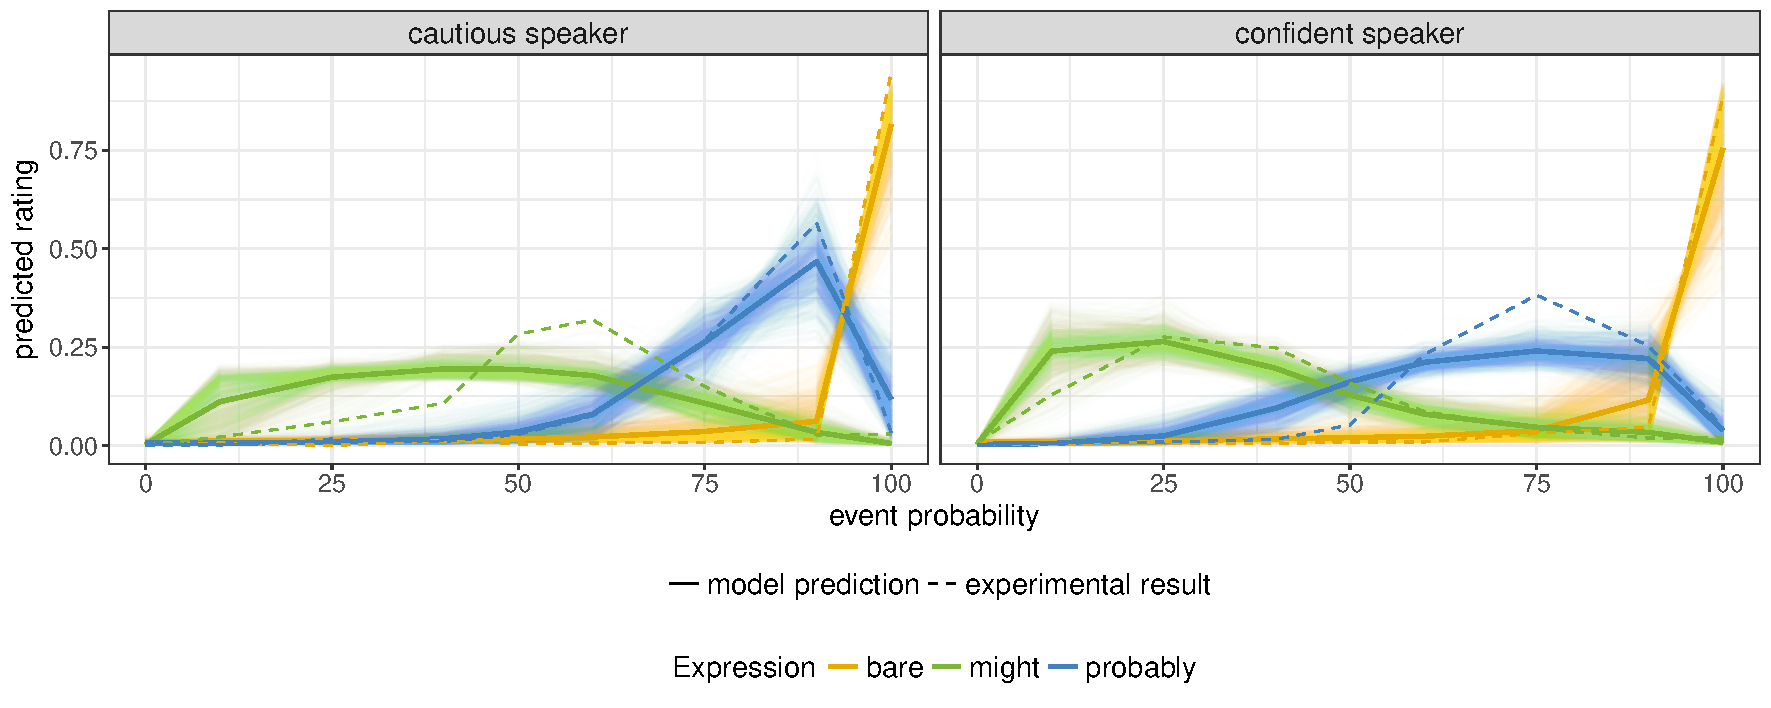
\includegraphics[width=\textwidth]{plots/adaptation-posterior-comp-data.pdf}
\caption{Predictions of \textit{threshold distributions and costs} model and data from Experiment~3. The thin lines around the mean show the distribution of model predictions.  \label{fig:post-exposure-comp-data}}
\end{figure}

\section{General Discussion}

While adaptation in language is a widely attested phenomenon, the nature of the representations that are updated during semantic/pragmatic adaptation has largely remained a mystery. In this paper our contribution has been three-fold: %first, we identified a novel domain in which semantic/pragmatic adaptation occurs, that of uncertainty expressions;  second, we investigated the nature of the representations that are updated during adaptation via the comparison of computational models of adaptation formulated within a Bayesian pragmatic modeling framework; and third, we tested a novel prediction resulting from the application of this model to interpretation.  

%\jd{i commented this first paragraph back in with minor changes because i do think it's worth reminding people of the point of doing all this work!}

First, in a production expectation experiment (Experiment~2), we showed that listeners adapt to speakers who vary in their use of uncertainty expressions, demonstrating that that 
the findings from \textcite{Yildirim2016} extend to the class of uncertainty expressions. Second, we showed that updated \emph{production} expectations also affect subsequent utterance \emph{interpretation}  (Experiment~3). Finally, in a series of model comparisons, we found strong evidence for listeners updating their beliefs about both the speaker's lexicon as well as the speaker's preferences, which suggests
that semantic/pragmatic adaptation is a result of updating both of these representations. We further found that modeling the adaptation process as an instance of Bayesian
belief updating explains participants' post-adaptation behavior in both the production expectation (Experiments~2) and comprehension (Experiment~3) experiments. 


We next discuss the implications of this work for other accounts of adaptation and for semantic theories of uncertainty expressions, as well as its methodological implications. We then turn to limitations of the current results and account and discuss promising future research avenues this work opens. 



\subsection{Implications for and relation to other accounts of adaptation}

The model in this paper is formulated at the computational level \parencite{Marr1982,Anderson1990} 
and is therefore directly only comparable to other computational models. However, we can still assess 
the compatibility of our findings with mechanistic accounts. We first discuss the relation to existing computational 
models of adaptation and then discuss what the results tell us about existing mechanistic accounts of
 adaptation.

The model presented above follows several other computational models of linguistic adaptation that are based 
on Bayesian belief updating, including models of phonetic adaptation \parencite{Kleinschmidt2015}, syntactic 
adaptation \parencite{Kleinschmidt2012}, adaptation in the interpretation of prosodic cues \parencite{Roettger2019},
and adaptation to variable use of the quantifiers \textit{some} and \textit{many} \parencite{Qing2014}. 
All of these models are based on the same Bayesian belief updating procedure according to which listeners integrate
their prior linguistic expectations and observed linguistic behavior to form updated expectations that facilitate comprehension.
This updating procedure is in line with recent proposals of a ``Bayesian brain'' \parencite[e.g.,][]{Clark2013,Friston2010} which argue that
many cognitive and perceptual processes can be seen as an instance of integrating prior beliefs with observed signals from the environment.

%TODO: is there something we can say about a shared cognitive process?
%Considering that these models that are all based on the same belief updating procedures can explain adaptation behavior 
%from a range of linguistic domains, it is possible that linguistic adaptation is a result of cognitive processes that operate in 
%a similar fashion at all levels of linguistic representation. 

Similarly, the formation of conceptual pacts \parencite{Clark1986} --  alignment in the formation of referring expressions -- has been explained using a model  similar to the one we have proposed here \parencite{Hawkins2017}. Hawkins et al.'s model is based on the assumption that speakers and listeners have uncertainty about the lexicon \parencite[see also][]{Bergen2016} and that in interaction, speakers 
and listeners update their beliefs about the shared lexicon, akin to the updating of threshold distributions 
in our model. This further suggests that belief updating plays an important role in partner-specific language processing.


In the space of mechanistic accounts, \textcite{Pickering2004} argued that a lot of partner-specific linguistic behavior
 can be explained as the result of priming, i.e., the automatic activation of linguistic representations when 
a speaker produces an utterance or a listener hears an utterance. Their account has the appeal
of explaining why partner-specific language use often appears to happen automatically and effortlessly. 
With the additional stipulation that the activated representations include information about both language
and the situational context and thus are able to represent variable semantics of uncertainty expressions,
their account appears to be compatible with our results. However, considering that \textcite{Yildirim2016} and 
\textcite{Schuster2019} found that listeners form speaker-specific expectations rather than expecting speakers
to behave like the most recent speaker they encountered, adaptation seems to be a more complex process than predicted by a
priming account.

In a more recent proposal, \textcite{Pickering2013} agued that
at least sometimes listeners perform \textit{prediction-by-association} when processing
an utterance, that is, listeners make predictions about what the speaker would say based on
the context and their experience with the speaker.  This appears to
be compatible with our computational adaptation model but more details need to be
worked out about how such predictions operate at the implementational level \parencite{Marr1982}.

In a second line of work, \textcite{Horton2005,Horton2016} argued that partner-specific
language use can be explained by an episodic memory account \parencite{Goldinger1998,Johnson1997,Pierrehumbert2001}.
According to this account, individual linguistic events are encoded together with
speaker information and the world state in memory, which results in speaker-specific
linguistic representations. This account is compatible with our findings, if we assume
that individual utterance-world state pairs are stored in memory together with the speaker's 
identity, and that some additional inference mechanism gives rise to the more complex
pragmatic behavior that we observed in our experiments.

% -- question about associative memory vs. error correction (still unclear) (look again at Brown-schmidt 2016)


\subsection{Implications for the semantics of uncertainty expressions}

Our results also have implications for semantic theories of uncertainty expressions.
The finding that listeners rapidly update their beliefs about semantic thresholds of uncertainty expressions
suggests that the semantics of these expressions is highly dynamic and context-sensitive. This is broadly compatible with 
theoretical accounts of probability operators \parencite[a subset of uncertainty expressions; e.g.,][]{Yalcin2010} which 
state that the meanings of probability operators are highly dynamic and largely determined by the context. Our results
suggest that the meaning of uncertainty expressions is even more dynamic than predicted by these accounts. First, we show that this dynamicity 
extends to a broader set of uncertainty expressions than is typically considered (e.g., \textit{might}), as has been recently also argued by \textcite{Lassiter2016}. 
Second, while these accounts generally assume 
that the main source of variability in interpretation is the probability of the event
embedded under the uncertainty expressions, we find that knowledge of speaker identity also  importantly contributes variability.

Dynamic and context-sensitive semantics have also been proposed for many other types of expressions.
For example, \textcite{Clark1983} argued that speakers and listeners
are able to compute novel senses of nouns and verbs on the fly. Similarly, in the domain of gradable adjectives such as \textit{tall},
 \textcite{Kennedy2007} and many others have argued that the interpretation of these adjectives crucially depends on contextual
 parameters. Considering the prevalence of dynamic meanings for so many other types of expression, it is therefore not 
 surprising that the interpretation of uncertainty expressions also appears to be highly context-sensitive.
 
\subsection{Methodological implications}

Our results also have implications for conducting psycholinguistic experiments. First,
the finding that listeners adapt to the statistics of their environment within a short experiment
suggests that experimenters should be cognizant of potential adaptation effects when probing
production expectations or interpretations of uncertainty expressions \parencite[see also][]{Jaeger2010}. 

Further, the results of Experiment~1, and in particular, the finding
that participants' expectations about the use of utterances in the experiment strongly depended on
the alternative utterances that we provided, highlights the need to be cautious about drawing general conclusions about expectations of use from single experiments. For example,
had we only considered the results from the \textit{bare-might} condition (see \figref{fig:norming-results-main}),
we might have concluded that ``might'' is an expected expression to communicate an event probability of 75\%,
whereas if we had only considered the results from the \textit{might-probably} condition we might have instead concluded that it is \emph{not} an expected expression to communicate an event probability of 75\%.
This is where explicit modeling of the sort we have engaged in here is hugely helpful: formulating a concrete linking function which models the effects of 
alternatives allows for inferring the latent meanings of utterances by combining data from different experiments \parencite[see also][for similar approaches]{Franke2014,Peloquin2016}.

\subsection{Limitations and future directions}

One limitation of the present research is that the experimental paradigm is not interactive and that participants likely engaged in meta-linguistic reasoning in providing production expectation and interpretation ratings. While we tried to make the communicative situation depicted in the experiments natural,
the paradigm is clearly different from everyday dialog. This limitation was necessary for the tight coupling between the experimental work
and the model simulations that allowed us to investigate what kind of representations listeners update during adaption; in a more
naturalistic and unconstrained setting, we would not have been able to obtain information about listener's production expectations and about their
uncertainty in both production expectations and interpretations. However, considering that our task was different from everyday interactions, investigating
to what extent the results in the present research translate to less scripted and more interactive settings is an important area for future research. Employing measures like eye movements or mouse-tracking could provide insight into whether participants' updated beliefs affect online language processing, i.e.~where meta-linguistic reasoning is unlikely to occur. In this vein, mouse-tracking has recently been
employed  to investigate the incremental nature of adaptation in the domain of  prosodic cues \parencite{Roettger2019}. Both eye-tracking and mouse-tracking experiments 
allow for implementing more natural interpretation tasks while still providing information about participants' uncertain beliefs via fixation patterns or cursor trajectories.


Throughout this paper, we made the assumption that listeners  form \textit{speaker-specific} production expectations. However,
since all our experiments had a between-subjects design, it could be that participants were only adapting to the experimental
situation, independent of the speaker. This seems unlikely given the results reported by \textcite{Yildirim2016}, who found that
participants formed speaker-specific production expectations after being exposed to multiple speakers whose use of
quantifiers differed. Moreover,  \textcite{Schuster2019} have provided evidence of speaker-specific adaptation to 
uncertainty expressions. However, exactly which aspects of a situation (e.g., the speaker, the topic of conversation, the visual context, etc.)
listeners adapt to is an issue that merits further investigation.

%\jd{i commented out the WEIRD and cross-linguistic issue because this doesn't seem sth that's specific enough to just this phenomenon}
%Further, we investigated adaptation to uncertainty expressions only for English 
%and all our participants were from the US. Our model does not make any
%assumptions specific to English, so we expect that similar adaptation behavior could
%be observed with speakers of other languages but another interesting avenue for future
%research would be to investigate adaptation behavior for languages other than English, in
%particular in non-WEIRD societies.

One advantage of formalizing a theory as a computational model is that the model 
makes concrete predictions to test in future experiments. For example, the proposed
model is able to make quantitative predictions about the relation between the number of exposure
trials and the size of the adaptation effect. Qualitatively, the model predicts that more exposure
should lead to more adaptation, for which some evidence is reported by \textcite{Schuster2019}.
However,  a systematic investigation of whether the model makes the correct quantitative predictions remains to be conducted. 

%priors and acquisition

Further, the presented adaptation model is built around the assumption that the utility of an utterance is exclusively determined
by the informativeness and the cost of the utterance. However, it has been observed that other speaker goals such as being polite or
convincing could also factor into the interpretation of uncertainty expressions \parencite[see e.g,][]{Pighin2011,Juanchich2013,Holtgraves2016}.
It could therefore be that, for example, listeners explain away the behavior of a ``confident'' speaker if the context suggests that the speaker
has an incentive to be encouraging or has additional goals besides being informative \parencite[see also][]{Yoon2016,Yoon2017}. Investigating whether listeners draw such complex inferences
could provide  insight about which kind of potential speaker goals enter into listeners' pragmatic reasoning process.


\subsection{Conclusion}

We began with the puzzle of how to reconcile the assumption of stable utterance alternatives required for pragmatic reasoning with variability in speakers'  language use. The work reported here, building on much previous work on adaptation, suggests that this apparent tension is easily resolved if listeners form speaker-specific utterance expectations that they can recruit when interpreting utterances produced by that speaker.

In a series of web-based experiments, we found that after exposure to a specific speaker, listeners rapidly update 
their expectations about which uncertainty expressions that speaker is likely to produce
to describe varying event probabilities. Moreover, these updated expectations also enter into subsequent utterance interpretation.
We provided a formal account of semantic/pragmatic adaptation and modeled this behavior using a Bayesian cognitive model 
which assumes that (listeners reason about) speakers (who) efficiently trade off utterance informativeness and cost.
Through a series of simulations we found strong evidence that semantic/pragmatic adaptation is the result of
updating beliefs about both a specific speaker's underlying lexicon as well as the speaker's utterance
preferences. These results both provide new insights into the cognitive processes involved in semantic/pragmatic adaptation
and demonstrate that tight coupling of quantitative computational models and experimental results can shed light on
unobservable representations.

\printbibliography


\appendix
\renewcommand{\thesection}{\Alph{section}}

\section{Effect of color in Experiment~1}
\setcounter{section}{1}


As mentioned in a footnote, we ran the norming studies in three batches using three slightly different procedures across conditions. We originally ran condition 0 (\emph{bare-might}) as a pilot condition. In the results, we noted that participants did not differ in their ratings depending on whether the girl asked for a blue or an orange gumball ($R^2(27)=0.997$ between mean ratings for blue and orange trials). To lower the number of trials, we therefore asked each participant to provide ratings for only one of the two colors (randomized across participants) for the next batch of conditions (conditions 1-14). We found that in some conditions, this led to small differences in ratings between participants who always rated utterances with \emph{blue} and participants who always rated utterances with \textit{orange} ($R^2(27)$ between $0.864$ and $0.984$). We hypothesize that this is a result of participants paying less attention if they were asked to do exactly the same task over and over again (in condition 0, the color and the associated utterances could change across trials). In order to verify the stability of our results, we replicated one of the conditions, condition 5 (\emph{might-probably}), and had participants provide two ratings for each color and gumball proportion. We found that despite the lower correlation between average ratings for utterances with \emph{blue} and utterances with \emph{orange} in the original run ($R^2(27)=0.929$), there was a very high correlation between the average ratings independent of the color of the original study and the average ratings of the replication ($R^2(27)=0.975$), which suggests that the average ratings largely do not depend on whether we ask participants to provide ratings for both colors or just one color. Nevertheless, we used the modified procedure in which we asked participants to provide 2 ratings for each color and gumball proportion for the last batch of conditions (conditions 15-20). In all conditions in which we asked people to provide ratings for utterances with both colors, the correlation between average ratings for utterances with \emph{blue} and utterances with \emph{orange} was almost perfect ($R^2(27)>0.988$).



\section{Additional results of Experiment~1.}
\setcounter{section}{2}


Figures~\ref{fig:norming-results-1} and \ref{fig:norming-results-2} show the results from all conditions in Experiment~1. 

\begin{figure}[h!]
\includegraphics[width=\textwidth]{plots/pre\string_test\string_s1.pdf}
\caption{Results of Experiment~1 -- Part 1. Error bars correspond to bootstrapped 95\%-confidence intervals. \label{fig:norming-results-1}}
\end{figure}

\begin{figure}[h!]
\includegraphics[width=\textwidth]{plots/pre\string_test\string_s2.pdf}
\caption{Results of Experiment~1  -- Part 2. Error bars correspond to bootstrapped 95\%-confidence intervals. \label{fig:norming-results-2}}
\vspace{4cm}

\end{figure}


\section{Model implementation details}
\setcounter{section}{3}

The model presented above poses some challenges for performing Bayesian data analysis with considerable amounts of data. 
Concretely, the integral over threshold distributions in the expected pragmatic speaker model $ES_1$ (repeated here) makes it hard to compute 
the distribution $ES_1$ given a set of parameters $\Theta$.

$$ES_1\left(u_e \mid \phi \right) = \int P(c) \int_0^1 P(\theta) S_1\left(u _e\mid \phi, \theta, c\right) d\theta \  d c$$

The reason for this is two-fold: First, there is no analytical solution for this integral, and second, since $S_1$ depends on
thresholds for all uncertainty expressions $P(\Theta)$ is a multidimensional distribution which cannot be easily approximated.

We solve this issue by introducing two approximations. First, we discretize the threshold distributions by distributing the probability mass
of the Beta distributions across 20 equally-wide bins, resulting in a discrete probability distribution $P_{d}(\theta)$ (see \cite{Tessler2019} for a similar approach). Since all event probabilities for which participants had to provide ratings in the
experiments were multiples of 5\%, we do not lose any accuracy and gain the advantage that we can now sum over a discrete probability space:\footnote{In our data analysis procedure, we assumed that the 
distribution over cost functions, $P(c)$, is a delta distribution which assigns all probability mass to the condition-specific cost function 
$c(u, \mathscr{C})$ parameterized by the cost parameter $\gamma$. Since this implies that $P(c)$ is zero for all other cost functions, we can omit the integral and replace $c$ 
with the condition-specific cost function, which we implicitly did here.}
$$ES_1\left(u_e \mid \phi \right) = \sum_{\theta} P_{d}(\theta) S_1\left(u _e\mid \phi, \theta, c\right)$$

While this approximation can in theory be computed exactly, its computation remains intractable even 
for the small number of utterances that we included in our model. Note that the discrete version of the
vector of thresholds $\theta$ has one dimension with 20 possible values for each utterance, which implies
there are $20^{|U|}$ possible assignments of $\theta$. This means for estimating parameters for 
a model with 7 utterances, we would have to sum over $20^{7}=1.28 \times 10^9$ 
parameterizations of the pragmatic speaker model $S_1$ to compute the likelihood for one 
sample of parameters in the BDA. 

We solve this problem through another approximation, which exploits the fact that 
$S_1(u _e \mid \phi, \theta, c)$ only depends on the thresholds for uncertainty
expressions other than $e$ for the normalization term. We approximate the normalization term by 
marginalizing over $\theta_e'$ and thus making $S_1'$ independent of all thresholds except $\theta_e$:
$$\widetilde{S_1}(u_e \mid \phi, \theta_e, c) = \frac{exp \ \mathbb{U}(\phi, u_e, \theta_e, c) } { exp \ \mathbb{U}(\phi, u_e, \theta_e, c) + 
\sum_{u_e' \ne u_e}{ \sum_{\theta_{e'}} P_d(\theta_{e'}) \  exp \ \mathbb{U}(\phi, u_{e'}, \theta_{e'}, c) } }, $$
where $\mathbb{U}(\phi, u_e, \theta_e, c) = \log L_0(\phi \mid u_e, \theta_e) - c(u) $ is the speaker utility as defined in the main text.



This approximation allows us to define the following approximation of $ES_1$, which is tractable since we only have to sum over
all values of one threshold instead of all combinations of thresholds:
$$\widetilde{ES_1}(u_e \mid \phi) \propto  \sum_{\theta_e} P_{d}(\theta_e) \widetilde{S_1}\left(u _e\mid \phi, \theta_e, c\right)$$

\begin{figure}[h!]
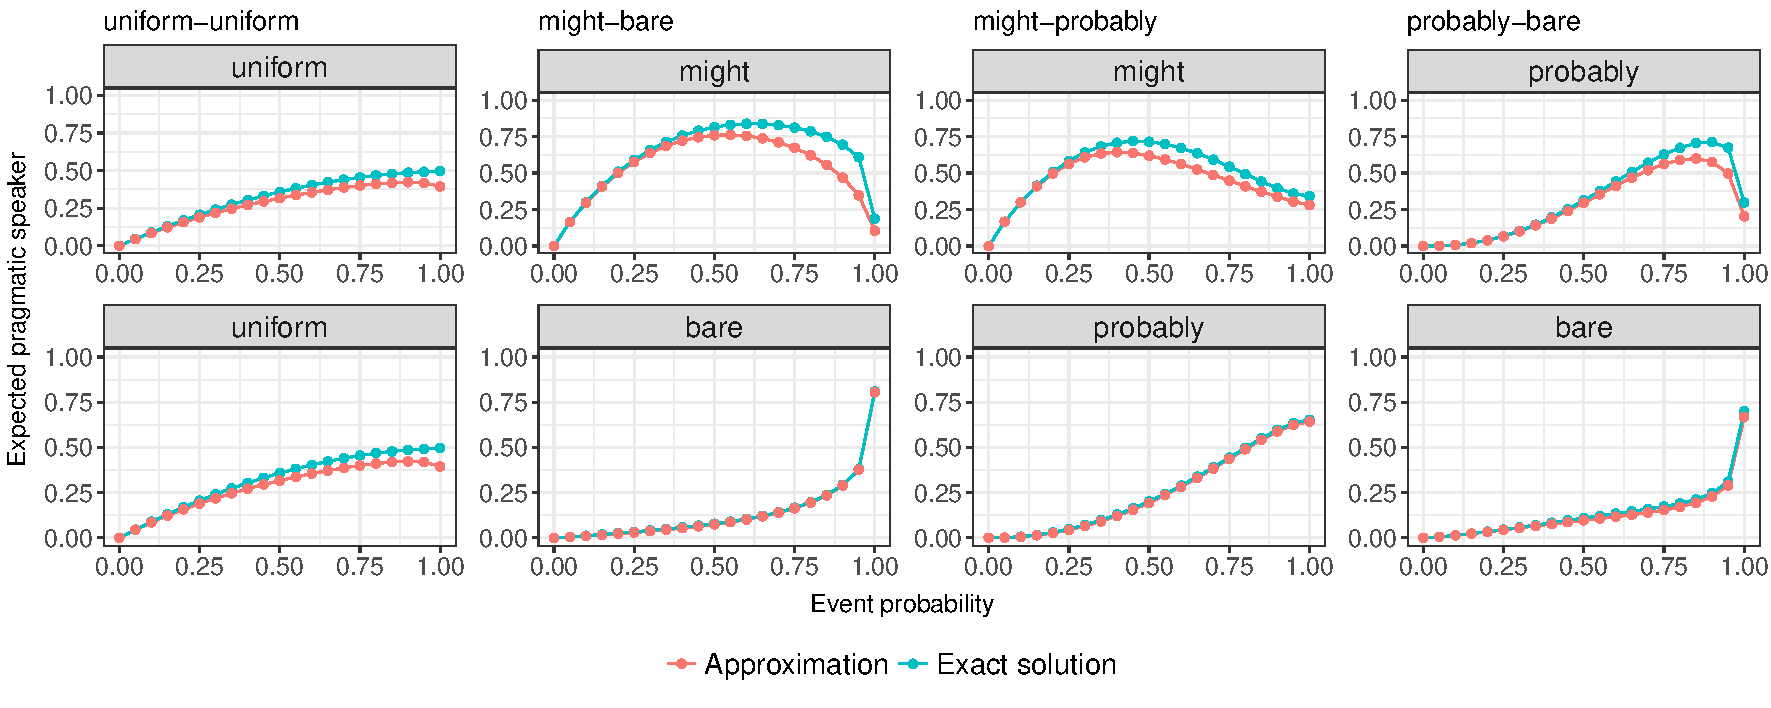
\includegraphics[width=\textwidth]{plots/approx-simulations.pdf}
\caption{Predictions of exact and approximate expected pragmatic speaker model for different combinations of thresholds. The leftmost panels (uniform) shows predictions of both models if both utterances have uniform threshold distributions, i.e., threshold distributions with very high variance. The other panels show model predictions under the assumption that the utterances have the threshold distributions that we inferred in Section~3. \label{fig:approx-simulations}}
\end{figure}

This approximation leads to identical results as $ES_1$ if each threshold distributions assigns all probability mass to one value, 
i.e., if we have point estimates for thresholds. To assess how much $ES_1$ and its approximation, $\widetilde{ES_1}$ deviate when 
the threshold distributions have non-zero variance, we performed several simulations, with different threshold distributions. For these
simulations, we assume that there are only two possible utterances, which makes the computation of $ES_1$ tractable.

Figure~\ref{fig:approx-simulations} shows the results of these simulations. As these plots show, the approximate model $\widetilde{ES_1}$ is a very close approximation of the expected
pragmatic speaker model $ES_1$, which suggests that this approximation should only minimally affect our modeling results. 

The model is implemented in Python using the scikit-learn \parencite{Scikit2011} and numpy \parencite{vanderWalt2011} libraries.

\section{Additional model predictions}
\setcounter{section}{4}


Figures~\ref{fig:norming-results-model-1} and \ref{fig:norming-results-model-2} show the model predictions and the results from all conditions in Experiment~1. 

\begin{figure}[h!]
\includegraphics[width=0.95\textwidth]{plots/pre\string_test\string_model\string_s1.pdf}
\caption{Model predictions and results of Experiment~1 -- Part 1. Error bars correspond to 95\% high density intervals (model predictions) and bootstrapped 95\%-confidence intervals (observed results). \label{fig:norming-results-model-1}}

\end{figure}

\begin{figure}[h!]
\includegraphics[width=0.95\textwidth]{plots/pre\string_test\string_model\string_s2.pdf}
\caption{Model predictions and results of Experiment~1  -- Part 2. Error bars correspond to 95\% high density intervals (model predictions) and bootstrapped 95\%-confidence intervals (observed results). \label{fig:norming-results-model-2}}

\end{figure}



\section{Original production expectation adaptation experiment}
\setcounter{section}{5}
\setcounter{subsection}{0}


We originally ran a different version of the production expectation experiment which included a potential confound because the number of utterances
with each uncertainty expression was not matched across conditions. Qualitatively, this lead to the same results as Experiment~2 in the main text 
but from this experiment, it remained unclear whether the different post-exposure ratings were a result of the different number of exposure trials
across conditions or a result of listeners updating the mapping between uncertainty expressions and event likelihoods.  

For transparency, we report the procedure and the results of the original experiment here. The procedure, materials and analyses were pre-registered at \url{https://osf.io/w926x/}.

\subsection{Method}
\subsubsection{Participants}
We recruited a total of 80 participants (40 per condition) on Amazon Mechanical Turk. 
We required participants to have a US-based IP address and a minimal approval rating 
of 95\%. Participants were paid \$2 which amounted to an hourly wage of approximately 
\$12--\$15. None of the participants had previously participated in Experiment~1.

\subsubsection{Materials and procedure}

Materials and procedure were identical to Experiment~2. The only difference between Experiment~2 and this experiment were the number of filler trials with the other uncertainty expression, as shown in Table~\ref{tbl:materials-comparison}.

\begin{table}
\centering
\begin{tabular}{l c c c c c c | c c c c c c}
\toprule
& \multicolumn{6}{c | }{Original experiment} & \multicolumn{6}{c}{Experiment 2} \\
\midrule
& \multicolumn{2}{c}{\sc might} & \multicolumn{2}{c}{\sc probably} & \multicolumn{2}{c |}{\sc bare} & \multicolumn{2}{c}{\sc might} & \multicolumn{2}{c}{\sc probably} & \multicolumn{2}{c}{\sc bare} \\
& $n$ & $\phi$ & $n$ & $\phi$ & $n$ & $\phi$ & $n$ & $\phi$ & $n$ & $\phi$ & $n$ & $\phi$\\
\midrule
\emph{cautious} & {\bf 10} & {\bf 60\%} & 5 & 90\% & 5 & 100\% & {\bf 10} & {\bf 60\%} & 10 & 90\% & 5 & 100\% \\
\emph{confident} & 5 & 25\% & {\bf 10}  & {\bf 60\%} & 5  & 100\% & 10 & 25\% & {\bf 10}  & {\bf 60\%} & 5  & 100\% \\  
\bottomrule
\end{tabular}

\caption{Number of exposure trials ($n$) per utterance ({\sc might}, {\sc probably}, {\sc bare}) 
and associated proportion of target color gumballs ($\phi$) in the \emph{cautious} vs.~\emph{confident} 
speaker conditions in this original experiment and  Experiments~2. Critical trials bolded. \label{tbl:materials-comparison}}

\end{table}

\subsubsection{Exclusions} We excluded participants who provided incorrect responses to more than 3 of the attention checks. Based on this criterion, we excluded 11 participants in the \textit{confident speaker} condition and 8 participants in the \textit{cautious speaker} condition. None of the results reported below depend on these exclusions.


\subsection{Analysis and predictions}  

As in Experiment~2, we tested whether listeners updated their expectations after exposure by computing the difference between the AUC of the spline for 
{\sc might} and of the spline for {\sc probably} for each participant. We predicted that the mean AUC difference would be larger in the 
\emph{cautious speaker} condition than in the \emph{confident speaker} condition.

\subsection{Results and discussion}

\begin{figure}
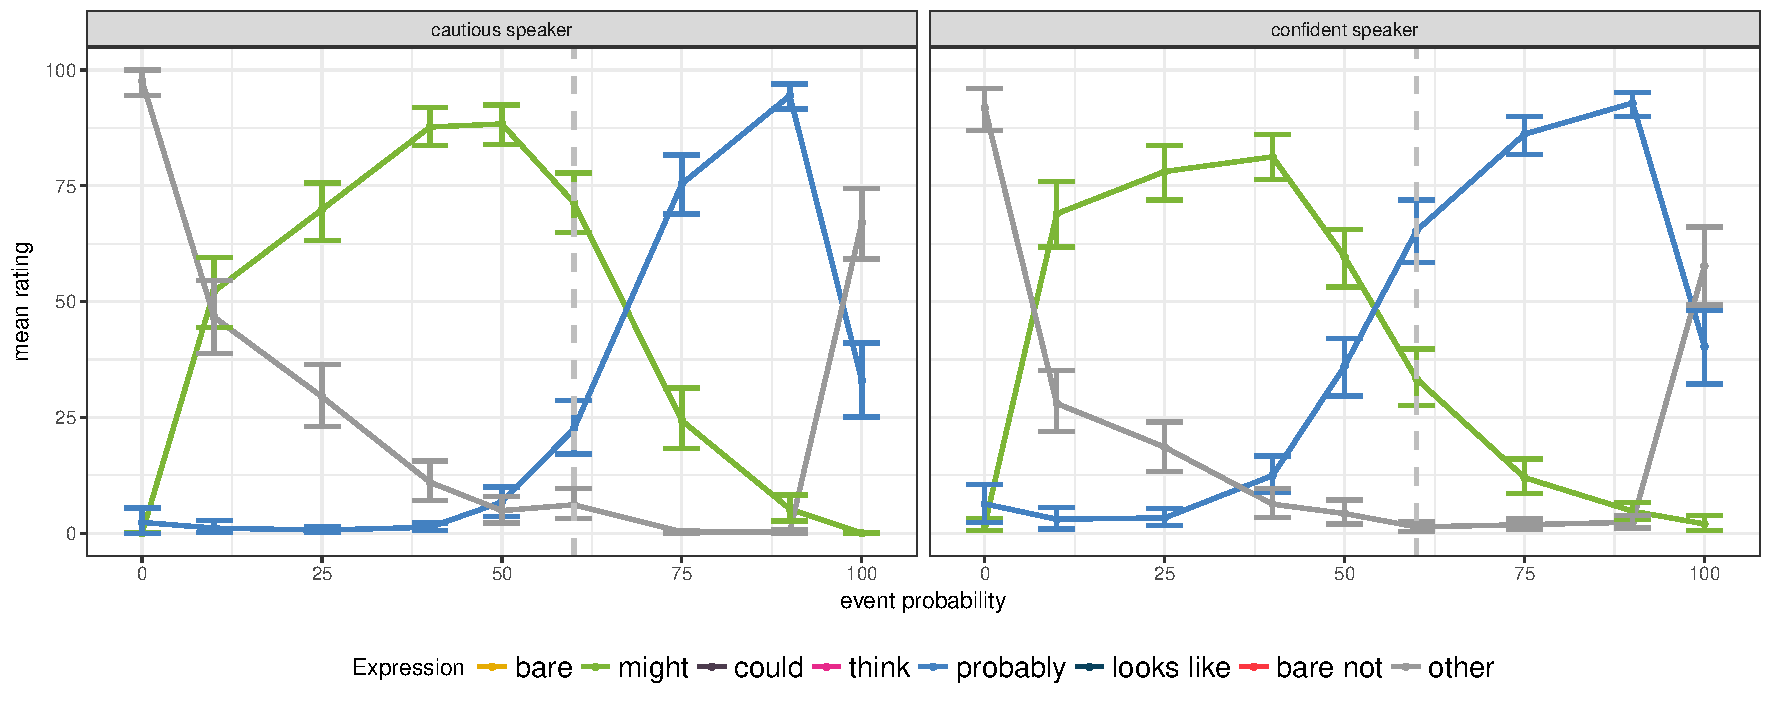
\includegraphics[width=\textwidth]{plots/exp-1-ratings.pdf}
\caption{Mean post-exposure ratings from original production expectation experiment. Error bars correspond to bootstrapped 95\%-confidence intervals.  The grey dotted line highlights the ratings for the 60\% event probability ratings.  \label{fig:adaptation-results-prod-orig}}
\end{figure}

\begin{figure}
\center
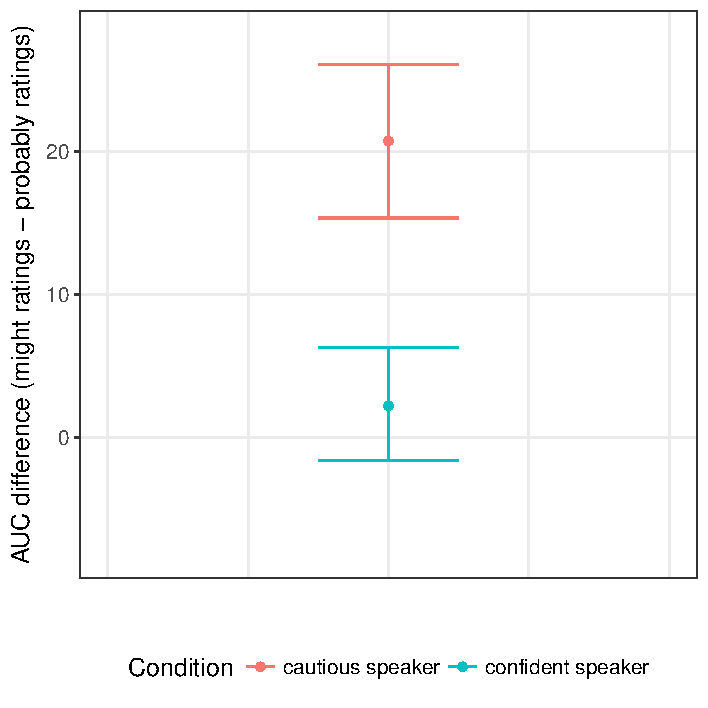
\includegraphics[width=.4\textwidth]{plots/exp-1-auc-orig.pdf}
\caption{Area under the curve (AUC) differences from original production expectation experiment. Error bars correspond to bootstrapped 95\%-confidence intervals.  \label{fig:adaptation-auc-prod-orig}}
\end{figure}

This experiment yielded the same results as Experiment~2. As the panels in Figure~\ref{fig:adaptation-results-prod-orig} show, participants updated their expectations about the speaker's language use and therefore made different predictions about how the speaker would use uncertainty expressions. In the \emph{cautious speaker} condition, participants gave high ratings for {\sc might} for a larger range of event probabilities than in the \emph{confident speaker} condition. On the other hand, participants gave high ratings for {\sc probably} for a larger range of gumball proportions in the \emph{confident speaker} condition than in the \emph{cautious speaker} condition. These differences result in a significantly larger AUC difference in the \emph{cautious speaker} condition than in the \emph{confident speaker} condition ($t(59) = 4.98$, $p < 0.001$, see also left panel of Figure~\ref{fig:adaptation-auc-prod-orig}).

However, from these results it remains unclear whether listeners update their expectations about the mapping between uncertainty expressions and event likelihoods. In this experiment, the number of utterances with \textit{might} and \textit{probably} differed across conditions. It is therefore possible that participants only learned that the {\it cautious speaker} overall prefers to use {\it might} and the {\it confident speaker} prefers {\it probably}. To address this confound, we conducted Experiment~2 which is reported in the main text.

\section{Model simulations for original production expectation experiment}
\setcounter{section}{6}


\begin{table}
\center
\begin{tabular}{r | c | c }
Model &   odds  &  $R^2$ \\ \midrule
fixed & $10^{-1137}$ &  0.746       \\
cost & $10^{-386}$ & 0.766     \\
threshold distributions & $10^{-207}$ &  0.856 \\
cost \& threshold distributions & 1 &  0.809 \\
\end{tabular}
\caption{Model evaluation results on data from original production expectation experiment.   \textit{odds} are the posterior likelihood odds of the models compared to the \textit{cost and threshold distributions} model.  $R$\textsuperscript{$2$} are computed between  the mean post-exposure ratings and the mean model predictions. \label{tbl:model-comparison-orig}}
\end{table}


Table~\ref{tbl:model-comparison-orig} shows the results of the model comparison  for the original production expectation experiment and  Figures~\ref{fig:post-exposure-model-original}, \ref{fig:post-exposure-thresholds-original}, and \ref{fig:post-exposure-costs-original} show the posterior predictions
of the model simulations, the post-adaptation threshold distributions, and the post-adaptation costs, respectively. For these simulations, we took the MAP variance parameters that we estimated for the data from Experiment~2, so we did not fit any parameters to the data from the original production expectation experiment. In each condition, the model was exposed to the 20 utterances that participants were exposed to in the experiment (see left part of Table~\ref{tbl:materials-comparison}).

These modeling results further demonstrate the stability of the results reported in the main text. We again find that the \textit{cost \& threshold distributions} model predicts the post-exposure data best according to the posterior odds metric, and the inferred post-exposure threshold distributions and cost values exhibit the same patterns as we found in the simulations for Experiment~2. Not surprisingly, the inferred cost differences between \textit{might} and \textit{probably} are bigger in the present simulations for the original experiment reflecting that the exposure across conditions was not balanced. 

However, as shown in Table~\ref{tbl:model-comparison-orig}, we also find that according to the $R^2$ metric, the model according to which listeners only update their beliefs about threshold distributions predicts the post-exposure
behavior better than the  \textit{cost \& threshold distributions} model. While we generally expect the ranking of models to be the same according to both metrics, we explained in the main text that in our setup, multiple assumptions
of the $R^2$ metric are violated and therefore, we do not consider the ranking of models according to the $R^2$ metric as evidence that listeners only update beliefs about threshold distributions -- especially given that in all other simulations, both metrics suggested that listeners update both types of representations.





\begin{figure}[h!]
  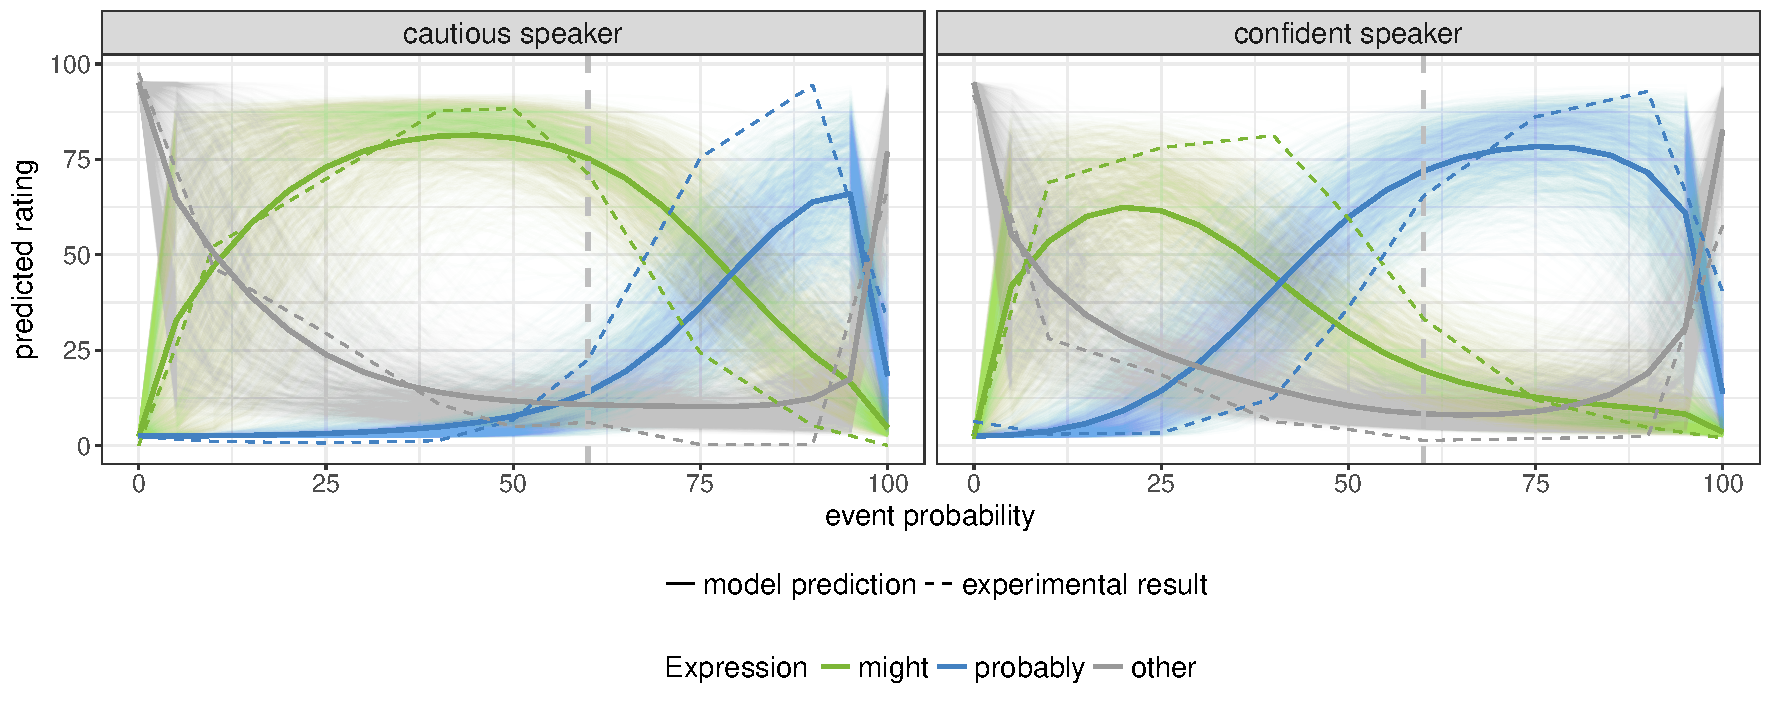
\includegraphics[width=\textwidth]{plots/adaptation-posterior-predictions.pdf}
  \caption{Post-adaptation model predictions from simulations for original production expectation experiment and experimental results. 
  The solid lines shows the mean model predictions and the thin lines around the mean show the distribution of model predictions. \label{fig:post-exposure-model-original}}
\end{figure}

\begin{figure}[h!]
  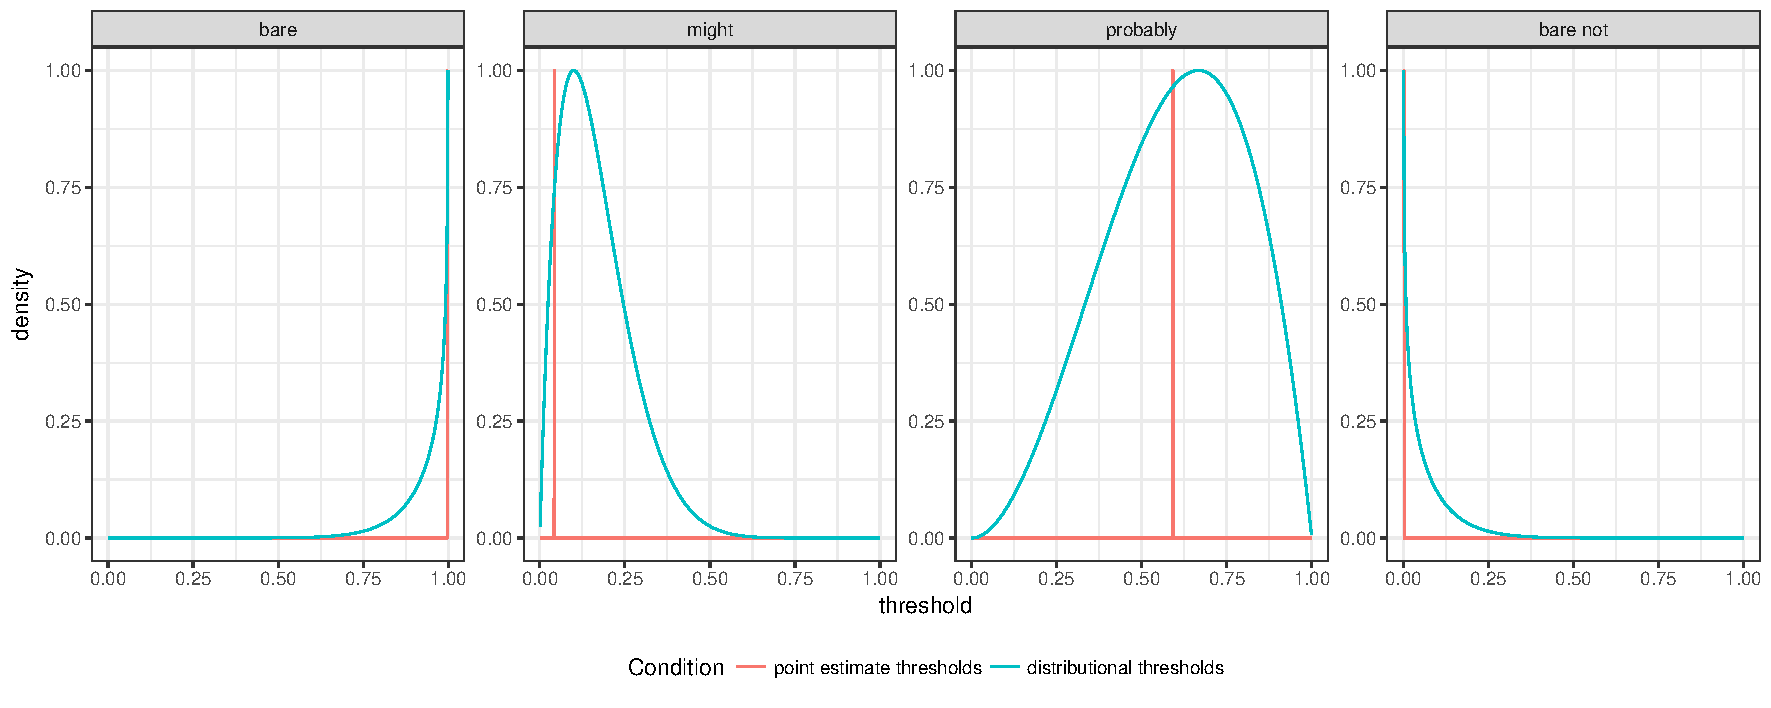
\includegraphics[width=\textwidth]{plots/adaptation-posterior-thresholds.pdf}
  \caption{Post-adaptation threshold distributions from the simulations for original production expectation experiment. \label{fig:post-exposure-thresholds-original}}
\end{figure}

\begin{figure}[h!]
\center
  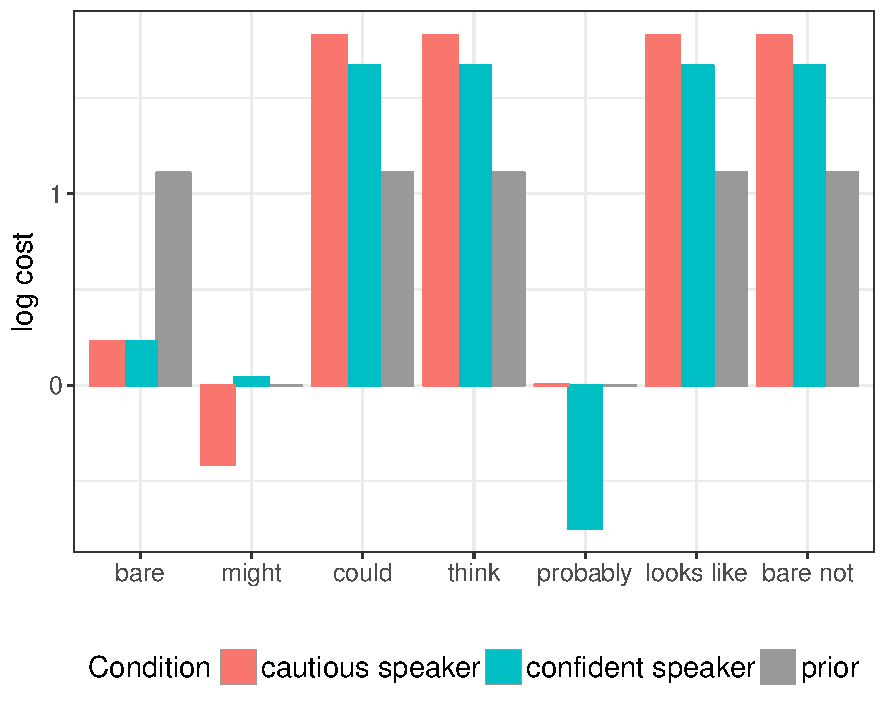
\includegraphics[width=0.5\textwidth]{plots/adaptation-posterior-costs.pdf}
  \caption{Post-adaptation $log$ cost values from simulations for for original production expectation experiment. Note that the cost of \textsc{might} and \textsc{probably} 
  in the norming data model was 1 and therefore the $log$ cost for these utterances is 0.  \label{fig:post-exposure-costs-original}}
\end{figure}

\pagebreak
\FloatBarrier



\section{Original interpretation experiment}
\setcounter{section}{7}
\setcounter{subsection}{0}

As we mentioned in the main text, we originally ran a slightly different version of the comprehension experiment in which participants used sliders to rate which gumball machine they thought the speaker was describing. While the results were qualitatively the same as in the experiment reported in the main body of the paper, the use of sliders seemed to confuse some participants (see details below) and therefore we changed the procedure such that participants provided ratings by distributing coins. For transparency, we report the 
procedure and the results of the original experiment here.

\subsection{Method}
\subsubsection{Participants}

We recruited a total of 80 participants (40 per condition) on Amazon Mechanical Turk. We required participants to have a US-based IP address and a minimal approval rating of 95\%. Participants were paid \$2 which amounted to an hourly wage of approximately \$10--\$12. None of the participants had participated in any of the previous experiments. 

\subsubsection{Materials and Procedure}

The exposure phase was identical as in the other adaptation experiments: participants were either exposed to a 
\textit{cautious} speaker or a \textit{confident} speaker. Six of the exposure trials included attention checks in which
participants had to indicate whether they saw a grey X on the previous trial or not.

Similar to Experiment~3, the test trials probed participants'
interpretations of the utterances {\sc might}, {\sc probably}, and {\sc bare}. On test trials, participants listened
to a recording of the speaker they encountered during the exposure phase and then rated how likely they
thought it was that the speaker saw different gumball machines. On each trial, like in Experiment~3, participants
provided ratings for 9 gumball machines. However, unlike in Experiment~3, participants indicated their ratings
by adjusting 9 sliders. Participants completed 6 test trials in total -- one for each expression-color pair.

\subsubsection{Exclusions}

We excluded participants who failed more than 2 out of 6 attention checks, which led to 2 exclusions in the \emph{cautious speaker} condition and 1 exclusion in the \emph{confident speaker} condition.


\subsection{Analysis and Predictions}

As for Experiment~3, we expected that listeners interpret a more confident speaker's utterance 
to communicate a lower event probability than a more cautious speaker's utterance. We measured
the interpretation of utterances by normalizing the ratings across the 9 gumball machines so that they sum to
1 and then computing the expected value for the proportion of blue and orange gumballs. 
We predicted that the expected values of target color gumball proportions after hearing {\sc might} and {\sc probably} 
were going to be larger in the \emph{cautious speaker} condition than in the \emph{confident speaker} condition.

\subsection{Results and Discussion}

\begin{figure}[h!]
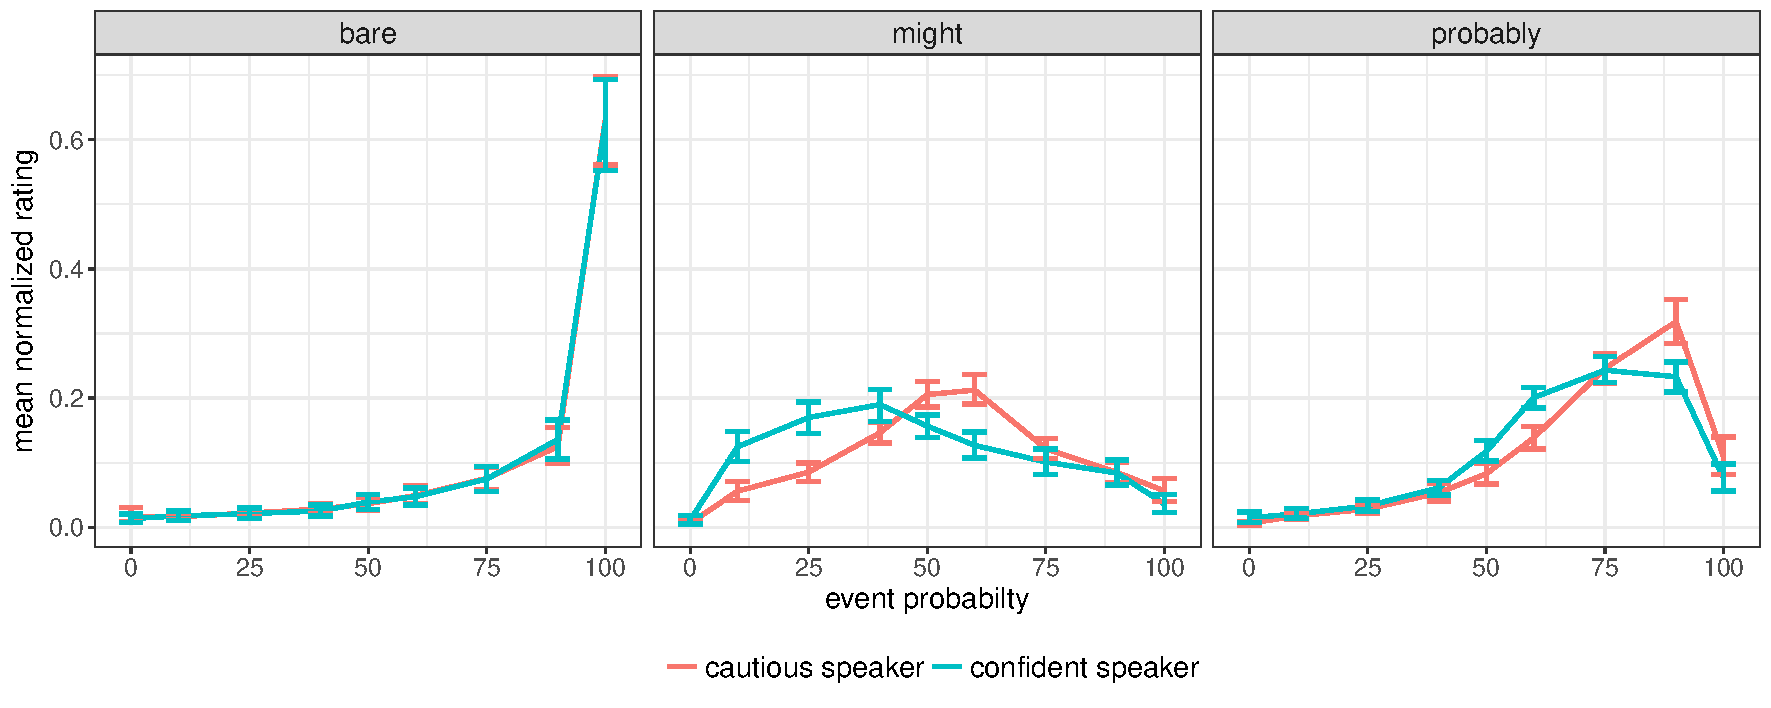
\includegraphics[width=\textwidth]{plots/exp-2-ratings-orig.pdf}
\caption{Aggregated post-exposure ratings from the original interpretation experiment.  \label{fig:adaptation-results-comp-orig}}
\end{figure}

Figure~\ref{fig:adaptation-results-comp-orig} shows the aggregated and normalized ratings for the two conditions.  As predicted, participants provided higher ratings for gumball machines with higher target color percentages after hearing {\sc might} and {\sc probably} in the \emph{cautious speaker} condition than in the \emph{cautious speaker} condition. This also led to a significantly higher expected value for {\sc might} ($t(75)=3.05$, $p<0.01$) and {\sc probably} ($t(75)=3.08$, $p<0.01$) in the \emph{cautious speaker} condition as compared to the \emph{confident speaker} condition.

This means that qualitatively, the results are the same as in Experiment~3. However, since participants had the option to assign high 
ratings to 
all gumball machines (they could assign a maximum rating to each gumball machine if they wanted to), we noticed that many participants assigned very high ratings to most gumball 
machines and therefore did not indicate their interpretation of the utterance. Further, it seemed that some participants
understood the instructions as rating the likelihood of getting a target color gumball and provided ratings proportional to the 
target color gumball proportion independent of the utterance. For these reasons, we revised the original paradigm as described
in the main text and asked participants to indicate their interpretation using a limited set of coins, which appeared to be less
confusing for participants. 



\end{document}
